% QASP software paper -- publication-oriented preprint draft.
%
% Before submission, resolve every visible \todo{...} marker and review the
% AI-use disclosure.  The manuscript deliberately does not claim a quantum
% advantage or unmeasured speedup.
%
% Suggested build:
%   latexmk -pdf main.tex
% or:
%   pdflatex main && bibtex main && pdflatex main && pdflatex main

\documentclass[10pt]{article}

\usepackage[a4paper,margin=2.25cm]{geometry}
\usepackage[T1]{fontenc}
\usepackage[utf8]{inputenc}
\usepackage{textcomp}
\usepackage{lmodern}
\usepackage{microtype}
\usepackage{amsmath,amssymb,mathtools,bm}
\usepackage{booktabs}
\usepackage{tabularx}
\usepackage{array}
\usepackage{enumitem}
\usepackage{xcolor}
\usepackage{graphicx}
\usepackage{listings}
\usepackage{caption}
\usepackage{subcaption}
\usepackage{float}
\usepackage{needspace}
\usepackage[most]{tcolorbox}
\usepackage{tikz}
\usetikzlibrary{arrows.meta,backgrounds,calc,decorations.pathreplacing,fit,positioning,shapes.geometric}
\usepackage{xurl}
\usepackage[numbers,sort&compress]{natbib}
\usepackage{hyperref}
\usepackage[capitalise,noabbrev]{cleveref}

\definecolor{qaspblue}{HTML}{2457C5}
\definecolor{qaspcyan}{HTML}{00A6A6}
\definecolor{qasppurple}{HTML}{7950C5}
\definecolor{qasporange}{HTML}{E07A2D}
\definecolor{qaspgreen}{HTML}{2E8B57}
\definecolor{qasplight}{HTML}{F3F6FC}
\definecolor{qaspfeaturebg}{HTML}{FFF3E8}
\definecolor{qaspfeaturetitle}{HTML}{8F4315}
\definecolor{codegray}{HTML}{4E5661}

\hypersetup{
  colorlinks=true,
  linkcolor=qaspblue,
  citecolor=qaspgreen,
  urlcolor=qasppurple,
  pdftitle={QASP: A Modular, differentiable and distributed software package for quantum machine learning},
  pdfauthor={Andre Sequeira}
}

\setlist[itemize]{leftmargin=*,topsep=3pt,itemsep=2pt}
\setlist[enumerate]{leftmargin=*,topsep=3pt,itemsep=2pt}
\renewcommand{\arraystretch}{1.15}

\lstdefinestyle{qasp}{
  language=Python,
  basicstyle=\ttfamily\footnotesize,
  keywordstyle=\color{qaspblue}\bfseries,
  commentstyle=\color{qaspgreen!75!black},
  stringstyle=\color{qasppurple},
  numbers=left,
  numberstyle=\tiny\color{codegray},
  numbersep=7pt,
  frame=single,
  rulecolor=\color{black!15},
  backgroundcolor=\color{qasplight},
  breaklines=true,
  breakatwhitespace=false,
  showstringspaces=false,
  keepspaces=true,
  columns=fullflexible,
  upquote=true,
  tabsize=4,
  captionpos=b
}
\lstset{style=qasp}

\newcommand{\qasp}{\textsc{Qasp}}
\newcommand{\pennylane}{\textsc{PennyLane}}
\newcommand{\torch}{\textsc{PyTorch}}
\newcommand{\todo}[1]{\textcolor{red!75!black}{\textbf{[TODO: #1]}}}
\newcommand{\code}[1]{\texttt{#1}}
\newcommand{\E}{\mathbb{E}}
\newcommand{\R}{\mathbb{R}}
\newcommand{\A}{\mathcal{A}}
\newcommand{\Hc}{\mathcal{H}}
\newcommand{\repo}{\url{https://github.com/andre-sequeira10/QASP}}
\newcommand{\version}{0.1.0}

\newtcolorbox{qaspfeature}[2][]{
  enhanced,
  colback=qaspfeaturebg,
  colframe=qasporange!78!black,
  colbacktitle=qasporange!18,
  coltitle=qaspfeaturetitle,
  fonttitle=\bfseries,
  title={QASP feature: #2},
  boxrule=0.75pt,
  arc=2.2pt,
  left=2.5mm,
  right=2.5mm,
  top=1.5mm,
  bottom=1.5mm,
  before skip=7pt,
  after skip=7pt,
  #1
}

\title{\vspace{-1.35cm}%
  
\includegraphics[width=0.70\textwidth]{figures/inesctec_logo.png}\\[0.55cm]
  \textbf{QASP: A Modular, differentiable and distributed software package for quantum machine learning}}
\author{Andr\'{e} Sequeira\\[-1mm]
  \small \todo{add affiliation, institutional address, e-mail, and ORCID}}
\date{QASP v\version{} --- September 2026}

\begin{document}
\maketitle

\begin{abstract}
We present \qasp{} (Quantum Agent Software Package), an open-source Python
framework for modular, differentiable, and distributed quantum machine
learning.  Its foundation is a set of configuration-driven building blocks for
feature maps, parameterized ansatzes, measurements, devices, gradient methods,
classical decoding, and publication-ready circuit drawings.  These primitives
support five high-level modules: reinforcement learning with configurable
quantum policies, action-value functions, and training loops; quantum kernels with fidelity,
projected-feature, alignment, and Fisher constructions; parameterized quantum
classifiers with probability or expectation readouts; generative learning with
quantum-circuit Born machines; and combinatorial optimization with QUBO
representations.  Each module
retains explicit contracts for outputs, gradients, sampling, and decoding,
enabling controlled comparisons across models and execution strategies.
High-performance experimentation is supported through optimized state-vector,
tensor-network, stabilizer, Pauli-propagation, circuit-cutting, and Kokkos/MPI
execution paths, together with analytical workload and distributed-job
planning.  QASP also provides finite-sample cost and output-concentration
diagnostics for trainability studies and exploratory utilities for sampling
policy outputs and inspecting heuristic generator closures.
Together, these layers provide a reproducible research platform spanning model
construction, task-level learning, scalable simulation, and diagnosis.
\end{abstract}

\noindent\textbf{Repository:} \repo \qquad
\textbf{License:} MIT \qquad
\textbf{Language:} Python $\geq 3.10$

\clearpage
\setcounter{tocdepth}{2}
\begingroup
\fontsize{8}{8.8}\selectfont
\tableofcontents
\endgroup
\clearpage

\section{Introduction}
\label{sec:introduction}

Variational quantum algorithms place a parameterized quantum circuit (PQC) inside a classical optimization loop.  The same pattern underlies quantum neural networks, quantum policies, and circuit Born machines: classical data are encoded into a quantum state; a trainable unitary transforms the state; measurements define a scalar, vector, or distribution-valued model output; and a classical optimizer updates the parameters.  Although the diagram is simple, a reproducible implementation must coordinate circuit topology, data re-uploading, observable design, measurement shots, differentiation, simulator capabilities, batching, and the conventions by which bit strings become labels or actions.  Small differences in any of these choices can change both the represented hypothesis class and its trainability.

The problem is especially acute in quantum reinforcement learning (QRL).  A policy must produce a valid action distribution at every environment step, and a single policy-gradient update may require many circuit evaluations.  The quantum readout may be a full Born distribution, a family of Pauli expectations, or a sampled bit string; each choice has different execution and gradient costs.  Experimental code frequently entangles these decisions with a particular environment or training loop, making controlled comparisons difficult.  At the same time, gradient concentration and barren plateaus can make apparently minor choices---observable locality, connectivity, parameter initialization, and feature scaling---scientifically decisive \cite{mcclean2018barren,larocca2022diagnosing}.

\qasp{} addresses this integration layer.  It builds on \pennylane{}'s device-independent circuit and differentiation model \cite{bergholm2018pennylane} and \torch{}'s automatic-differentiation and optimization ecosystem \cite{paszke2019pytorch}.  Rather than replacing either framework, \qasp{} contributes domain-specific abstractions for quantum agents and adjacent learning workflows.  In particular, release \version{} provides:

\begin{itemize}
  \item composable angle and neural feature maps, IQP and general Pauli-rotation ansatz templates, a measurement-aware \code{CircuitBuilder}, and configuration-resolved Matplotlib or publication-ready Quantikz circuit drawings;
  \item a vectorized decoded-Born policy core shared by probability aggregation
        and sample decoding, with contiguous, recursive-parity, hidden-parity,
        and majority--modulo action maps;
  \item exact multi-action parity reconstruction from logical Pauli moments,
        exact sparse majority action projectors, expectation-value softmax
        policies, and a learnable measurement-selection model;
  \item gradient-based training through backpropagation, adjoint differentiation,
        parameter-shift, finite differences, SPSA, and differentiable Pauli
        propagation, together with tested small-system Fisher-preconditioned
        Born-machine updates;
  \item REINFORCE, advantage-weighted contextual-bandit training, PPO
        utilities, replay-based Double DQN, Gymnasium interoperability,
        TorchRL adapters, and seeded control benchmarks;
  \item fast Pauli propagation using packed symplectic keys, plus accelerated state-vector and Kokkos execution inherited through \pennylane{} devices;
  \item one projector-configurable fidelity class for global and localized
        overlap similarities, projected expectation-feature kernels, centered
        target alignment, and a Fisher-information kernel;
  \item binary and multiclass parameterized quantum classifiers with Born or
        expectation readouts, configurable class decoders, differentiable
        losses, training utilities, and classification metrics;
  \item QUBO and Ising problem construction, standard and multi-angle QAOA,
        relaxation-based warm starts, recursive variable elimination,
        fixed linear-ramp schedules, Pauli correlation encoding, finite-shot
        solution sampling, and unified optimization results;
  \item explicit-loss quantum-circuit Born-machine training, policy-output
        variance sampling, finite-sample concentration diagnostics, and
        exploratory generator-list and Lie-closure-size utilities;
  \item workload inspection, analytical Deucalion memory/placement planning,
        Slurm-script rendering, and MPI-aware execution callbacks that keep
        resource estimates distinct from measured runtime.
\end{itemize}

This is a software paper, not an empirical claim of quantum advantage.  Its contribution is a reusable experimental substrate that makes modelling and execution choices explicit and allows like-for-like comparisons.  The presentation follows the pattern established by successful quantum-software papers: a statement of need, a concrete architecture, executable usage examples, backend boundaries, and an honest account of validation and limitations \cite{steiger2018projectq,larose2022mitiq,zhang2023tensorcircuit}.

\section{Statement of need and position in the software ecosystem}
\label{sec:need}

\subsection{Target users and research questions}

\qasp{} is aimed at researchers who need to ask questions such as:

\begin{itemize}
  \item How does a Born policy compare with an expectation-value policy under the same ansatz and optimizer?
  \item How do local, parity, hidden-qubit, or majority-based action decoders affect variance and trainability?
  \item Which conclusions survive a change from exact state-vector simulation to a tensor-network, stabilizer, distributed Kokkos, or approximate Pauli-propagation backend?
  \item Can input-scaling weights, circuit angles, observable heads, and value baselines be trained in one PyTorch computation graph?
  \item How do finite-sample output concentration and exploratory generator
        closure sizes change with connectivity, depth, and readout choice?
  \item Can the same circuit primitives be reused for a policy, a quantum
        kernel, a supervised classifier, a Born machine, and a combinatorial
        optimizer without obscuring their task-specific measurements?
  \item How do optimized, warm-started, recursive, fixed-schedule, and
        correlation-encoded QUBO solvers compare under one result and drawing
        contract?
\end{itemize}

Existing packages solve important parts of this workflow.  \pennylane{} provides a general differentiable quantum-programming layer; \torch{} supplies tensor automatic differentiation and optimizers; Gymnasium standardizes environment interaction \cite{towers2024gymnasium}; and TorchRL supplies composable data structures, collectors, actors, and losses \cite{bou2023torchrl}.  High-performance frameworks such as TensorCircuit emphasize differentiable simulation and accelerator execution \cite{zhang2023tensorcircuit}.  \qasp{} deliberately composes with these projects.  Its narrower contribution is a shared experimental layer for configurable PQC construction, research-oriented policy and classifier readouts, quantum kernels, QUBO optimization algorithms, task-level training utilities, structural diagnostics, and differentiable Pauli propagation behind consistent high-level interfaces.

\begin{table}[t]
\centering
\caption{Positioning of \qasp{} relative to the principal software layers it uses or complements.  A check mark indicates a primary, user-facing responsibility rather than every technically possible use.}
\label{tab:positioning}
\small
\begin{tabularx}{\textwidth}{@{}l*{5}{>{\centering\arraybackslash}X}@{}}
\toprule
Project & Device-agnostic circuits & Autodiff tensors & RL infrastructure & QRL policy decoders & Pauli-propagation path \\
\midrule
\pennylane{} & $\checkmark$ & via interfaces & limited & -- & specialized \\
\torch{} & -- & $\checkmark$ & foundational & -- & -- \\
Gymnasium & -- & -- & environments & -- & -- \\
TorchRL & -- & $\checkmark$ & $\checkmark$ & -- & -- \\
TensorCircuit & $\checkmark$ & $\checkmark$ & limited & -- & -- \\
\qasp{} & via \pennylane{} & via \torch{} & QRL-focused & $\checkmark$ & $\checkmark$ \\
\bottomrule
\end{tabularx}
\end{table}

\subsection{Design principles}

Five principles organize the package.

\begin{enumerate}
  \item \textbf{Separate representation from execution.}  Feature maps, ansatz templates, measurements, devices, and gradient estimators are configured independently.
  \item \textbf{Make decoder semantics explicit and invariant.}  A basis
        measurement does not become an action or class distribution until a
        documented decoder maps basis states to task labels; probability
        aggregation, expectation reconstruction, sparse projectors, and direct
        samples must realize the declared map.
  \item \textbf{Preserve end-to-end gradients.}  Trainable input scales, quantum angles, and optional classical heads remain visible to PyTorch; the differentiable Pauli engine retains the graph for surviving terms.
  \item \textbf{Fail on incompatible contracts.}  Specialized readouts validate
        shots, device, differentiation, batching, MPI, and circuit-cutting
        requirements rather than silently switching semantics.
  \item \textbf{Treat approximation as a controlled experiment.}  Pauli-weight, coefficient, and term-count thresholds are explicit parameters, not hidden defaults in the scientific result.
\end{enumerate}

\section{QASP building blocks}
\label{sec:architecture}

The package is organized around four compositional boundaries: feature maps
encode classical data, ansatz templates define trainable circuit structure,
\code{CircuitBuilder} binds measurements and execution, and high-level task
modules turn circuit outputs into learning objects.  The orange feature boxes
throughout the paper identify these public abstractions at the point where each
is introduced; the subsequent reinforcement-learning, quantum-kernel,
parameterized-classifier, generative-learning, and combinatorial-optimization
sections specialize the same building blocks to their task-level contracts.

\Cref{fig:architecture} shows the main data flow.  A user can enter through a
low-level circuit-builder interface or through the configuration-driven model,
kernel, classifier, or optimization constructors.  All routes converge on a circuit, a
measurement contract, and an execution strategy.  Task heads then interpret
the quantum result as action probabilities, classifier scores, class
probabilities, a generative distribution, a kernel feature, or a QUBO solution.

\begin{figure*}[t]
\centering
\resizebox{\textwidth}{!}{%
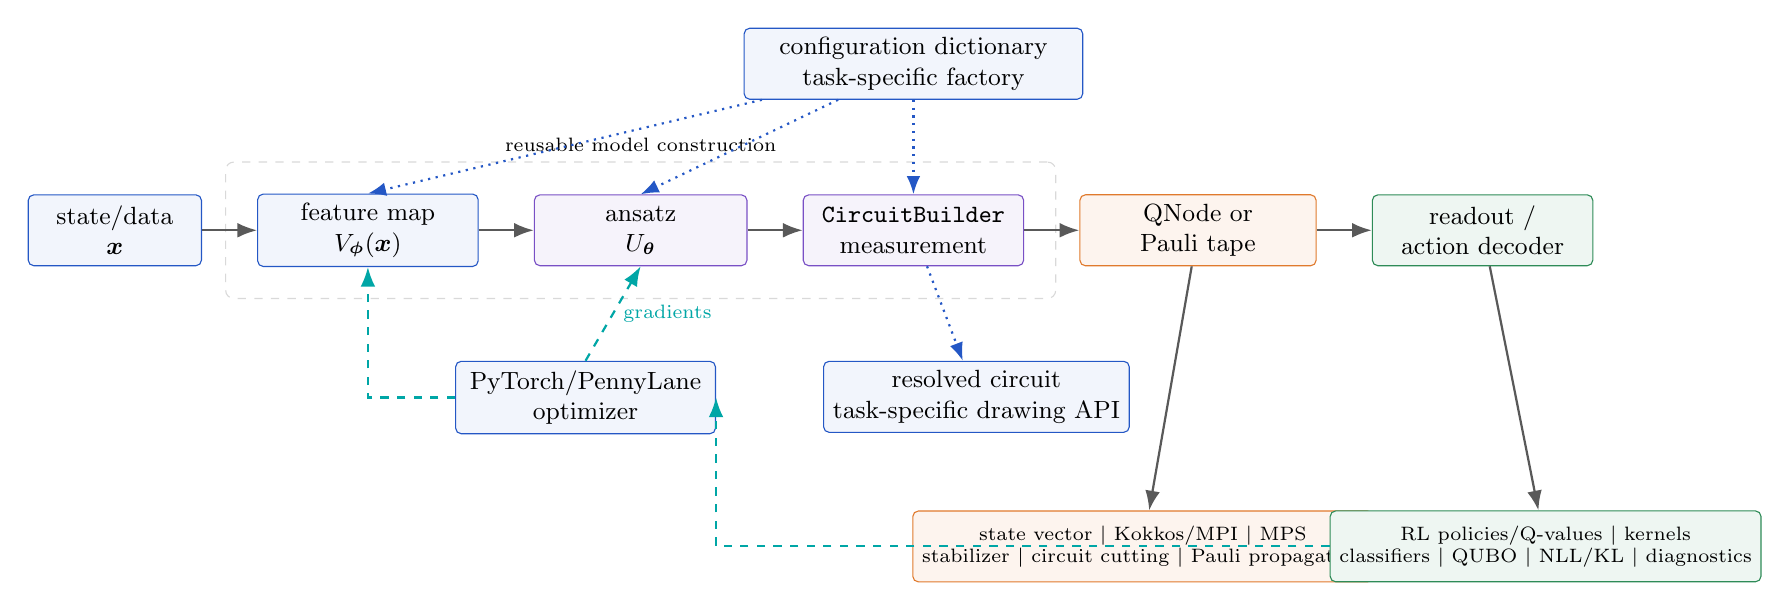
\begin{tikzpicture}[
  font=\small,
  box/.style={draw,rounded corners=2pt,minimum height=9mm,align=center,fill=white},
  data/.style={box,draw=qaspblue,fill=qaspblue!6},
  quantum/.style={box,draw=qasppurple,fill=qasppurple!7},
  exec/.style={box,draw=qasporange,fill=qasporange!8},
  task/.style={box,draw=qaspgreen,fill=qaspgreen!8},
  flow/.style={-{Latex[length=2.5mm]},thick,draw=black!65},
  grad/.style={-{Latex[length=2.5mm]},thick,dashed,draw=qaspcyan},
  inspect/.style={-{Latex[length=2.3mm]},thick,dotted,draw=qaspblue},
  node distance=8mm and 7mm
]
\node[data,minimum width=22mm] (input) {state/data\\$\bm{x}$};
\node[data,right=of input,minimum width=28mm] (fm) {feature map\\$V_{\bm{\phi}}(\bm{x})$};
\node[quantum,right=of fm,minimum width=27mm] (ansatz) {ansatz\\$U_{\bm{\theta}}$};
\node[quantum,right=of ansatz,minimum width=28mm] (builder) {\code{CircuitBuilder}\\measurement};
\node[exec,right=of builder,minimum width=30mm] (backend) {QNode or\\Pauli tape};
\node[task,right=of backend,minimum width=28mm] (readout) {readout /\\action decoder};
\node[data,above=12mm of builder,minimum width=43mm] (config) {configuration dictionary\\task-specific factory};

\draw[flow] (input) -- (fm);
\draw[flow] (fm) -- (ansatz);
\draw[flow] (ansatz) -- (builder);
\draw[flow] (builder) -- (backend);
\draw[flow] (backend) -- (readout);
\draw[inspect] (config) -- (fm.north);
\draw[inspect] (config) -- (ansatz.north);
\draw[inspect] (config) -- (builder.north);

\node[exec,below=31mm of backend,xshift=-7mm,minimum width=38mm,font=\scriptsize] (devices) {state vector $\mid$ Kokkos/MPI $\mid$ MPS\\stabilizer $\mid$ circuit cutting $\mid$ Pauli propagation};
\draw[flow] (backend) -- (devices);

\node[task,below=31mm of readout,xshift=8mm,minimum width=39mm,font=\scriptsize] (objectives) {RL policies/Q-values $\mid$ kernels\\classifiers $\mid$ QUBO $\mid$ NLL/KL $\mid$ diagnostics};
\draw[flow] (readout) -- (objectives);

\node[data,below=12mm of ansatz,xshift=-7mm,minimum width=33mm] (optim) {PyTorch/PennyLane\\optimizer};
\node[data,below=12mm of builder,xshift=8mm,minimum width=36mm] (drawing) {resolved circuit\\task-specific drawing API};
\draw[inspect] (builder) -- (drawing);
\draw[grad] (objectives.west) -| (optim.east);
\draw[grad] (optim.north) -- node[right,font=\scriptsize,text=qaspcyan]{gradients} (ansatz.south);
\draw[grad] (optim.west) -| (fm.south);

\begin{scope}[on background layer]
  \node[draw=black!15,dashed,rounded corners=3pt,fit=(fm)(ansatz)(builder),inner sep=4mm,label={[font=\scriptsize]above:reusable model construction}] {};
\end{scope}
\end{tikzpicture}
}
\caption{High-level \qasp{} architecture.  Solid arrows denote the forward
path, dashed cyan arrows differentiable feedback, and dotted blue arrows
configuration or inspection.  Task-specific factories resolve the same
components exposed by the low-level builder, while \code{draw\_model},
\code{draw\_qfunction},
\code{draw\_kernel}, \code{draw\_classifier}, and
\code{draw\_optimization} visualize their executable circuits.  One
construction can feed different task heads and backends.}
\label{fig:architecture}
\end{figure*}

\begin{qaspfeature}{\code{create\_model} and \code{draw\_model}}
\code{create\_model(policy\_class, config, n\_qubits)} is the high-level model
factory.  It resolves string-valued feature maps, ansatz templates, policy
classes, measurements, devices, and differentiation methods into one PyTorch
module.  \code{draw\_model} accepts that resolved module and renders the circuit
that will actually execute.  Its \code{output} option selects an interactive
Matplotlib drawing or editable, vector-quality Quantikz source, making the
configuration dictionary both a model specification and an inspectable
experiment record.
\end{qaspfeature}

\begin{table}[p]
\centering
\caption{Module map for release \version{}.  ``Experimental'' denotes a research-facing API that may evolve; it does not imply that the module is unused.}
\label{tab:modules}
\scriptsize
\renewcommand{\arraystretch}{1.06}
\begin{tabularx}{\textwidth}{@{}p{0.28\textwidth}X>{\raggedright\arraybackslash}p{0.12\textwidth}@{}}
\toprule
Module & Responsibility & Status \\
\midrule
\code{qasp.circuits.constructor} & Circuit assembly; probability, state, sample, expectation, and variance measurements; device and gradient selection; adaptive measurements; TorchLayer creation. & Core \\
\code{qasp.circuits.templates} & \code{IQPAnsatz} and \code{AngleAnsatz}; topology, rotations, entanglers, re-uploading, and parameter-shape calculation. & Core \\
\code{qasp.circuits.tikz} & Quantikz export from builders, QNodes, quantum functions, or tapes; symbolic labels, semantic gate colors, wire labels, standalone documents, and repeated-layer compression. & Core \\
\code{qasp.circuits.uqc} & Retained historical UQC function with an older broadcast interface and unresolved imports; not a supported template path. & Legacy \\
\code{qasp.feature\_maps.templates} & \code{AngleEmbedding} and \code{NeuralEmbedding}, with optional input scaling and entangling patterns. & Core \\
\code{qasp.devices} & Shared PennyLane device creation with explicit backend and MPI option propagation; no silent serial fallback. & Core \\
\code{qasp.rl.model} & Configuration resolution, \code{create\_model}, and circuit visualization through \code{draw\_model}. & Core \\
\code{qasp.rl.policies} & Born, enhanced Born/variance, softmax, and adaptive-measurement models; one vectorized decoder for probability and sample paths; logical-moment reconstruction; exact sparse projectors. & Core \\
\code{qasp.rl.qfunctions} & Differentiable \code{PQDQN} action-value models; shared and per-action features, parity and majority support presets, configurable affine bias and preset size, QNode or QASP Pauli execution, and configuration/drawing factories. & Research \\
\code{qasp.rl.pp\_sim} & Packed-key, non-differentiable fast truncated Pauli propagation. & Experimental \\
\code{qasp.rl.}\linebreak\code{differentiable\_pp\_sim} & PyTorch-connected Pauli propagation with differentiable retained coefficients. & Experimental \\
\code{qasp.rl.torchrl} & Episode-batched REINFORCE, replay-based Double DQN, contextual-bandit AWR, PPO utilities, value baselines, Gymnasium environment, and TorchRL adapter. & Research \\
\code{qasp.rl.trl} & Historical TorchRL PPO prototype retained for compatibility; the maintained trainer implementations live in \code{qasp.rl.torchrl}. & Legacy \\
\code{qasp.rl.envs} & Seed-reproducible \code{WindyTargetNavigationEnv} with three or four thrust actions, persistent wind, inertial dynamics, and waypoint rewards. & Research \\
\code{qasp.rl.metrics} & Policy-output variance sampling and optional Ray parallelism, plus legacy exploratory routines that return heuristic generator lists or Lie-closure sizes rather than certified circuit algebras. & Experimental \\
\code{qasp.diagnostics.}\linebreak\code{barren\_plateau} & Model-agnostic finite-sample cost concentration for classifiers, trainable kernels, and RL policies. & Research \\
\code{qasp.qkernels.}\linebreak\code{quantum\_kernels} & One projector-configurable \code{FidelityKernel} for global and localized overlap similarities, projected expectation-feature kernels, trainable ansatz support, and differentiable Gram matrices. & Core \\
\code{qasp.qkernels.factory} & Configuration-driven \code{create\_kernel} and \code{draw\_kernel} entry points. & Core \\
\code{qasp.qkernels.kta} & Centered kernel--target alignment and gradient-based kernel fitting. & Research \\
\code{qasp.qkernels.kernels} & Small-system Fisher-score Gram matrices for bit-string data; exhaustive basis enumeration, zero-probability sensitivity, and an unused legacy normalization option. & Experimental \\
\code{qasp.classifiers.models} & Binary and multiclass \code{PQCClassifier} models with probability or expectation readouts. & Core \\
\code{qasp.classifiers.decoders} & Contiguous, recursive-parity, and majority--modulo class-probability aggregation and sample decoding. & Core \\
\code{qasp.classifiers.}\linebreak\code{losses, training} & Differentiable supervised objectives and minibatch PyTorch training. & Core \\
\code{qasp.classifiers.metrics} & Confusion-matrix, accuracy, F1, calibration, ROC-AUC, and PR-AUC evaluation. & Core \\
\code{qasp.genlearn.models} & \code{PQCBM} construction and training with Torch or Autograd, probability NLL or expectation-mixture MMD, optional fixed conditioning features, direct device sampling, and a deprecated \code{BornMachine} compatibility wrapper. & Research \\
\code{qasp.genlearn.losses} & Negative log likelihood, Kullback--Leibler helpers, Gaussian MMD$^2$, binary-index conversion, exact or sampled Pauli-mask mixtures, and finite-shot corrections. & Research \\
\code{qasp.genlearn.}\linebreak\code{factory, drawing} & Configuration-driven \code{create\_qcbm} and text, Matplotlib, or publication-ready Quantikz circuit export. & Core \\
\code{qasp.optimization.problem} & QUBO construction, exact energy evaluation, QUBO--Ising conversion, Hamiltonians, and brute-force references. & Core \\
\code{qasp.optimization.qaoa} & Standard, multi-angle, warm-start, and fixed linear-ramp QAOA with analytic or finite-shot execution. & Research \\
\code{qasp.optimization.recursive} & Correlation-driven recursive QAOA reduction, exact cutoff solution, and assignment reconstruction. & Research \\
\code{qasp.optimization.pce} & Pauli correlation encoding with dictionary-defined QASP ansatz circuits and soft-spin decoding. & Research \\
\code{qasp.optimization.}\linebreak\code{optimizers, drawing, results} & SciPy optimizer adapters, common result containers, and text, Matplotlib, or Quantikz circuit drawings. & Core \\
\code{qasp.hpc.workload, planner} & Side-effect-free workload inspection and conservative Deucalion memory/placement estimates from a dated hardware profile. & Research \\
\code{qasp.hpc.slurm, run} & Slurm-script rendering and MPI-aware execution callbacks; scripts are generated but never submitted or used to transfer/install code. & Research \\
\bottomrule
\end{tabularx}
\end{table}

\subsection{Composable quantum models}
\label{sec:models}

Let $n$ be the number of model qubits, $\bm{x}\in\R^d$ an input, $\bm{\phi}$ trainable encoding parameters, and $\bm{\theta}$ variational circuit parameters.  The common \qasp{} model state is
\begin{equation}
  \lvert\psi_{\bm{\theta},\bm{\phi}}(\bm{x})\rangle
  = U_{\bm{\theta},\bm{\phi}}(\bm{x})\lvert 0\rangle^{\otimes n},
  \qquad
  U_{\bm{\theta},\bm{\phi}}(\bm{x})
  = \prod_{\ell=1}^{L} W_{\bm{\theta}_{\ell}}V_{\bm{\phi}_{\ell}}(\bm{x}),
  \label{eq:model}
\end{equation}
where the order and presence of the first or repeated $V$ blocks are configurable.  This factorization is deliberately schematic: a template may place encoders before selected layers, omit final entanglers, or use explicit Pauli words rather than a uniform gate family.

\subsubsection{Feature maps}

\code{AngleEmbedding} supports two input modes.  If \code{rotations} is a string such as \code{"YZ"}, each character selects a PennyLane angle-embedding rotation over the model wires.  If it is a list such as \code{"ZZ 0 1"}, entry $x_j$ controls the corresponding Pauli rotation
\begin{equation}
  R_{P_j}(x_j)=\exp\!\left(-\frac{i}{2}x_jP_j\right),
  \qquad P_j\in\{I,X,Y,Z\}^{\otimes n}.
\end{equation}
With input scaling, $x_j$ is replaced by $\phi_jx_j$.  Optional CNOT or CZ patterns can be specified as a chain, ring, all-to-all graph, explicit edge list, or callable topology.

\begin{qaspfeature}{\code{AngleEmbedding}}
A direct data encoder for angle and Pauli rotations.  It maps input coordinates
to configured generators, optionally learns multiplicative input scales, and
supports reusable entangling patterns.  Use it when input coordinates already
have a meaningful one-to-one relationship with circuit rotations.
\end{qaspfeature}

\code{NeuralEmbedding} assigns a trainable bias-free linear projection to each
rotation site.  For wire or Pauli word $j$ it applies
\begin{equation}
  R_{P_j}\!\left(\langle\bm{\phi}_j,\bm{x}\rangle\right).
  \label{eq:neural_embedding}
\end{equation}
Thus a small observation vector can drive many circuit locations without a
separate classical network.  Both $\bm{\phi}$ and $\bm{\theta}$ are registered
in the resulting \code{qml.qnn.TorchLayer} and can be assigned different
optimizer groups.  The current reduction is single-sample; batched workloads
should evaluate samples sequentially rather than assume broadcast support.

\begin{qaspfeature}{\code{NeuralEmbedding}}
A trainable linear quantum embedding.  Every configured rotation receives a
learned projection of the complete classical input, allowing a low-dimensional
state to drive many circuit sites while preserving gradients to the projection
weights.  It is the default embedding in the CartPole and windy-navigation
examples.
\end{qaspfeature}

\subsubsection{Ansatz families}

\code{AngleAnsatz} is the general template.  Each layer contains an arbitrary sequence of single- or multi-qubit Pauli rotations, followed optionally by fixed CNOT or CZ entanglers.  Rotation strings such as \code{"ZY"} broadcast one-qubit rotations over all wires; lists such as \code{["Y 0", "ZZ 0 1"]} define an explicit generator set.  The template exposes data re-uploading \cite{perezsalinas2020data}, custom topology, optional initial Hadamards, and control over initial and final feature-map or entangler blocks.

\begin{qaspfeature}{\code{AngleAnsatz}}
The general layered ansatz abstraction.  Users select local or multi-qubit
Pauli generators, layer count, feature-map placement, re-uploading, entangler
type, and graph topology.  Its explicit parameter-shape contract is consumed
by \code{CircuitBuilder} when constructing a differentiable Torch layer.
\end{qaspfeature}

\code{IQPAnsatz} constructs commuting phase-and-entangler blocks inspired by instantaneous quantum polynomial circuits.  For one layer with local terms and edge set $E$, its implemented form is
\begin{equation}
  H^{\otimes n}
  \left(\prod_{j=1}^{n}R_{Z_j}(\theta_j)\right)
  \left(\prod_{(j,k)\in E}R_{Z_jZ_k}(\theta_{jk})\right)
  H^{\otimes n},
  \label{eq:iqp}
\end{equation}
with repeated blocks, optional local rotations, and optional feature-map insertion.  The explicit parameter-shape methods on both ansatz classes prevent a common class of silent indexing errors when constructing Torch layers.

\begin{qaspfeature}{\code{IQPAnsatz}}
A graph-configurable IQP template built from commuting local and edge phase
generators.  It supports repeated layers, optional local terms, feature-map
insertion, and string or explicit-edge topologies.  The same abstraction feeds
trainability analysis, exact simulators, Pauli propagation, and the matched RL
experiments.
\end{qaspfeature}

\code{UQC} records an earlier functional experiment with affine data angles.
It retains unresolved imports and an obsolete broadcast convention, so it is
documented for provenance rather than presented as an executable release
template.  New models should implement the class-based ansatz contract.

\begin{qaspfeature}{Legacy \code{UQC}}
A historical functional circuit kept to make older experiments interpretable.
Its current source is not a supported construction path; \code{AngleAnsatz}
and \code{IQPAnsatz} are the maintained extension points.
\end{qaspfeature}

\begin{figure}[t]
\centering
\resizebox{\textwidth}{!}{%
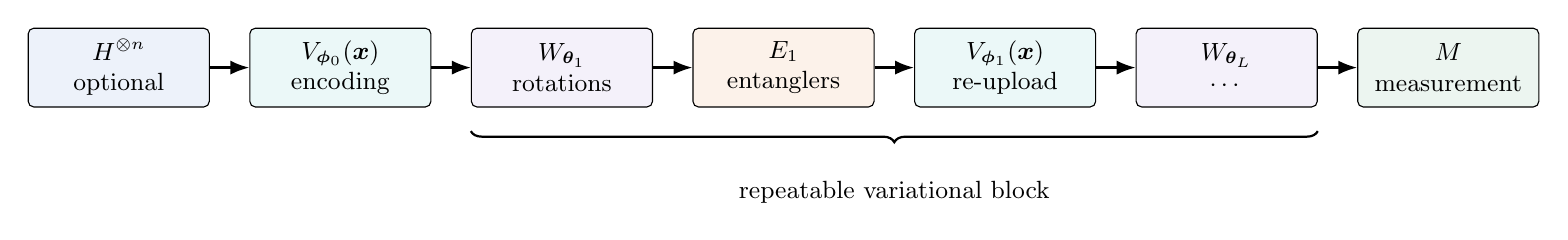
\begin{tikzpicture}[
  font=\small,
  block/.style={draw,rounded corners=2pt,minimum width=23mm,minimum height=10mm,align=center},
  arrow/.style={-{Latex[length=2.4mm]},thick},
  node distance=5mm
]
\node[block,fill=qaspblue!8] (h) {$H^{\otimes n}$\\optional};
\node[block,fill=qaspcyan!8,right=of h] (v0) {$V_{\bm{\phi}_0}(\bm{x})$\\encoding};
\node[block,fill=qasppurple!8,right=of v0] (w1) {$W_{\bm{\theta}_1}$\\rotations};
\node[block,fill=qasporange!10,right=of w1] (e1) {$E_1$\\entanglers};
\node[block,fill=qaspcyan!8,right=of e1] (v1) {$V_{\bm{\phi}_1}(\bm{x})$\\re-upload};
\node[block,fill=qasppurple!8,right=of v1] (wl) {$W_{\bm{\theta}_L}$\\$\cdots$};
\node[block,fill=qaspgreen!9,right=of wl] (m) {$M$\\measurement};
\foreach \a/\b in {h/v0,v0/w1,w1/e1,e1/v1,v1/wl,wl/m}{\draw[arrow] (\a)--(\b);}
\draw[decorate,decoration={brace,amplitude=4pt,mirror},thick]
  ($(w1.south west)+(0,-3mm)$) -- ($(wl.south east)+(0,-3mm)$)
  node[midway,below=5mm]{repeatable variational block};
\end{tikzpicture}
}
\caption{A configurable \qasp{} circuit.  The initial Hadamards, feature-map placement, re-uploading, generator sequence, topology, and final entangler are independently selectable.}
\label{fig:circuit}
\end{figure}

\subsubsection{CircuitBuilder and measurement contracts}

\code{CircuitBuilder} separates circuit definition from execution.
\code{build()} returns a plain quantum function; after the ansatz and
measurement are fixed, \code{compile()} creates the device-bound QNode, and
\code{create\_torchlayer()} allocates its trainable weights.  Merely calling
\code{set\_feature\_map()} stores metadata: the encoding must also be attached
to the ansatz that queues the gates.  The measurement contract supports full
or marginal probabilities, state vectors, samples, expectation values, and the
explicit name \code{"variance"}.  Observable strings such as
\code{"ZZ 0 1"} are parsed into Pauli words; constructed PennyLane operators
are accepted directly, enabling sparse action projectors.

The adaptive builder variant accepts both data and a run-time measurement specification.  It is used by \code{LearnablePQCBorn} to select a measurement subset from the observation.  Keeping this logic in the builder ensures that policies and non-RL models use the same circuit conventions.

\begin{qaspfeature}{\code{CircuitBuilder}}
The low-level assembly and execution boundary.  It combines an ansatz with a
measurement contract, returns a plain quantum function from \code{build()},
binds a backend and differentiation method in \code{compile()}, and then can
allocate a \code{qml.qnn.TorchLayer}.
Probability, state, sample, expectation, variance, adaptive-measurement, and
sparse-observable outputs share this interface.
\end{qaspfeature}

\begin{qaspfeature}{\code{circuit\_to\_tikz}, \code{save\_tikz}, and paper-ready drawings}
Any \code{CircuitBuilder}, PennyLane QNode, quantum function, or recorded tape
can be exported as editable Quantikz source.  The same path is exposed by
\code{CircuitBuilder.to\_tikz}, \code{draw\_model(output="tikz")}, and
\code{draw\_kernel(output="tikz")}.  Users may request symbolic parameters,
custom wire labels and semantic gate colors, a complete standalone document,
or compressed repeated layers in which the first layer remains explicit and
later layers become register-wide $U(\bm\theta_\ell)$ blocks.  The output is
vector LaTeX, so circuit typography and line weights follow the paper rather
than a raster screenshot.  Measurement meters represent quantum readouts; any
classical affine head, decoder, or reconstruction coefficients remain external
and must be stated in the caption or accompanying equations.
\end{qaspfeature}

The legacy initializer name \code{discrete\_0\_pi\_over\_2} should not be read
as a mathematical contract: the present builder samples the two values $0$ and
$\pi$.  Throughout this paper we therefore report the actual initialization
values or use an unambiguous initializer name.

\begin{lstlisting}[caption={Low-level construction of a differentiable quantum layer.  The snippet uses public release-\version{} interfaces.},label={lst:builder}]
import pennylane as qml
import torch
from qasp import AngleEmbedding, AngleAnsatz, CircuitBuilder

feature_map = AngleEmbedding(
    n_qubits=4, features=4, rotations="YZ", input_scaling=True
)
ansatz = AngleAnsatz(
    n_qubits=4,
    n_layers=3,
    rotations="ZY",
    feature_map=feature_map,
    reuploading=True,
    include_imprimitive=True,
    imprimitive="CZ",
    imprimitive_pattern="ring",
)

builder = CircuitBuilder(n_qubits=4)
builder.set_ansatz(ansatz)
builder.set_measurement(
    "expectation",
    wires=range(4),
    observables=["Z 0", "Z 1", "ZZ 0 1", "ZZ 2 3"],
)
builder.build()
builder.compile(device="lightning.qubit", diff_method="adjoint")
quantum_layer = builder.create_torchlayer(initialization="small_normal")

x = torch.tensor([0.1, -0.2, 0.3, 0.5])
loss = quantum_layer(x).square().mean()
loss.backward()  # gradients for circuit and input-scaling parameters
\end{lstlisting}

\subsection{Gradient-based optimization}
\label{sec:gradients}

Gradient flow is a cross-cutting concern in \qasp{}, not a trainer-specific
feature.  The package supports three distinct but interoperable layers:
PennyLane differentiates device-bound QNodes;
\code{qml.qnn.TorchLayer} registers the resulting parameters with PyTorch; and
task-level code differentiates RL, kernel, classifier, or generative
objectives.  The optimization module uses the same PennyLane derivative layer
for QAOA Hamiltonian expectations and hands values or Jacobians to a reusable
SciPy optimizer adapter.

\subsubsection{Device-mediated derivatives}

The \code{diff\_method} argument is forwarded to PennyLane.  Depending on device and measurement support, users can select backpropagation, adjoint differentiation, parameter-shift, finite differences, SPSA, or PennyLane's \code{"best"} dispatch.  For a gate generated by a two-eigenvalue Pauli operator, the familiar parameter-shift identity is
\begin{equation}
  \frac{\partial f}{\partial\theta_j}
  = \frac{1}{2}\left[f\!\left(\theta_j+\frac{\pi}{2}\right)
  -f\!\left(\theta_j-\frac{\pi}{2}\right)\right],
  \label{eq:paramshift}
\end{equation}
which permits hardware-compatible analytic gradients \cite{schuld2019gradients}.  Adjoint differentiation instead propagates derivative information through an analytic simulator and is particularly effective when many parameters feed a small number of expectation values.  SPSA uses simultaneous random directions and can reduce circuit-query dependence on parameter count at the cost of stochastic derivative noise \cite{spall1992spsa}.

These methods are not interchangeable for every measurement.  \qasp{} therefore keeps the requested measurement and derivative method visible and adds validation for specialized combinations such as sparse-projector adjoints.  \Cref{tab:gradients} summarizes the intended usage; the installed PennyLane device remains the final authority on a particular combination.

\begin{qaspfeature}{Differentiable QNodes and Torch layers}
\code{CircuitBuilder.compile} binds the selected PennyLane device and
derivative method, while \code{create\_torchlayer} registers circuit and
embedding parameters with PyTorch.  Backpropagation, adjoint,
parameter-shift, finite-difference, and SPSA estimators therefore meet the same
task-level optimizer interface, subject to device and measurement support.
\end{qaspfeature}

For QAOA, \code{diff\_method="auto"} selects adjoint differentiation under
analytic execution and parameter shift when the training device has finite
shots.  A derivative-aware optimizer such as BFGS receives
\code{QAOA.gradient} when \code{use\_gradients=True}; derivative-free methods
such as COBYLA instead minimize the same analytic or noisy Hamiltonian
expectation directly.  The shot count used to report the final bit-string
distribution is configured independently from the training shot count.

\begin{table}[t]
\centering
\caption{Gradient and optimization paths exposed by \qasp{}.  ``Analytic'' refers to shots set to \code{None}; finite-shot compatibility depends on the selected PennyLane device and estimator.}
\label{tab:gradients}
\small
\begin{tabularx}{\textwidth}{@{}p{0.19\textwidth}p{0.19\textwidth}X p{0.20\textwidth}@{}}
\toprule
Path & Typical outputs & Strength & Principal boundary \\
\midrule
Backpropagation & probabilities or expectations & Native autodiff through simulator & Simulator-only; memory can scale as a state vector \\
Adjoint & expectations & Many-parameter gradients without two shifts per parameter & Analytic expectation-oriented devices \\
Parameter-shift & probabilities or expectations & Analytic, hardware-compatible rule & Circuit evaluations generally grow with differentiated gates \\
Finite difference & general scalar/vector outputs & Broad fallback and gradient checking & Step-size bias and cancellation \\
SPSA & stochastic objectives & Query-efficient directions in high dimension & Higher estimator variance \\
Natural gradient & Born-machine loss & Geometry-aware preconditioning with quantum/classical Fisher matrix & Fisher construction and linear solve \\
Differentiable PP & Pauli expectations & Backpropagation through retained operator paths & Approximation and supported-gate restrictions \\
\bottomrule
\end{tabularx}
\end{table}

\subsubsection{Readout-aware gradient equivalence}

Let $\bm r_{\bm\Theta}(s)$ denote the raw circuit output and
$g$ the differentiable readout map, so that
$\bm\pi_{\bm\Theta}(s)=g(\bm r_{\bm\Theta}(s))$.  For a scalar learning
objective $\mathcal L$, the hybrid chain rule is
\begin{equation}
  \nabla_{\bm\Theta}\mathcal L
  =J_{\bm r}(\bm\Theta)^{\mathsf T}
   J_g(\bm r)^{\mathsf T}
   \nabla_{\bm\pi}\mathcal L.
  \label{eq:readout-chain-rule}
\end{equation}
The readout Jacobian is explicit in every QASP path.  For the full-probability
route, $g(\bm p)=D\bm p$ and $J_g=D$.  For the moment route,
\cref{eq:fwht} gives
\begin{equation}
  \frac{\partial p(z)}{\partial\theta_j}
  =2^{-m}\sum_t(-1)^{t\cdot z}
    \frac{\partial\mu_t}{\partial\theta_j},
  \label{eq:moment-gradient}
\end{equation}
so the FWHT commutes with differentiation.  For a sparse action projector,
linearity gives the exact identity
\begin{equation}
  \frac{\partial}{\partial\theta_j}\langle\Pi_a\rangle
  =\sum_{z:\,d(z)=a}
    \frac{\partial p(z)}{\partial\theta_j}.
  \label{eq:projector-gradient-equivalence}
\end{equation}
Accordingly, full probabilities, logical moments, and sparse projectors must
produce the same gradients whenever they implement the same $d$ and use exact
analytic execution.  QASP treats this equality as a regression invariant, not
as a backend assumption.  The only extra operation in the sparse output path
is roundoff protection at the probability-simplex boundary.

\subsubsection{Hybrid parameter groups}

A constructed Torch layer may contain circuit parameters $\bm{\theta}$ and input-scaling parameters $\bm{\phi}$.  Softmax policies can add a classical readout $(W,\bm{b})$ and a scale $\beta$; RL trainers may add a value network.  \qasp{} exposes these as ordinary PyTorch trainables, so a user can select separate learning rates,
\begin{equation}
  \bm{\Theta}\leftarrow
  \bm{\Theta}-\eta\,\widehat{\nabla_{\bm{\Theta}}\mathcal{L}},
  \qquad
  \bm{\Theta}=\{\bm{\theta},\bm{\phi},W,\bm{b},\beta\}.
\end{equation}
The training utilities explicitly collect nonstandard leaf tensors from a PennyLane Torch layer when needed.  The TorchRL-oriented trainer additionally verifies that a nonzero finite gradient reaches at least one trainable, and the RL optimizers optionally clip the global gradient norm.

\subsubsection{Small-system natural-gradient branch}

The \code{PQCBM} natural-gradient option is motivated by the
regularized update
\begin{equation}
  \left(F(\bm{\theta})+\lambda I\right)\bm{v}
  =\nabla_{\bm{\theta}}\mathcal{L},
  \qquad
  \bm{\theta}\leftarrow\bm{\theta}-\eta\bm{v}.
  \label{eq:naturalgradient}
\end{equation}
This follows the information-geometric motivation of quantum natural gradient
\cite{stokes2020qng}.  The tested implementation requires
\code{interface="autograd"}, analytic execution, no trainable input scales,
and positive regularization $\lambda$.  The quantum option uses four times the
full adjoint metric tensor, while the classical option constructs the
probability Fisher matrix.  Setting \code{commuting=True} reuses the initial
Fisher matrix as a caller-selected approximation; QASP does not infer the
required commutativity.  Because the branch forms a dense
parameter-by-parameter matrix, it is a small-system method rather than the
scalable expectation-mixture route described in
\cref{sec:genlearn-mmd}.

\subsection{High-performance and approximate simulation}
\label{sec:simulation}

No single simulator dominates across qubit count, depth, entanglement, observable locality, shot model, and derivative method.  \qasp{} therefore exposes a portfolio through \code{CircuitBuilder.compile}; \cref{tab:backends} describes the execution capacity rather than asserting universal speedups.

\begin{qaspfeature}{Distributed and backend-portable execution}
\code{CircuitBuilder.compile} selects portable state-vector, compiled
Lightning, Kokkos/MPI, tensor-network, stabilizer, circuit-cutting, or custom
PennyLane devices behind one circuit contract.  Ray-backed diagnostic sweeps
provide task-level distribution, while Kokkos/MPI and circuit cutting provide
distributed or fragmented quantum-simulation paths where supported.
\end{qaspfeature}

\begin{table}[t]
\centering
\caption{Execution strategies available through the release-\version{} builder.  Availability of optional plugins depends on the local PennyLane installation.}
\label{tab:backends}
\small
\begin{tabularx}{\textwidth}{@{}p{0.22\textwidth}p{0.30\textwidth}X@{}}
\toprule
Selector & Intended regime & QASP integration \\
\midrule
\code{default.qubit} & Portable exact reference and backpropagation & Explicit portable selection for analytic simulation \\
\code{lightning.qubit} & Compiled state-vector execution & Shots, observable batching, adjoint-compatible workflows \\
\code{lightning.kokkos} & Performance-portable CPU/GPU execution & Optional MPI, shots, and batched observables \\
\code{default.tensor} & Circuits admitting compact tensor-network structure & Matrix-product-state method selectable by the builder \\
\code{default.clifford} & Clifford-dominated circuits & Optional Clifford+$T$ decomposition and SPSA directions \\
arbitrary device name & Hardware or third-party simulator & Forwarded to PennyLane with QASP wire/shot configuration \\
circuit cutting & Circuits partitionable into smaller fragments & Fragment generation and reconstruction on a smaller Kokkos device \\
\code{lightning.pp} & Pauli-observable workloads with manageable operator growth & QASP logical selector: traces the configured circuit and evaluates expectations with differentiable Torch-based Pauli propagation; it is not an upstream Lightning plugin \\
\bottomrule
\end{tabularx}
\end{table}

State-vector simulation stores $2^n$ amplitudes and remains the exact reference for generic noiseless circuits.  Tensor-network methods can replace this dependence with one controlled by bond dimension when entanglement structure is favourable.  Stabilizer simulation is efficient for Clifford circuits but restricts the gate set.  Circuit cutting exchanges quantum width for the number and cost of fragment evaluations.  Pauli propagation instead targets expectation values by evolving observables in the Heisenberg picture.  These approaches make different structural assumptions, so \qasp{} exposes them at a common boundary rather than selecting one globally.

\subsubsection{Pauli propagation}

Consider a Pauli observable $O$ and circuit $U=G_D\cdots G_1$.  Rather than evolving $\lvert 0\rangle$, Pauli propagation forms
\begin{equation}
  O_0=U^{\dagger}OU
  =G_1^{\dagger}\cdots G_D^{\dagger}O G_D\cdots G_1,
  \qquad
  \langle O\rangle=\langle0^{\otimes n}\rvert O_0\lvert0^{\otimes n}\rangle.
  \label{eq:heisenberg}
\end{equation}
Write $O_t=\sum_j c_j^{(t)}P_j$.  Clifford gates map each Pauli word to one Pauli word, while a Pauli rotation $R_P(\theta)=e^{-i\theta P/2}$ either leaves a commuting word $Q$ unchanged or branches an anticommuting word:
\begin{equation}
  R_P(\theta)^{\dagger} Q R_P(\theta)
  =\cos(\theta)Q+i\sin(\theta)PQ,
  \qquad \{P,Q\}=0.
  \label{eq:branch}
\end{equation}
The final zero-state expectation retains only words containing $I$ and $Z$, because any $X$ or $Y$ factor has zero expectation in $\lvert0\rangle^{\otimes n}$.  This operator-backpropagation viewpoint and its truncations are developed more generally in the Pauli-propagation literature \cite{fontana2025lowesa,rudolph2025pauli}.

\qasp{} encodes $P_j$ with two $n$-bit masks $(x_j,z_j)$ packed into one Python integer.  The local code $x+2z$ represents $I,X,Z,Y$.  CNOT, CZ, and Hadamard conjugations become bit or small-table updates; identical output words are merged immediately in a dictionary.  One- and two-qubit $X$, $Y$, and $Z$ rotations implement \cref{eq:branch}.  Tapes are first compiled into small reversed operation tuples, removing type checks and string parsing from the hot loop.

Three truncation controls bound operator growth:
\begin{equation}
  \mathcal{T}_{k,\tau,M}(O)
  = \operatorname{TopM}_{M}\!\left(
    \sum_{j:\,\operatorname{wt}(P_j)\le k,\,|c_j|\ge\tau}c_jP_j
  \right),
  \label{eq:truncation}
\end{equation}
where $k$ is the maximum Pauli weight, $\tau$ a coefficient threshold, and $M$ a maximum number of retained terms.  Coefficient and top-$M$ pruning can be applied every configurable number of gates.  Terms are merged before pruning so interference between identical Pauli words is respected.

\begin{figure}[t]
\centering
\resizebox{\textwidth}{!}{%
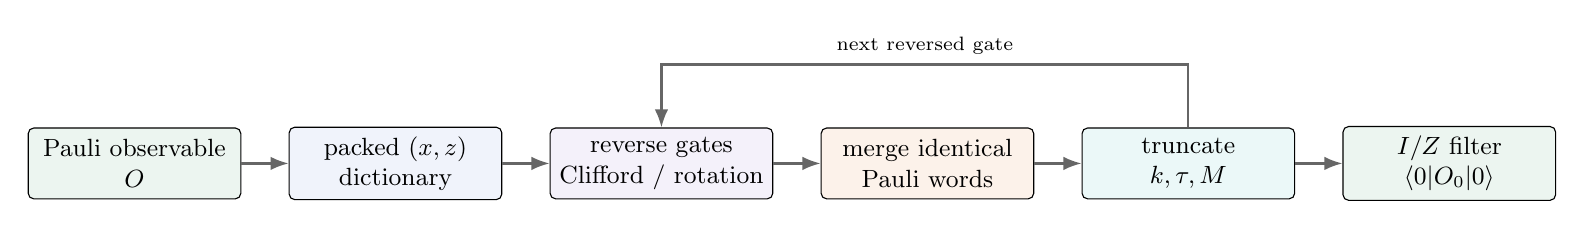
\begin{tikzpicture}[
  font=\small,
  box/.style={draw,rounded corners=2pt,minimum height=9mm,minimum width=27mm,align=center},
  arrow/.style={-{Latex[length=2.3mm]},thick,draw=black!60},
  node distance=6mm
]
\node[box,fill=qaspgreen!9] (obs) {Pauli observable\\$O$};
\node[box,fill=qaspblue!7,right=of obs] (pack) {packed $(x,z)$\\dictionary};
\node[box,fill=qasppurple!8,right=of pack] (prop) {reverse gates\\Clifford / rotation};
\node[box,fill=qasporange!10,right=of prop] (merge) {merge identical\\Pauli words};
\node[box,fill=qaspcyan!8,right=of merge] (prune) {truncate\\$k,\tau,M$};
\node[box,fill=qaspgreen!9,right=of prune] (zero) {$I/Z$ filter\\$\langle0|O_0|0\rangle$};
\foreach \a/\b in {obs/pack,pack/prop,prop/merge,merge/prune,prune/zero}{\draw[arrow] (\a)--(\b);}
\coordinate (loopa) at ($(prune.north)+(0,8mm)$);
\coordinate (loopb) at ($(prop.north)+(0,8mm)$);
\draw[arrow] (prune.north) -- (loopa) --
  node[above,font=\scriptsize]{next reversed gate} (loopb) -- (prop.north);
\end{tikzpicture}
}
\caption{Pauli-propagation pipeline.  Clifford gates do not branch; anticommuting parameterized Pauli rotations can create two terms.  Periodic merging and truncation control the active operator representation.}
\label{fig:pp}
\end{figure}

\subsubsection{Fast and differentiable engines}

\code{FastTruncatedPauliProp} stores ordinary Python complex coefficients and converts tape parameters to floating-point numbers.  It is intended for fast evaluation or analysis where gradients are not required.  \code{DifferentiablePauliProp} stores scalar Torch tensors instead.  Its $\cos\theta$ and $\sin\theta$ branches stay attached to the autograd graph, so gradients propagate through every retained path.

\begin{qaspfeature}{\code{FastTruncatedPauliProp} and \code{DifferentiablePauliProp}}
Two packed-integer Heisenberg simulators expose the same truncated Pauli path
with different numerical contracts.  The fast engine targets evaluation and
diagnostics; the differentiable engine retains Torch coefficients so gradients
flow through the currently selected Pauli paths.  Both make weight,
coefficient, term-count, and pruning-cadence budgets explicit.
\end{qaspfeature}

Hard selection is necessarily non-smooth.  The differentiable engine computes $\tau$ and top-$M$ masks from detached coefficient magnitudes, then preserves the original tensors for selected terms.  Gradients therefore describe the currently retained path set; they do not differentiate the discrete event at which a term enters or leaves that set.  Weight-$k$ truncation is structural.  This distinction is important when interpreting an approximate training trajectory.

The controls remain independent: \code{pp\_prune=False} disables coefficient
pruning but does not disable \code{pp\_truncation}.  Thus there is no
straight-through estimator for a pruning mask, and differentiability of the
retained computation is not an accuracy or learning guarantee.

With $M_t$ active Pauli terms, a local Clifford update is $O(M_t)$ and a supported rotation creates at most $2M_t$ pre-merge terms.  The advertised benefit is consequently conditional: execution is attractive when $M_t$ remains bounded by locality, cancellations, or chosen truncation, and unattractive when operator growth fills the available term budget.  Exactness on the supported gate set is recovered only with no active weight, coefficient, or count truncation and enough memory to retain all generated terms.  Users should report $k$, $\tau$, $M$, pruning cadence, and an exact-reference convergence check.

\begin{lstlisting}[caption={The ten-qubit \code{PQDQN} configuration used for
the $k=2$ Pauli-propagation benchmark.  In \qasp{}, \code{"lightning.pp"} is a
logical backend selector, not a separately installed PennyLane-Lightning
device.},label={lst:pp}]
from qasp.rl import PQDQN

model = PQDQN(
    n_qubits=10, n_actions=2,
    ansatz="AngleAnsatz",
    ansatz_config={
        "n_layers": 4, "rotations": "YZ",
        "reuploading": True,
        "include_imprimitive": True,
        "imprimitive": "CNOT",
        "imprimitive_pattern": "ring",
        "include_final_imprimitive": True,
    },
    feature_map="AngleEmbedding",
    feature_map_config={
        "features": 10, "rotations": "Y",
        "input_scaling": True,
    },
    observables=[f"Z {i}" for i in range(10)],
    fc_layer=True, fc_bias=True,
    input_activation="tanh",
    batch_mode="sequential",
    device="lightning.pp", diff_method="backprop",
    pp_truncation=2,
    pp_prune=False, pp_topM=None, pp_tau=0.0,
).double()
\end{lstlisting}

The selector is available to observable--softmax policies, recursive-parity
logical moments, binary and multiclass expectation-readout classifiers, and
\code{PQDQN} Pauli readouts.  Gradients remain connected to circuit rotations,
trainable input scaling or neural embeddings, and any classical head.  The
current engine consumes scalar-angle tapes, so arbitrary leading batch
dimensions are evaluated sample by sample and stacked while preserving the
PyTorch graph; \code{batch\_mode="broadcast"} does not create native Pauli-engine
broadcasting.  Born-probability outputs and sparse diagonal projector
measurements remain outside this backend because it accepts Pauli expectations,
not probability vectors or general sparse matrices.  This is an interface
boundary, not an approximation of their semantics.

\subsubsection{Ten-qubit PQDQN simulator microbenchmark}
\label{sec:pqdqn-pp-benchmark}

We benchmarked the model in \cref{lst:pp,fig:pqdqn-pp-circuit}: ten qubits,
four reuploaded $R_Y/R_Z$ ansatz layers, trainable $R_Y$ input scaling, a CNOT
ring in every layer including the final layer, and ten shared expectations
$z_i=\langle Z_i\rangle$ followed by the biased two-output head
$\bm Q=W\bm z+\bm b$.  The model has 142 trainable parameters.  Five matched
parameter initializations and normal input batches use seeds 7--11; QASP's
\code{normal\_0\_1} initializer means $\mathcal N(0,1)$, not standard deviation
$0.1$.  Each saved parameter state and input tensor is identical between the
exact \code{lightning.qubit}/adjoint reference and the two
\code{lightning.pp}/backprop approximations.

The Pauli runs set $k\in\{2,3\}$ with \code{pp\_prune=False},
\code{pp\_topM=None}, and \code{pp\_tau=0}; thus only Pauli-weight truncation is
active.  Both backends evaluate samples sequentially in CPU float64.  For each
seed, batch size, backend, and workload, two warmups precede seven timed
repeats, with backend order shuffled inside every repeat.  Torch intra- and
inter-op counts and OMP/OpenBLAS/MKL counts are fixed to one.  Measurements
were collected in one local session on an Apple M1 with 16 GiB memory and eight
hardware cores, without core pinning or thermal control.

\begin{table}[H]
\centering
\caption{Ten-qubit PQDQN timings in milliseconds per complete batch.  Entries
are mean $\pm$ sample SD of five within-seed medians, each based on seven timed
measurements after two warmups; the SD is descriptive, not a confidence
interval.}
\label{tab:pqdqn-pp-timing}
\small
\begin{tabular}{@{}r l r r@{}}
\toprule
Batch & Backend & Inference & Forward + backward \\
\midrule
1 & Lightning adjoint & $26.90\pm7.44$ & $28.59\pm5.45$ \\
1 & PP $k=2$          & $13.89\pm4.27$ & $16.69\pm1.87$ \\
1 & PP $k=3$          & $30.87\pm8.15$ & $48.24\pm10.12$ \\
8 & Lightning adjoint & $190.47\pm27.71$ & $198.02\pm9.00$ \\
8 & PP $k=2$          & $83.18\pm7.53$ & $110.29\pm8.16$ \\
8 & PP $k=3$          & $215.66\pm28.74$ & $326.91\pm30.35$ \\
\bottomrule
\end{tabular}
\end{table}

The forward--backward workload consists of \code{zero\_grad}, one complete
PQDQN call, a selected-action mean Huber loss, and \code{backward}.  It uses
fixed alternating actions and targets linearly spaced from $0.25$ to $1.75$;
optimizer updates, replay sampling, target-network evaluation, and environment
interaction are excluded.  It is therefore the differentiable kernel of a
Q-learning update, not a full DQN step or a learning curve.

For batch eight, $k=2$ is approximately $1.80\times$ faster than Lightning for
this gradient workload, while $k=3$ is slower.  Timing alone is misleading:
the batch-eight feature RMSE is $0.03164$ for both cutoffs and Q-value RMSE is
about $0.0176$, yet feature relative $\ell_2$ errors are $0.9984$ and $0.9973$.
The quantum-gradient relative $\ell_2$ errors are $1.0002$ and $0.9991$, with
cosine similarities $-0.015$ and $0.037$ for $k=2$ and $k=3$, respectively.
Quantum gradients include all circuit rotations and input scales but exclude
the classical head.  The small absolute Q-value errors therefore do not imply
accurate quantum propagation: the shared bias is unchanged and the affine
head can attenuate discarded-feature errors.

\begin{figure*}[p]
\centering
\begin{subfigure}{0.98\textwidth}
  \centering
  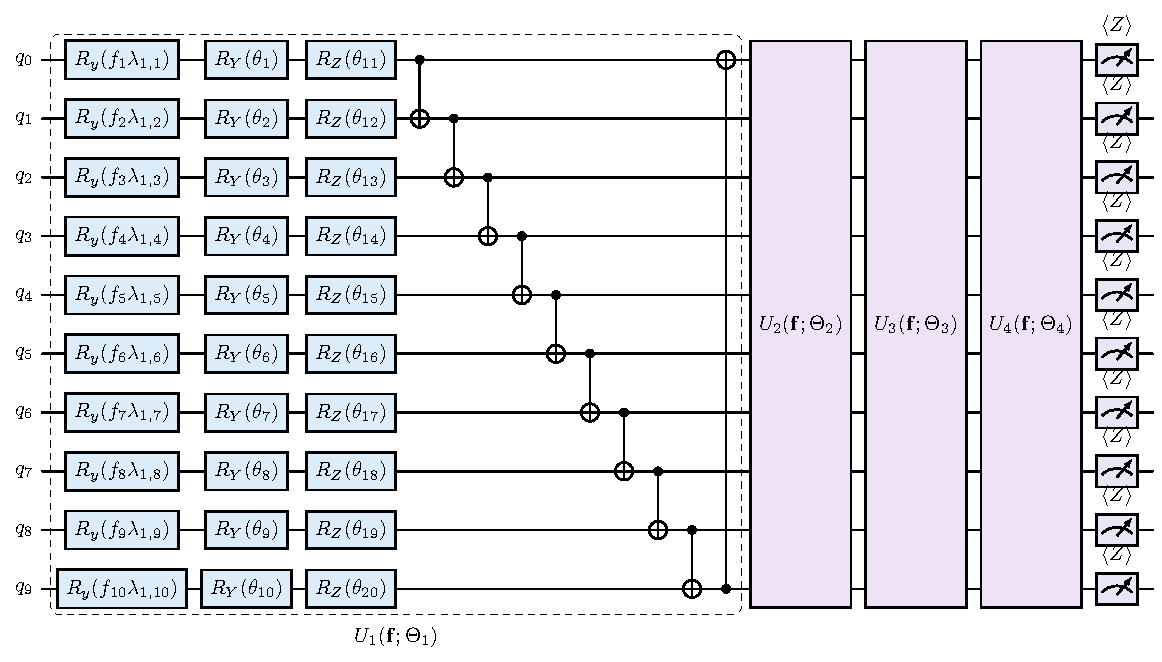
\includegraphics[width=0.98\textwidth]{figures/pqdqn_pp_10q_circuit.pdf}
  \caption{Compact Quantikz export of the common circuit.  The first complete
  layer is expanded and the remaining reuploaded layers are compressed.  The
  ten meters denote separate local-$Z$ expectations; $W\bm z+\bm b$ is
  classical and lies outside the circuit.}
  \label{fig:pqdqn-pp-circuit}
\end{subfigure}

\vspace{4mm}
\begin{subfigure}{0.92\textwidth}
  \centering
  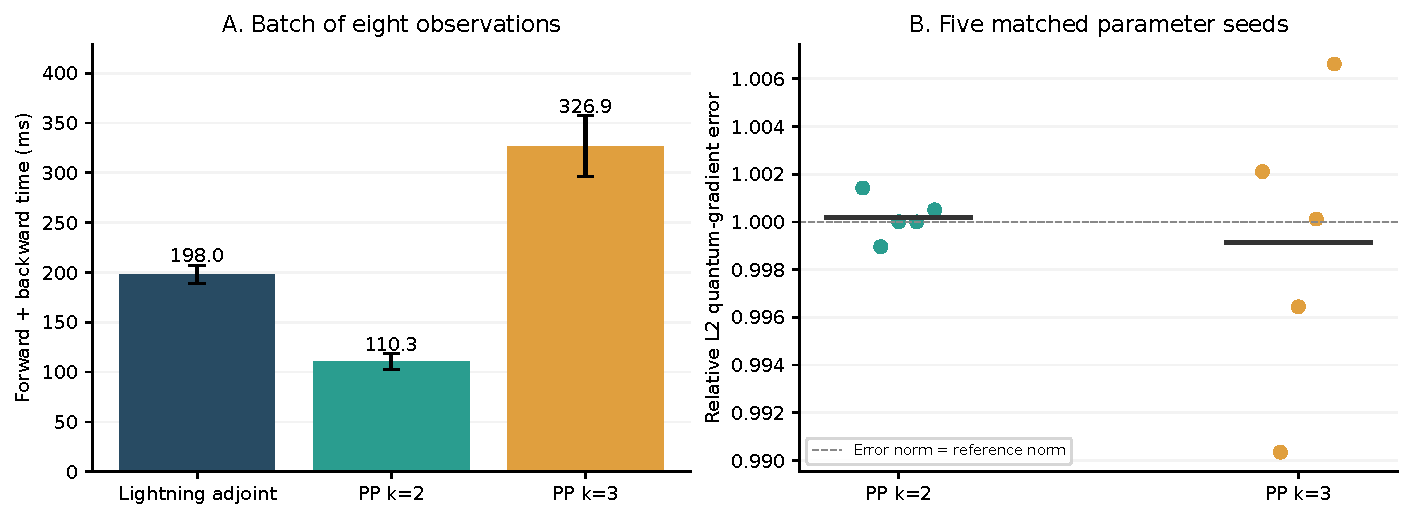
\includegraphics[width=\textwidth]{figures/pqdqn_pp_10q_timing_accuracy.pdf}
  \caption{Batch-eight forward--backward timing and per-seed quantum-gradient
  relative $\ell_2$ error.  Timing bars show mean $\pm$ sample SD across five
  seed medians; gradient dots are the five matched model seeds and horizontal
  marks are their means.  Error bars are not confidence intervals.}
  \label{fig:pqdqn-pp-timing-accuracy}
\end{subfigure}
\caption{Ten-qubit PQDQN simulator microbenchmark.  Low-weight propagation
exposes a runtime--accuracy trade-off: the faster $k=2$ measurement has
gradient error comparable to the norm of the exact gradient, while $k=3$ is
slower than the exact reference in this setup.}
\label{fig:pqdqn-pp-benchmark}
\end{figure*}

The exact Lightning result and all parameter gradients agree with
\code{default.qubit}/backprop for seed 7 and batch eight, with maximum gradient
discrepancy $2.52\times10^{-10}$.  Directional finite differences separately
confirm the derivative of each truncated Pauli function.  These checks verify
differentiation of the respective exact or truncated functions; they do not
make truncation exact.  The experiment provides no evidence of equivalent or
faster RL learning, accuracy-preserving speedup, asymptotic scalability, or
universal backend superiority.  Five parameter seeds are also not five
independent machine sessions.

\subsection{Distributed workload planning and execution}
\label{sec:hpc-planning}

The \code{qasp.hpc} package separates resource planning from execution.
\code{inspect\_workload} reads supported configurations, builders, or models
without constructing a large simulator or invoking user callbacks; explicit
\code{MemoryHints} fill dimensions that cannot be inferred safely.
\code{plan\_deucalion} then estimates state-vector storage, differentiation
storage, and replicated outputs and chooses a placement for one experiment or
independent repetitions.  These values are conservative analytical estimates
based on the documented 12 October 2026 machine profile.  They are neither
measured peak memory nor runtime guarantees, and host-memory, accelerator-
memory, and Slurm-memory units must not be conflated.

\begin{qaspfeature}{\code{inspect\_workload}, \code{plan\_deucalion}, and \code{render\_slurm}}
The HPC layer turns a QASP workload description into an inspectable resource
plan and a reproducible Slurm script.  Rendering never submits a job, copies
source code, or installs dependencies; \code{DeucalionJob.write} also refuses
to overwrite an existing file.  At runtime an \code{ExecutionContext} gives
callbacks their experiment index, MPI rank/world size, shared seed, and root-
rank status.  Every rank must enter a distributed simulation callback, while
ordinary artifact writing should be restricted to the root rank.
\end{qaspfeature}

Independent repetitions can be expressed as array or packed jobs; a single
distributed state vector instead occupies one MPI world.  QASP propagates the
requested backend and MPI options without silently falling back to serial
execution, so the installed PennyLane plugin and system MPI stack remain part
of the experiment contract.  The generated script is consequently a plan that
must still be submitted and monitored by the user or site scheduler.

% Show the detailed RL hierarchy in the contents without expanding every
% other module to the same depth.
\addtocontents{toc}{\protect\setcounter{tocdepth}{3}}
\section{Reinforcement learning}
\label{sec:rl}

\qasp{} supports two complementary reinforcement-learning contracts.  In
policy-based RL, the quantum model returns logits or normalized action
probabilities and is optimized directly through REINFORCE, AWR, or PPO.  In
value-based RL, it returns unconstrained action values and is optimized from
Bellman targets through deep Q-learning.  In both cases the quantum component
remains orthogonal to environment interaction, experience collection, and
classical optimizer state.  \Cref{fig:rl-loop} shows the policy-based path.

\begin{qaspfeature}{High-level RL modules}
\code{create\_model} specializes the common feature-map, ansatz, builder, and
backend stack as either \code{PQCSoftmax} or a decoded-Born model.  The factory
selector \code{"PQCBorn"} currently constructs the enhanced
\code{PQCBornVariance}; direct \code{PQCBorn} is a distinct legacy
sample-and-log-probability interface.  \code{create\_qfunction} builds the
value-based \code{PQDQN} counterpart.  Each maintained object is an ordinary
PyTorch module, but trainers must honor its logits, probabilities, or
unconstrained-Q-value contract.
\end{qaspfeature}

\subsection{Policy-based reinforcement learning}
\label{sec:rl-policy-based}

Policy-based agents parameterize the behavior distribution itself.  QASP
separates the quantum circuit, action readout, and classical learning rule so
that observable--softmax and decoded-Born policies can share the same rollout
and optimization infrastructure.  This subsection first fixes the policy
semantics and execution contracts, then presents the maintained trainers,
benchmarks, diagnostics, and circuit-export workflow.

\begin{figure*}[t]
\centering
\resizebox{\textwidth}{!}{%
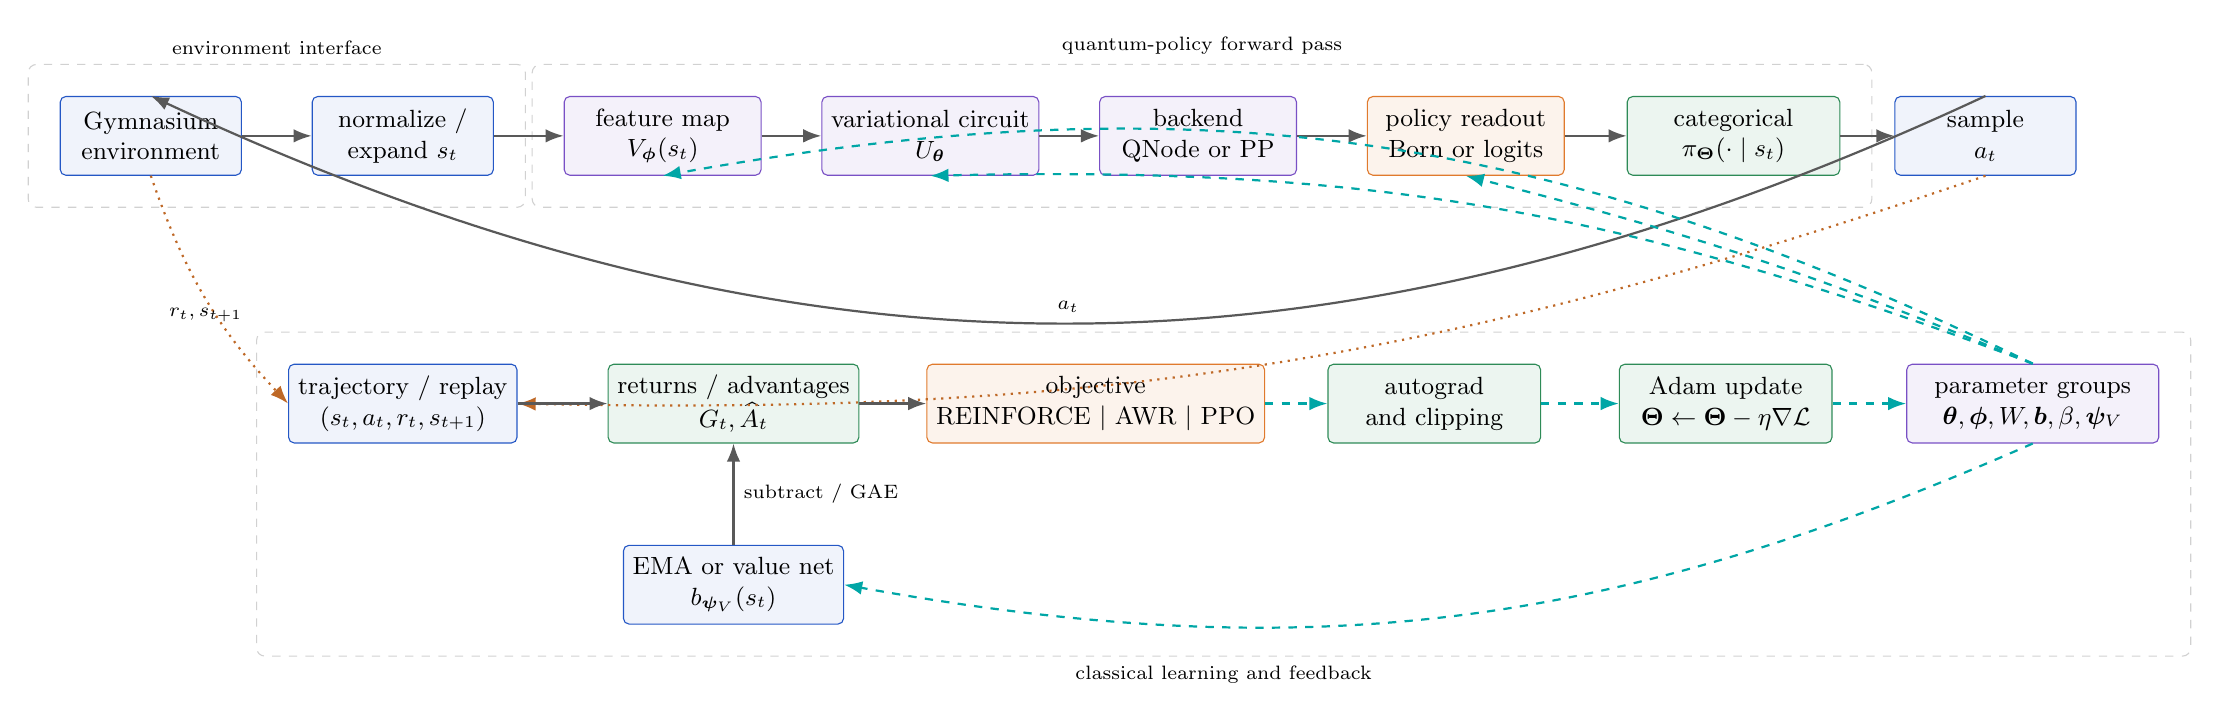
\begin{tikzpicture}[
  font=\small,
  box/.style={draw,rounded corners=2pt,minimum height=10mm,align=center,fill=white},
  envbox/.style={box,draw=qaspblue,fill=qaspblue!7,minimum width=23mm},
  qbox/.style={box,draw=qasppurple,fill=qasppurple!8,minimum width=25mm},
  rbox/.style={box,draw=qasporange,fill=qasporange!9,minimum width=25mm},
  lbox/.style={box,draw=qaspgreen,fill=qaspgreen!9,minimum width=27mm},
  arrow/.style={-{Latex[length=2.3mm]},thick,draw=black!65},
  data/.style={-{Latex[length=2.3mm]},thick,dotted,draw=qasporange!85!black},
  grad/.style={-{Latex[length=2.3mm]},thick,dashed,draw=qaspcyan},
  group/.style={draw=black!18,dashed,rounded corners=3pt,inner sep=4mm}
]
\node[envbox] (env) at (0,2.2) {Gymnasium\\environment};
\node[envbox] (prep) at (3.2,2.2) {normalize /\\expand $s_t$};
\node[qbox] (fm) at (6.5,2.2) {feature map\\$V_{\bm\phi}(s_t)$};
\node[qbox] (pqc) at (9.9,2.2) {variational circuit\\$U_{\bm\theta}$};
\node[qbox] (execute) at (13.3,2.2) {backend\\QNode or PP};
\node[rbox] (readout) at (16.7,2.2) {policy readout\\Born or logits};
\node[lbox] (dist) at (20.1,2.2) {categorical\\$\pi_{\bm\Theta}(\cdot\mid s_t)$};
\node[envbox] (action) at (23.3,2.2) {sample\\$a_t$};

\node[envbox,minimum width=29mm] (buffer) at (3.2,-1.2) {trajectory / replay\\$(s_t,a_t,r_t,s_{t+1})$};
\node[lbox,minimum width=29mm] (adv) at (7.4,-1.2) {returns / advantages\\$G_t,\widehat A_t$};
\node[rbox,minimum width=34mm] (objective) at (12.0,-1.2) {objective\\REINFORCE $\mid$ AWR $\mid$ PPO};
\node[lbox,minimum width=27mm] (autograd) at (16.3,-1.2) {autograd\\and clipping};
\node[lbox,minimum width=27mm] (optim) at (20.0,-1.2) {Adam update\\$\bm\Theta\leftarrow\bm\Theta-\eta\nabla\mathcal L$};
\node[qbox,minimum width=32mm] (params) at (23.9,-1.2) {parameter groups\\$\bm\theta,\bm\phi,W,\bm b,\beta,\bm\psi_V$};
\node[envbox,minimum width=27mm] (baseline) at (7.4,-3.5) {EMA or value net\\$b_{\bm\psi_V}(s_t)$};

\foreach \a/\b in {env/prep,prep/fm,fm/pqc,pqc/execute,execute/readout,readout/dist,dist/action}{\draw[arrow] (\a)--(\b);}
\draw[arrow,bend left=25] (action.north) to node[above,font=\scriptsize]{$a_t$} (env.north);
\draw[data] (env.south) to[bend right=12] node[below,font=\scriptsize]{$r_t,s_{t+1}$} (buffer.west);
\draw[data] (action.south) to[bend left=10] (buffer.east);
\draw[arrow] (buffer) -- (adv);
\draw[arrow] (adv) -- (objective);
\draw[grad] (objective) -- (autograd);
\draw[grad] (autograd) -- (optim);
\draw[grad] (optim) -- (params);
\draw[arrow] (baseline) -- node[right,font=\scriptsize]{subtract / GAE} (adv);
\draw[grad] (params.north) to[bend right=18] (fm.south);
\draw[grad] (params.north) to[bend right=11] (pqc.south);
\draw[grad] (params.north) to[bend right=4] (readout.south);
\draw[grad] (params.south) to[bend left=17] (baseline.east);

\begin{scope}[on background layer]
  \node[group,fit=(env)(prep),label={[font=\scriptsize]above:environment interface}] {};
  \node[group,fit=(fm)(pqc)(execute)(readout)(dist),label={[font=\scriptsize]above:quantum-policy forward pass}] {};
  \node[group,fit=(buffer)(adv)(objective)(autograd)(optim)(params)(baseline),label={[font=\scriptsize]below:classical learning and feedback}] {};
\end{scope}
\end{tikzpicture}
}
\caption{Detailed \qasp{} policy-based reinforcement-learning dataflow.  Solid arrows form the online interaction path, dotted orange arrows record experience, and dashed cyan arrows carry differentiable feedback.  The circuit and backend are isolated inside the policy forward pass, while state processing, sampling, returns/advantages, baselines, objective selection, and optimization remain classical and independently replaceable.}
\label{fig:rl-loop}
\end{figure*}
\subsubsection{Policy and action-readout primitives}
\label{sec:policies}

QRL connects a quantum state model to a classical Markov decision process.
For state $s$ and discrete action set $\A=\{0,\ldots,A-1\}$, \qasp{}
separates two questions that are easily conflated: \emph{what action does a
measurement outcome mean?} and \emph{how is the corresponding probability
evaluated and differentiated?}  This separation is the organizing principle
of the current RL policy implementation.

\paragraph{Observable--softmax policies.}

For Pauli observables $O_1,\ldots,O_q$, \code{PQCSoftmax} evaluates the
quantum feature vector
\begin{equation}
  \bm{z}_{\bm{\theta},\bm{\phi}}(s)
  = \big(\langle O_1\rangle_s,\ldots,\langle O_q\rangle_s\big).
  \label{eq:quantum-feature-vector}
\end{equation}
If $q=A$, these values may be used directly as action logits.  Alternatively,
a trainable classical head $W\in\R^{A\times q}$ and $\bm b\in\R^A$ produces
\begin{equation}
  \pi_{\bm{\Theta}}(a\mid s)
  = \operatorname{softmax}\!\left(
      \beta\left[W\bm{z}_{\bm{\theta},\bm{\phi}}(s)+\bm b\right]
    \right)_a,
  \quad
  \bm{\Theta}=(\bm{\theta},\bm{\phi},W,\bm b,\beta),
  \label{eq:softmax_policy}
\end{equation}
where $\beta$ is an optional fixed or trainable inverse-temperature scale.
The class returns scores from \code{forward}; a trainer must therefore use
\code{Categorical(logits=...)}.  Signed expectation values are never silently
reinterpreted as probabilities.  In the current constructor only
\code{fc\_layer=None} disables the affine head; any other value, including
\code{False}, creates it.  Its bias is trainable.  The older
\code{action\_probs()} shortcut bypasses that head, trainable scaling, and the
Pauli-propagation route, so logits-aware training should call \code{forward}.

\begin{qaspfeature}{\code{PQCSoftmax}}
An observable-based policy module whose quantum circuit returns Pauli
expectation features.  It exposes those features directly as action logits or
passes them through a trainable classical head and optional inverse
temperature.  Its explicit logits contract makes it compatible with standard
PyTorch categorical sampling and policy-gradient trainers.  The legacy
\code{action\_probs()} shortcut is not equivalent when the head, scaling, or
Pauli backend is active.
\end{qaspfeature}

\paragraph{One decoded-Born semantics.}

Let $M=(w_1,\ldots,w_m)$ be the ordered measured wires and
$z\in\{0,1\}^m$ a computational-basis outcome in PennyLane's big-endian
ordering.  A Born circuit defines
\begin{equation}
  p_{\bm{\theta},\bm{\phi}}(z\mid s)
  = \left|\langle z\mid
      \psi_{\bm{\theta},\bm{\phi}}(s)\rangle\right|^2.
  \label{eq:basis-born-probability}
\end{equation}
A deterministic decoder $d:\{0,1\}^m\rightarrow\A$ induces the action
projectors and policy
\begin{align}
  \Pi_a
  &=\sum_{z:\,d(z)=a}\lvert z\rangle\!\langle z\rvert,
  \label{eq:action-projector}\\
  \pi_{\bm{\theta},\bm{\phi}}(a\mid s)
  &=\langle\psi_{\bm{\theta},\bm{\phi}}(s)\rvert
    \Pi_a
    \lvert\psi_{\bm{\theta},\bm{\phi}}(s)\rangle
   =\sum_{z:\,d(z)=a}p_{\bm{\theta},\bm{\phi}}(z\mid s).
  \label{eq:born_policy}
\end{align}
Equivalently, with $D_{az}=\mathbf 1[d(z)=a]$, one has
$\bm\pi=D\bm p$ and $\sum_aD_{az}=1$ for every basis state.  The internal
\code{\_PolicyDecoder} precomputes the integer action index for all $2^m$
basis states.  Its forward path uses a batch-preserving Torch
\code{scatter\_add\_}; its sample path converts measured bits to the same
big-endian index and performs a lookup.  Consequently the implementation
enforces the semantic invariant
\begin{equation}
  \Pr_{Z\sim p}\!\left[\code{decode\_samples}(Z)=a\right]
  =\sum_zD_{az}p(z)=\pi(a\mid s),
  \label{eq:decoder-invariant}
\end{equation}
rather than maintaining separate, potentially inconsistent formulas for
training and deployment.

\begin{qaspfeature}{\code{PQCBorn} and \code{PQCBornVariance}}
High-level decoded-Born policies with one cached outcome-to-action map shared
by exact probability aggregation and sampled-action decoding.
\code{PQCBornVariance} additionally exposes the full-probability,
logical-moment, and sparse-projector execution contracts behind the same
normalized action distribution, so a backend can change without redefining
the policy.
\end{qaspfeature}

\paragraph{Decoder families.}

Release \version{} exposes four related outcome-to-action maps.  Write
$J(z)=\sum_{i=1}^{m}2^{m-i}z_i$ and
$k=\lceil\log_2A\rceil$.

\paragraph{Contiguous.}
Let $2^m=qA+r$, $0\leq r<A$, and let
$b_a=q+\mathbf 1[a<r]$.  Consecutive basis indices are assigned to action
$a$ whenever
\begin{equation}
  \sum_{j<a}b_j\leq J(z)<\sum_{j\leq a}b_j.
  \label{eq:contiguous-decoder}
\end{equation}
Thus the bins differ in size by at most one even when $A$ is not a power of
two, following the contiguous-policy construction of
\citet{jerbi2021policies}.

\paragraph{Recursive parity.}
The $k$ logical bits are nested prefix parities
\begin{equation}
  r_j(z)=z_1\oplus\cdots\oplus z_{m-j},
  \qquad j=0,\ldots,k-1,
  \label{eq:recursive-parity-bits}
\end{equation}
and the decoded action is
\begin{equation}
  d_{\mathrm{RP}}(z)
  =\left(\sum_{j=0}^{k-1}2^{k-1-j}r_j(z)\right)\bmod A.
  \label{eq:recursive-parity-decoder}
\end{equation}
This generalizes the binary global-parity readout and implements the optimized
action-decoding idea of \citet{Meyer2023ActionDecoding}.  The
\code{hidden-like} variant first selects a reduced ordered wire set---every
second circuit wire by default---and applies the same recursive map.

\paragraph{Majority--modulo.}
Let $B_0,\ldots,B_{k-1}$ be disjoint blocks of positions in the measured
bit string.  Define
\begin{equation}
  h_j(z)=\mathbf 1\!\left[
    \sum_{i\in B_j}z_i>\left\lfloor\frac{|B_j|}{2}\right\rfloor
  \right],
  \qquad
  d_{\mathrm{MM}}(z)
  =\left(\sum_{j=0}^{k-1}2^{k-1-j}h_j(z)\right)\bmod A.
  \label{eq:majority-modulo-decoder}
\end{equation}
The strict inequality gives deterministic tie-to-zero behavior for an
explicit even block.  If blocks are omitted, \qasp{} uses as many measured
wires as possible in positive odd blocks whose sizes differ by at most two,
leaving at most one wire unused.  The current strict option additionally
requires equal block sizes of at least three and no unused measured wire;
users reproducing the tie-free theoretical setting should choose that common
size to be odd.  Blocks are specified by actual device-wire labels, while the
decoder stores their positions in the ordered measurement register.

\begin{figure*}[t]
\centering
\resizebox{0.96\textwidth}{!}{%
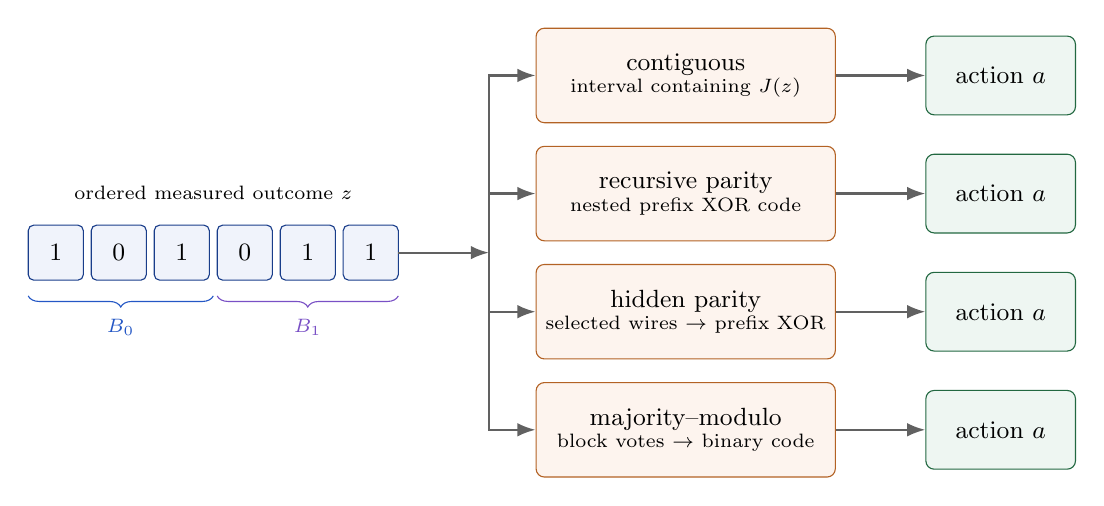
\begin{tikzpicture}[
  font=\small,
  bit/.style={draw=qaspblue!70!black,rounded corners=2pt,fill=qaspblue!7,
              minimum width=7mm,minimum height=7mm,align=center},
  map/.style={draw=qasporange!80!black,rounded corners=3pt,fill=qasporange!8,
              minimum width=38mm,minimum height=12mm,align=center},
  actionbox/.style={draw=qaspgreen!75!black,rounded corners=3pt,fill=qaspgreen!8,
              minimum width=19mm,minimum height=10mm,align=center},
  arrow/.style={-{Latex[length=2.3mm]},thick,draw=black!62}
]
\foreach \x/\b in {0/1,0.8/0,1.6/1,2.4/0,3.2/1,4.0/1}{
  \node[bit] at (\x,0) {$\b$};
}
\node[above,font=\scriptsize] at (2.0,0.55) {ordered measured outcome $z$};

\node[map] (cont) at (8.0,2.25)
  {contiguous\\[-1mm]\scriptsize interval containing $J(z)$};
\node[map] (par) at (8.0,0.75)
  {recursive parity\\[-1mm]\scriptsize nested prefix XOR code};
\node[map] (hidden) at (8.0,-0.75)
  {hidden parity\\[-1mm]\scriptsize selected wires $\rightarrow$ prefix XOR};
\node[map] (maj) at (8.0,-2.25)
  {majority--modulo\\[-1mm]\scriptsize block votes $\rightarrow$ binary code};
\node[actionbox] (a0) at (12.0,2.25) {action $a$};
\node[actionbox] (a1) at (12.0,0.75) {action $a$};
\node[actionbox] (a2) at (12.0,-0.75) {action $a$};
\node[actionbox] (a3) at (12.0,-2.25) {action $a$};
\coordinate (fork) at (5.5,0);
\draw[arrow] (4.35,0)--(fork);
\foreach \target in {cont,par,hidden,maj}{
  \draw[arrow] (fork) |- (\target.west);
}
\foreach \left/\right in {cont/a0,par/a1,hidden/a2,maj/a3}{
  \draw[arrow] (\left)--(\right);
}
\draw[decorate,decoration={brace,mirror,amplitude=4pt},qaspblue]
  (-0.35,-0.55)--(2.0,-0.55)
  node[midway,below=5pt,font=\scriptsize]{$B_0$};
\draw[decorate,decoration={brace,mirror,amplitude=4pt},qasppurple]
  (2.05,-0.55)--(4.35,-0.55)
  node[midway,below=5pt,font=\scriptsize]{$B_1$};
\end{tikzpicture}}
\caption{One measured bit string can support several explicit policy
semantics.  \qasp{} precomputes the selected map once and uses it for both
probability aggregation and sample decoding.  The majority braces are only an
illustrative block assignment; arbitrary disjoint measured-wire blocks may be
configured.}
\label{fig:decoder-families}
\end{figure*}

\paragraph{Four exact or differentiable execution contracts.}

The decoder fixes $\Pi_a$ and therefore the mathematical policy, but it does
not uniquely fix how that policy is evaluated.  \Cref{fig:decoder} shows the
four principal paths.

\begin{figure*}[t]
\centering
\resizebox{\textwidth}{!}{%
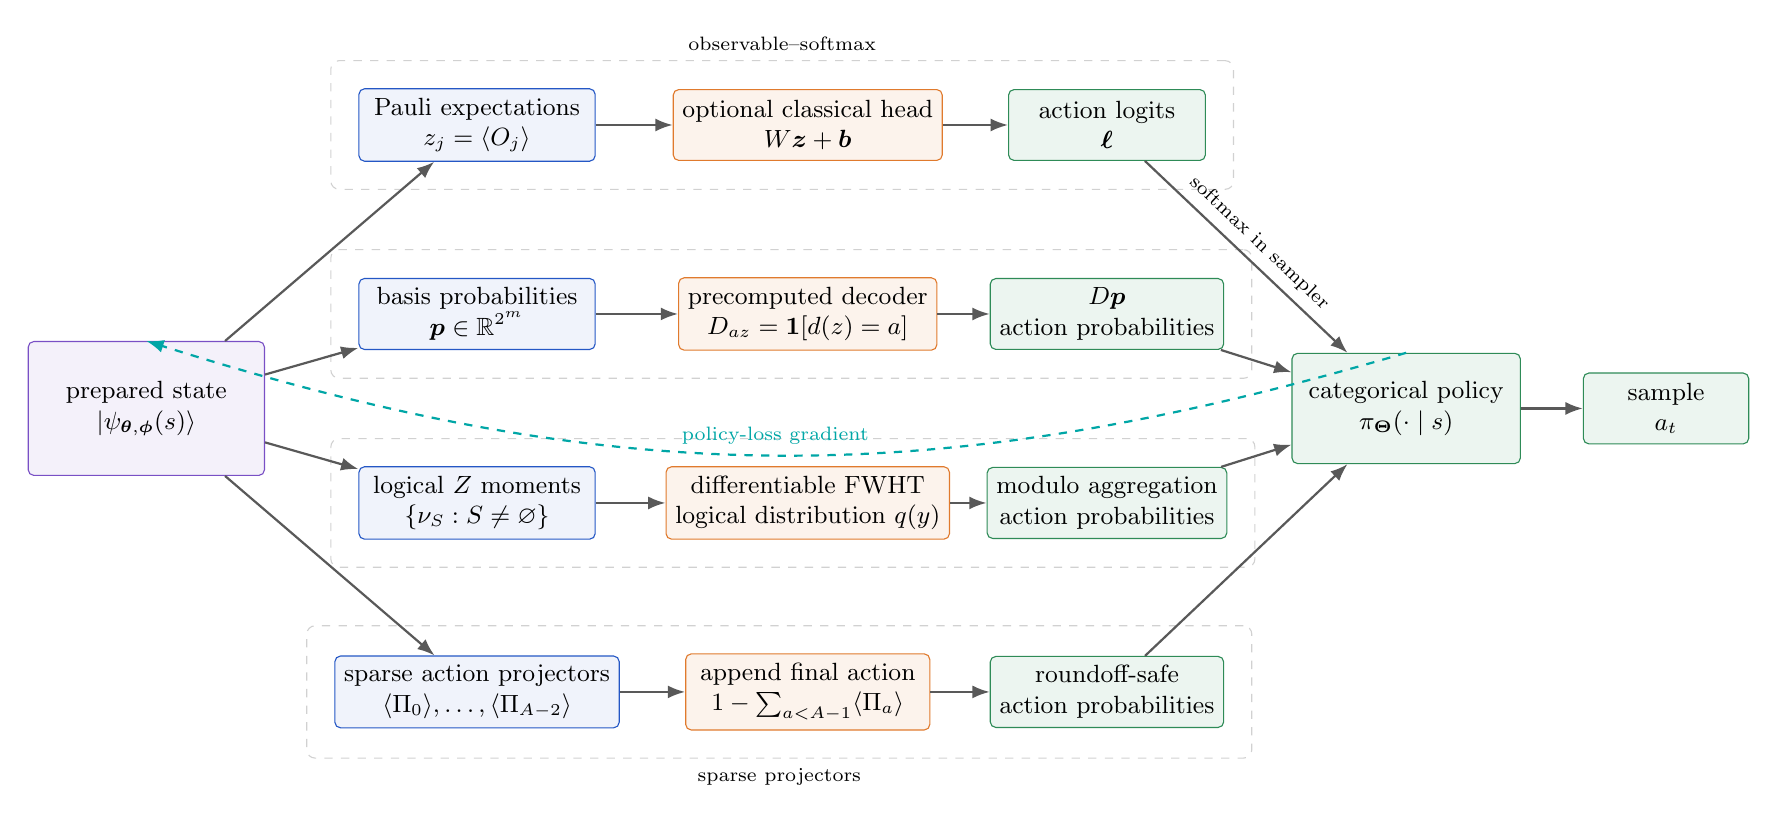
\begin{tikzpicture}[
  font=\small,
  box/.style={draw,rounded corners=2pt,minimum height=9mm,align=center,fill=white},
  quantum/.style={box,draw=qasppurple,fill=qasppurple!8},
  measure/.style={box,draw=qaspblue,fill=qaspblue!7,minimum width=30mm},
  decode/.style={box,draw=qasporange,fill=qasporange!9,minimum width=31mm},
  output/.style={box,draw=qaspgreen,fill=qaspgreen!9,minimum width=25mm},
  flow/.style={-{Latex[length=2.2mm]},thick,draw=black!65},
  grad/.style={-{Latex[length=2.2mm]},thick,dashed,draw=qaspcyan},
  lane/.style={draw=black!18,dashed,rounded corners=3pt,inner sep=3.5mm}
]
\node[quantum,minimum width=30mm,minimum height=17mm] (state) at (0,0)
  {prepared state\\$\lvert\psi_{\bm\theta,\bm\phi}(s)\rangle$};

\node[measure] (exp) at (4.2,3.6) {Pauli expectations\\$z_j=\langle O_j\rangle$};
\node[decode] (head) at (8.4,3.6) {optional classical head\\$W\bm z+\bm b$};
\node[output] (logits) at (12.2,3.6) {action logits\\$\bm\ell$};

\node[measure] (basis) at (4.2,1.2) {basis probabilities\\$\bm p\in\R^{2^m}$};
\node[decode] (decoder) at (8.4,1.2) {precomputed decoder\\$D_{az}=\mathbf 1[d(z)=a]$};
\node[output] (bornout) at (12.2,1.2) {$D\bm p$\\action probabilities};

\node[measure] (moments) at (4.2,-1.2) {logical $Z$ moments\\$\{\nu_S:S\ne\varnothing\}$};
\node[decode] (fwht) at (8.4,-1.2) {differentiable FWHT\\logical distribution $q(y)$};
\node[output] (modulo) at (12.2,-1.2) {modulo aggregation\\action probabilities};

\node[measure] (projector) at (4.2,-3.6) {sparse action projectors\\$\langle\Pi_0\rangle,\ldots,\langle\Pi_{A-2}\rangle$};
\node[decode] (residual) at (8.4,-3.6) {append final action\\$1-\sum_{a<A-1}\langle\Pi_a\rangle$};
\node[output] (sparseout) at (12.2,-3.6) {roundoff-safe\\action probabilities};

\node[output,minimum width=29mm,minimum height=14mm] (dist) at (16.0,0)
  {categorical policy\\$\pi_{\bm\Theta}(\cdot\mid s)$};
\node[output,minimum width=21mm] (action) at (19.3,0) {sample\\$a_t$};

\foreach \target in {exp,basis,moments,projector}{\draw[flow] (state) -- (\target);}
\foreach \left/\right in {exp/head,head/logits,basis/decoder,decoder/bornout,
                            moments/fwht,fwht/modulo,projector/residual,
                            residual/sparseout}{\draw[flow] (\left)--(\right);}
\draw[flow] (logits) -- node[above,sloped,font=\scriptsize]{softmax in sampler} (dist);
\draw[flow] (bornout) -- (dist);
\draw[flow] (modulo) -- (dist);
\draw[flow] (sparseout) -- (dist);
\draw[flow] (dist)--(action);
\draw[grad] (dist.north) to[bend left=17]
  node[above,font=\scriptsize,text=qaspcyan]{policy-loss gradient} (state.north);

\begin{scope}[on background layer]
  \node[lane,fit=(exp)(head)(logits),label={[font=\scriptsize]above:observable--softmax}] {};
  \node[lane,fit=(basis)(decoder)(bornout)] {};
  \node[lane,fit=(moments)(fwht)(modulo)] {};
  \node[lane,fit=(projector)(residual)(sparseout),label={[font=\scriptsize]below:sparse projectors}] {};
\end{scope}
\end{tikzpicture}}
\caption{Policy semantics and execution are separated.  The upper lane
constructs a softmax policy from quantum features.  The remaining lanes are
mathematically equivalent decoded-Born routes when their compatibility
conditions hold: full basis probabilities, logical-moment reconstruction, or
direct sparse action-projector expectations.}
\label{fig:decoder}
\end{figure*}

\paragraph{Full probabilities.}
With \code{training\_method="probs"}, the quantum layer returns all $2^m$
basis probabilities and the shared decoder computes $D\bm p$.  This path
supports every decoder and is the reference against which specialized paths
are tested, but its returned vector grows exponentially in the number of
measured wires.

\paragraph{Full $Z$-moment reconstruction.}
For compatible expectation devices, every basis probability can instead be
reconstructed from $2^m-1$ nonidentity moments
$\mu_t=\langle Z^t\rangle$, $t\in\{0,1\}^m$, by
\begin{equation}
  p(z)=2^{-m}\sum_{t\in\{0,1\}^{m}}(-1)^{t\cdot z}\mu_t,
  \qquad \mu_0=1.
  \label{eq:fwht}
\end{equation}
The PyTorch implementation stores the measurements in binary-mask order and
applies a differentiable fast Walsh--Hadamard transform (FWHT), preserving
arbitrary leading batch dimensions.

\paragraph{Logical-moment reconstruction for recursive parity.}
Recursive parity needs only the distribution of its $k$ logical bits, not the
full $m$-bit distribution.  Let
\begin{equation}
  R_j=\prod_{i=1}^{m-j}Z_{w_i},
  \qquad
  R_S=\prod_{j\in S}R_j,
  \qquad
  \nu_S=\langle R_S\rangle.
  \label{eq:logical-parity-observables}
\end{equation}
Repeated Pauli factors cancel, so the support of $R_S$ is the symmetric
difference of the nested prefix supports.  Measuring all
$2^k-1$ nonidentity $R_S$ yields the exact logical-code distribution
\begin{equation}
  q(y)=2^{-k}\sum_{S\subseteq\{0,\ldots,k-1\}}
       (-1)^{\sum_{j\in S}y_j}\nu_S,
  \qquad \nu_{\varnothing}=1,
  \label{eq:logical-fwht}
\end{equation}
after which
\begin{equation}
  \pi(a\mid s)=\sum_{y:\,J(y)\bmod A=a}q(y).
  \label{eq:logical-modulo}
\end{equation}
Thus the quantum output count depends on $A$ through
$2^{\lceil\log_2A\rceil}-1$, rather than on all $2^m$ measurement outcomes.
The same reconstruction applies when CNOT networks materialize the logical
parities on ancillas.  This exact multi-action path is regression-tested for
$A=3$ and $A=4$ against full probabilities and their parameter gradients.

\paragraph{Sparse majority action projectors.}
Majority projectors are generally dense in their Pauli--$Z$ Fourier expansion,
but diagonal in the computational basis.  \qasp{} therefore constructs each
$\Pi_a$ directly as a SciPy CSR diagonal matrix over all data and ancilla
wires.  With analytic execution,
\begin{equation}
  \pi(a\mid s)=\langle\Pi_a\rangle,
  \quad a=0,\ldots,A-2,
  \qquad
  \pi(A-1\mid s)=1-\sum_{a=0}^{A-2}\langle\Pi_a\rangle.
  \label{eq:sparse-residual}
\end{equation}
Only $A-1$ observables are evaluated.  Machine-precision negative residuals
are clamped and the vector is renormalized before construction of a
categorical distribution.

This path intentionally has a narrow contract: it uses analytic
\code{lightning.qubit} or \code{lightning.kokkos},
\code{diff\_method="adjoint"}, \code{device\_vjp=False}, and
\code{batch\_obs=False}.  The device-native vector--Jacobian product is
deliberately disabled because it produced incorrect gradients for three or
more sparse-projector measurements in the tested PennyLane-Lightning stack;
the standard adjoint path agrees with the full-probability reference.  Shots,
Kokkos MPI, circuit cutting, and \code{lightning.pp} are rejected for this
mode instead of silently substituting another policy.

\begin{table*}[t]
\centering
\caption{Decoded-Born execution contracts in the current implementation.
$m$ is the number of measured wires and $k=\lceil\log_2A\rceil$.  ``Exact''
describes the mathematical readout, not the scaling of its simulator.}
\label{tab:policy-execution-contracts}
\small
\begin{tabularx}{\textwidth}{@{}p{0.19\textwidth}p{0.19\textwidth}p{0.17\textwidth}X p{0.19\textwidth}@{}}
\toprule
Training method & Quantum outputs & Compatible decoders & Post-processing & Principal boundary \\
\midrule
\code{probs} & $2^m$ probabilities & all four families & vectorized scatter-add with cached action indices & exponential output vector \\
\code{expectation}, logical & $2^k-1$ Pauli moments & recursive parity & FWHT on logical bits, then modulo aggregation & expectation-compatible analytic or finite-shot device \\
\code{expectation}, full & $2^m-1$ Pauli moments & contiguous, hidden parity, and ancilla parity & full FWHT, then shared decoder & no output-count advantage over full probabilities \\
\code{sparse\_projectors} & $A-1$ sparse expectations & majority--modulo & append residual action and normalize roundoff & analytic Lightning adjoint; no device VJP, MPI, cutting, or PP \\
direct samples & one or batched $m$-bit strings & all four families & big-endian lookup through the same cached decoder & gradients require a separate estimator \\
\bottomrule
\end{tabularx}
\end{table*}

\paragraph{Adaptive measurement selection.}

\code{LearnablePQCBorn} records an experimental attempt to augment a Born
policy with a classical selector over $k$-wire measurement subsets.  Given an
observation, a linear softmax model samples a wire combination and appends it
to the adaptive circuit input.  The current setup and post-processing path has
known limitations, so the class is retained as a prototype rather than a
validated adaptive-measurement trainer.

\begin{qaspfeature}{\code{LearnablePQCBorn}}
A historical adaptive-measurement prototype in which a classical selector
chooses a measured-wire subset before quantum execution.  It requires further
integration work before it should be used for learning claims.
\end{qaspfeature}


\subsubsection{Policy contract at the trainer boundary}

All current RL trainers consume an ordinary \torch{} module.  The only
semantic distinction the trainer must know is whether \code{forward} returns
logits or probabilities: \code{PQCSoftmax} is passed as logits to a
\code{Categorical} distribution, whereas \code{PQCBornVariance} is passed as
probabilities.  The latter's \code{forward} and
\code{action\_probs} methods now share exactly the same decoding path.  This
small interface rule makes it possible to exchange full-probability,
logical-moment, and sparse-projector implementations without changing the
REINFORCE objective or environment interaction code.

Configuration reuse also requires care: classifier, kernel, and Q-function
factories copy their dictionaries, whereas the legacy policy factory performs
a shallow copy and may mutate nested component dictionaries.  Reusable policy
templates should therefore be deep-copied before construction.  Historical
policy weight setters may call a nonexistent QNode method; ordinary Torch
\code{state\_dict} loading is the supported transfer mechanism.

For one trajectory $\tau$, the score-function identity remains
\begin{equation}
  \nabla_{\bm\Theta}J
  =\E_{\tau\sim\pi_{\bm\Theta}}
   \left[\sum_t G_t\,
   \nabla_{\bm\Theta}\log\pi_{\bm\Theta}(a_t\mid s_t)\right].
  \label{eq:policy-gradient-identity}
\end{equation}
The quantum-specific work is therefore concentrated in producing a
normalized, differentiable $\bm\pi(s_t)$ and its log probability; trajectory
collection, baselines, advantage normalization, entropy bonuses, and optimizer
state remain classical.


\subsubsection{Windy Target Navigation}
\label{sec:windy-navigation}

The release adds \code{WindyTargetNavigationEnv}, a self-contained Gymnasium
benchmark designed around the current three- and four-action policies.  A point
mass moves through a sequence of randomly placed waypoints under inertia and a
persistent stochastic wind.  For $A\in\{3,4\}$, action $a$ selects an equally
spaced unit thrust direction
\begin{equation}
  \bm u_a=
  \left(\cos\frac{2\pi a}{A},\sin\frac{2\pi a}{A}\right).
  \label{eq:windy-action}
\end{equation}
With time step $\Delta t$, thrust $c$, drag $\delta$, speed bound $v_{\max}$,
wind persistence $\rho$, and Gaussian innovation $\bm\epsilon_t$, the update is
\begin{align}
  \widetilde{\bm v}_{t+1}
    &=\delta\bm v_t+\Delta t(c\bm u_{a_t}+\bm w_t),
  &\bm v_{t+1}&=\operatorname{clipnorm}_{v_{\max}}
                     (\widetilde{\bm v}_{t+1}),\nonumber\\
  \bm p_{t+1}&=\bm p_t+\Delta t\,\bm v_{t+1},
  &\bm w_{t+1}&=\operatorname{clip}_{[-w_{\max},w_{\max}]}
                    (\rho\bm w_t+\bm\epsilon_t).
  \label{eq:windy-dynamics}
\end{align}
The six-dimensional observation is
\begin{equation}
  s_t=\left[
  \tanh\!\left(\frac{\bm g_t-\bm p_t}{d_{\max}}\right),
  \operatorname{clip}\!\left(\frac{\bm v_t}{v_{\max}}\right),
  \operatorname{clip}\!\left(\frac{\bm w_t}{w_{\max}}\right)
  \right],
  \label{eq:windy-observation}
\end{equation}
where $\bm g_t$ is the active waypoint.  If
$d_t=\|\bm g_t-\bm p_t\|_2$, the shaped reward is
\begin{equation}
  R_t=4(d_t-d_{t+1})-0.02-0.01\|\bm v_{t+1}\|_2^2
      +3\,\mathbf 1_{\mathrm{waypoint}}
      +7\,\mathbf 1_{\mathrm{all\ waypoints}}.
  \label{eq:windy-reward}
\end{equation}
The task therefore rewards progress while penalizing time and excessive
velocity.  Episodes terminate after the configured number of waypoints or
truncate at the step limit.  The environment follows the Gymnasium reset/step
contract, bounds every observation in $[-1,1]^6$, and reproduces complete
trajectories under identical seeds.

\begin{qaspfeature}{\code{WindyTargetNavigationEnv}}
A seeded Gymnasium benchmark for three- and four-action quantum policies.  It
provides bounded six-dimensional observations, inertial waypoint dynamics,
persistent stochastic wind, shaped rewards, and reproducible reset/step
semantics without coupling the environment to a particular policy class.
\end{qaspfeature}

\begin{figure*}[t]
\centering
\resizebox{0.98\textwidth}{!}{%
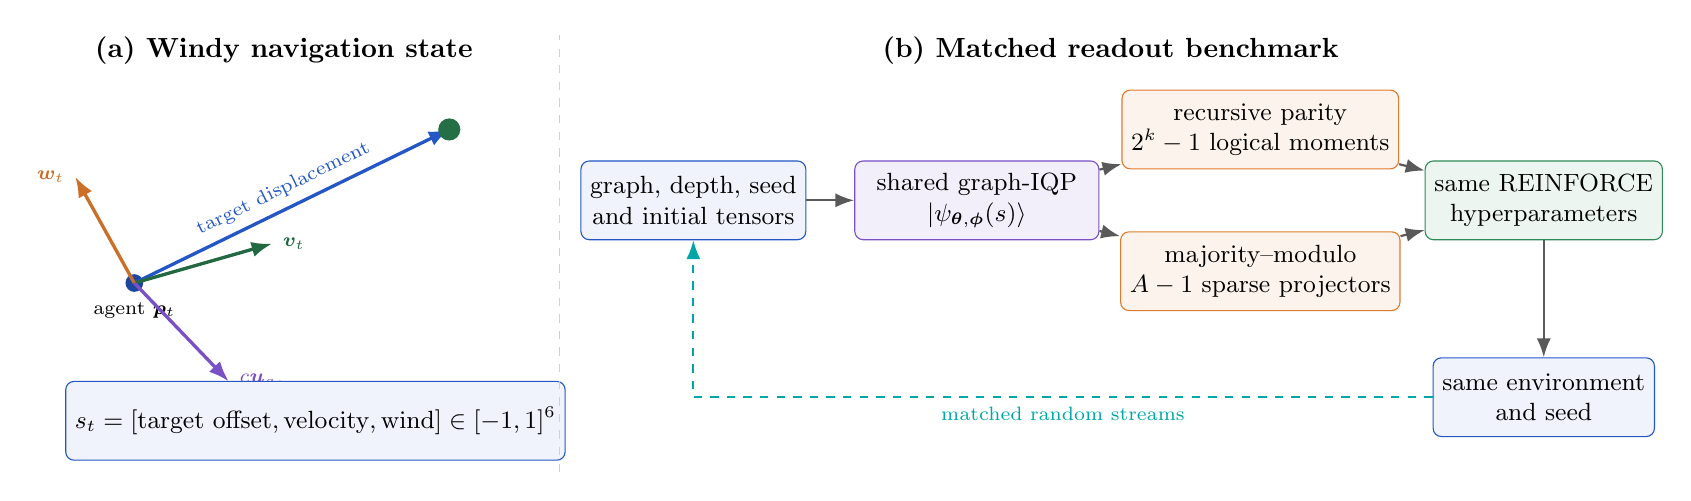
\begin{tikzpicture}[
  font=\small,
  box/.style={draw,rounded corners=3pt,minimum height=10mm,align=center},
  qbox/.style={box,draw=qasppurple,fill=qasppurple!9,minimum width=31mm},
  rbox/.style={box,draw=qasporange,fill=qasporange!9,minimum width=31mm},
  gbox/.style={box,draw=qaspgreen,fill=qaspgreen!9,minimum width=27mm},
  bbox/.style={box,draw=qaspblue,fill=qaspblue!7,minimum width=27mm},
  arrow/.style={-{Latex[length=2.4mm]},thick,draw=black!65},
  matched/.style={-{Latex[length=2.4mm]},thick,dashed,draw=qaspcyan}
]
\node[font=\bfseries] at (2.8,3.15) {(a) Windy navigation state};
\fill[qaspblue!80!black] (0.9,0.2) circle (3.2pt);
\node[below,font=\scriptsize] at (0.9,0.08) {agent $\bm p_t$};
\draw[qaspblue,very thick,-{Latex[length=2.6mm]}] (0.9,0.2)--(4.9,2.15)
  node[midway,above,sloped,font=\scriptsize] {target displacement};
\fill[qaspgreen!80!black] (4.9,2.15) circle (4pt);
\draw[qaspgreen!75!black,very thick,-{Latex[length=2.6mm]}]
  (0.9,0.2)--(2.65,0.7) node[right,font=\scriptsize] {$\bm v_t$};
\draw[qasporange!90!black,very thick,-{Latex[length=2.6mm]}]
  (0.9,0.2)--(0.15,1.55) node[left,font=\scriptsize] {$\bm w_t$};
\draw[qasppurple,very thick,-{Latex[length=2.6mm]}]
  (0.9,0.2)--(2.1,-1.05) node[right,font=\scriptsize] {$c\bm u_{a_t}$};
\node[bbox,minimum width=46mm] at (3.2,-1.55)
  {$s_t=[\text{target offset},\text{velocity},\text{wind}]\in[-1,1]^6$};

\draw[black!18,dashed] (6.3,-2.2)--(6.3,3.35);
\node[font=\bfseries] at (13.3,3.15) {(b) Matched readout benchmark};
\node[bbox] (spec) at (8.0,1.25) {graph, depth, seed\\and initial tensors};
\node[qbox] (iqp) at (11.6,1.25) {shared graph-IQP\\$\lvert\psi_{\bm\theta,\bm\phi}(s)\rangle$};
\node[rbox] (parity) at (15.2,2.15)
  {recursive parity\\$2^k-1$ logical moments};
\node[rbox] (majority) at (15.2,0.35)
  {majority--modulo\\$A-1$ sparse projectors};
\node[gbox] (trainer) at (18.8,1.25) {same REINFORCE\\hyperparameters};
\node[bbox] (environment) at (18.8,-1.25) {same environment\\and seed};
\draw[arrow] (spec)--(iqp);
\draw[arrow] (iqp)--(parity);
\draw[arrow] (iqp)--(majority);
\draw[arrow] (parity)--(trainer);
\draw[arrow] (majority)--(trainer);
\draw[arrow] (trainer)--(environment);
\draw[matched] (environment.west) -| (spec.south)
  node[pos=0.25,below,font=\scriptsize,text=qaspcyan]{matched random streams};
\end{tikzpicture}}
\caption{The new control benchmark and its intended comparison protocol.
(a) The observation exposes the relative target, velocity, and wind, while the
action chooses one of three or four thrust directions.  (b) Parity and
majority--modulo policies share the same graph-IQP circuit, initial trainable
tensors, environment seeds, and trainer settings; only the readout contract
changes.}
\label{fig:windy-and-matched-benchmark}
\end{figure*}

\subsubsection{Matched trainability-aware policy experiments}

The accompanying policy-efficiency notebook implements paired experiments in
which recursive-parity and majority--modulo policies receive exactly equal
trainable tensors for each circuit depth and seed.  The first readout uses the
logical-moment path; the second uses sparse projectors.  This pairing isolates
the policy decoder from initialization and circuit effects.

Two bounded-degree graph families are provided for the windy task: a fast
five-qubit chorded-cycle proxy and a seeded ten-qubit $3$-regular graph accepted
only when its adjacency spectral gap exceeds a configured threshold.  The
notebook spans $A\in\{3,4\}$ and repeated graph-IQP depths
$L\in\{1,2,3\}$.  For five qubits, the majority blocks
$\{0,1,2\}$ and $\{3\}$ avoid ties and leave wire $4$ active in the circuit but
unused by the classical decoder; for ten qubits, two blocks of five use every
measured wire.  The notebook first compares random actions with a feedback
controller, then records returns, success rates, runtimes, and matched
parameter checks.  These are benchmark protocols supplied by the release, not
performance claims in this software description; publishable numerical
comparisons must be regenerated from the final tag.

\subsubsection{Inspectable policy construction and circuit drawings}
\label{sec:rl-drawings}

The high-level factory does not hide the circuit it creates.  Every policy retains its resolved feature map, ansatz, builder, QNode, parameter shapes, and Torch layer.  The public \code{draw\_model} function traces that same executable circuit, including encoders, entangling topology, selected measurement wires, and parity ancillas.  With \code{output="tikz"}, it returns Quantikz source with symbolic feature, scaling, and circuit parameters.  This is useful both as a debugging check and as a reproducibility artifact: a paper figure can be generated from the experiment configuration rather than independently reconstructed in a graphics program.

\Cref{lst:draw-softmax} builds a compact observable--softmax policy for a four-dimensional observation and exports its circuit.  The four measured observables form the quantum feature vector; the final $4\times2$ classical head is outside the quantum circuit and consequently is described in the caption rather than drawn as a quantum gate.

\begin{lstlisting}[caption={Constructing and drawing an observable--softmax RL policy.  The saved circuit is shown in \cref{fig:rl-softmax-circuit}.},label={lst:draw-softmax}]
from pathlib import Path
import torch
from qasp import create_model, draw_model

n_qubits = 4
softmax_config = {
    "ansatz": "AngleAnsatz",
    "ansatz_config": {
        "n_layers": 2, "rotations": "ZY", "reuploading": False,
        "include_imprimitive": True, "imprimitive": "CZ",
        "imprimitive_pattern": "ring",
        "include_final_imprimitive": False,
        "include_feature_map_first": True,
        "include_hadamards_initial": True,
    },
    "feature_map": "NeuralEmbedding",
    "feature_map_config": {"features": 4, "rotations": "Z"},
    "n_actions": 2,
    "observables": ["Z 0", "Z 1", "ZZ 0 1", "ZZ 2 3"],
    "fc_layer": True,
    "init": "small_normal",
    "device": "default.qubit",
    "diff_method": "backprop",
}
softmax_policy = create_model(
    "PQCSoftmax", softmax_config, n_qubits=n_qubits
)
tikz = draw_model(
    model=softmax_policy, inputs=torch.zeros(4), output="tikz",
    tikz_options={
        "standalone": True, "symbolic_parameters": True,
        "compress": True,
    },
)
Path("figures").mkdir(exist_ok=True)
Path("figures/rl_softmax_observable.tex").write_text(tikz)
\end{lstlisting}

The corresponding Born construction in \cref{lst:draw-born} has the same circuit-level building blocks but a different measurement and action contract.  It measures the full computational-basis distribution and applies recursive parity only after quantum execution.  Thus the circuit drawing verifies the trainable model, while the separately reported decoder definition verifies how basis states become actions.

\begin{lstlisting}[caption={Constructing and drawing a Born parity policy.  The returned forward value is a normalized two-action probability vector and must be passed to \code{Categorical(probs=...)}.},label={lst:draw-born}]
from pathlib import Path
from qasp import create_model, draw_model
import torch

n_qubits = 4
parity_config = {
    "ansatz": "AngleAnsatz",
    "ansatz_config": {
        "n_layers": 2, "rotations": "ZY", "reuploading": False,
        "include_imprimitive": True, "imprimitive": "CZ",
        "imprimitive_pattern": "ring",
        "include_final_imprimitive": False,
        "include_feature_map_first": True,
        "include_hadamards_initial": True,
    },
    "feature_map": "AngleEmbedding",
    "feature_map_config": {
        "features": 4, "rotations": "Y", "input_scaling": True,
    },
    "n_actions": 2,
    "policy": "parity-like",
    "measurement_qubits": [0, 1, 2, 3],
    "training_method": "probs",
    "parity_cnot_decomposition": False,
    "init": "small_normal",
    "device": "default.qubit",
    "diff_method": "backprop",
}
parity_policy = create_model("PQCBorn", parity_config,
                             n_qubits=n_qubits)
action_probabilities = parity_policy(torch.zeros(4))
tikz = draw_model(
    model=parity_policy, inputs=torch.zeros(4), output="tikz",
    tikz_options={
        "standalone": True, "symbolic_parameters": True,
        "compress": True,
    },
)
Path("figures/rl_born_parity.tex").write_text(tikz)
\end{lstlisting}

\begin{figure*}[p]
\centering
\begin{subfigure}{0.98\textwidth}
  \centering
  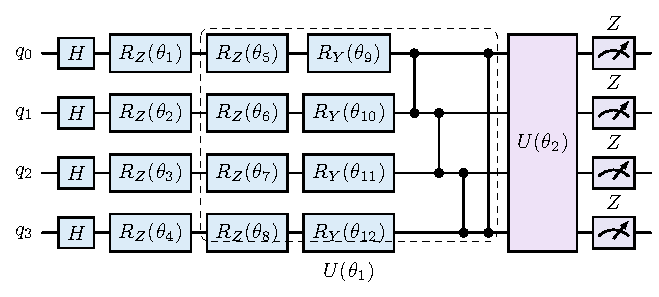
\includegraphics[width=\textwidth]{figures/rl_softmax_observable.pdf}
  \caption{Observable--softmax policy: trainable neural $Z$ encoding, one explicit $R_Z/R_Y$ ring-entangled layer, a compressed $U(\bm\theta_2)$ layer, four Pauli measurements, and a classical two-action head.}
  \label{fig:rl-softmax-circuit}
\end{subfigure}

\vspace{3mm}
\begin{subfigure}{0.98\textwidth}
  \centering
  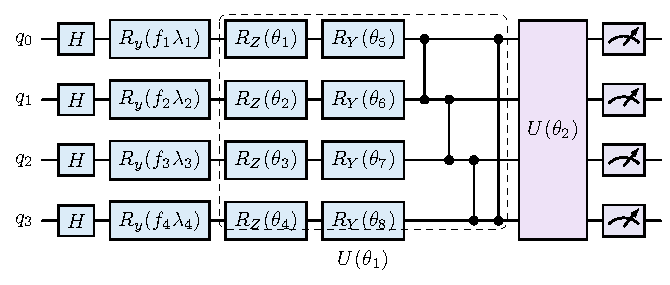
\includegraphics[width=\textwidth]{figures/rl_born_parity.pdf}
  \caption{Born parity policy: trainable angle scaling, one explicit variational layer, a compressed $U(\bm\theta_2)$ layer, full basis measurement, and an external fixed parity decoder.}
  \label{fig:rl-born-parity-circuit}
\end{subfigure}
\caption{Standard QASP reinforcement-learning readouts generated from the
executable policy objects with \qasp{}'s
\code{draw\_model(output="tikz")} path.  Symbolic parameters, semantic gate
colors, and repeated-layer compression are supplied by the exporter.  The
classical softmax head and fixed parity decoder are stated in the subcaptions
because they act after quantum measurement.}
\label{fig:rl-circuit-gallery}
\end{figure*}

\begin{figure*}[p]
\centering
\begin{subfigure}{0.98\textwidth}
  \centering
  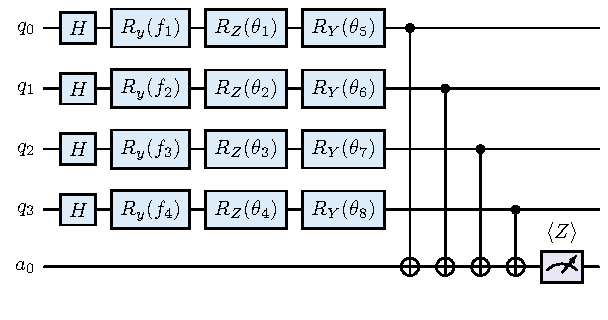
\includegraphics[width=0.84\textwidth]{figures/rl_ancilla_parity.pdf}
  \caption{Ancilla parity policy: four data wires fan into ancilla wire 4 with CNOTs; a single ancilla expectation represents the binary action readout.}
  \label{fig:rl-ancilla-circuit}
\end{subfigure}

\vspace{3mm}
\begin{subfigure}{0.98\textwidth}
  \centering
  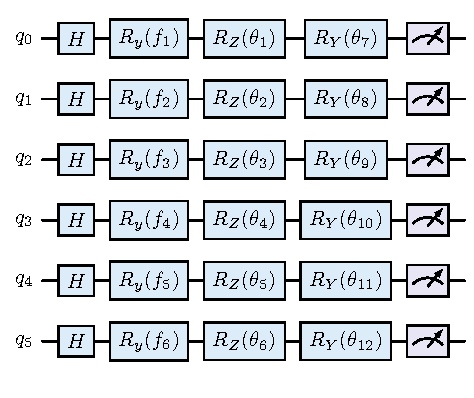
\includegraphics[width=0.74\textwidth]{figures/rl_majority_modulo.pdf}
  \caption{Three-action majority--modulo policy: six measured wires are decoded as odd blocks $\{0,1,2\}$ and $\{3,4,5\}$ after basis-probability evaluation.}
  \label{fig:rl-majority-circuit}
\end{subfigure}
\caption{Decoder-specialized QASP reinforcement-learning circuits generated
through the same Quantikz path.  The ancilla construction materializes parity
inside the circuit; majority--modulo keeps its deterministic action decoder
outside the measured circuit.  The companion \code{render\_rl\_circuits.py}
script retains editable standalone Quantikz and compiles the vector PDFs and
PNG previews used by the paper.}
\label{fig:rl-decoder-circuit-gallery}
\end{figure*}

\subsubsection{REINFORCE}

The primary \code{REINFORCE} trainer batches complete episodes.  With discounted return $G_t=\sum_{j\geq0}\gamma^jr_{t+j}$, baseline $b(s_t)$, and policy entropy $\Hc(\pi(\cdot\mid s_t))$, it minimizes
\begin{equation}
  \mathcal{L}_{\mathrm{PG}}
  =-\frac{1}{B}\sum_{\tau\in\mathcal{B}}\sum_{t\in\tau}
  \widehat{A}_t\log\pi_{\bm{\theta}}(a_t\mid s_t)
  -\beta_{\Hc}\Hc\!\left(\pi_{\bm{\theta}}(\cdot\mid s_t)\right),
  \label{eq:reinforce}
\end{equation}
where $\widehat{A}_t$ may be normalized across a batch.  Baselines are either an exponential moving average of returns or a small classical value network.  The trainer provides state scaling and nonlinear feature expansion, entropy regularization, episode batching, gradient clipping, and optional Acrobot reward shaping.  These controls are particularly relevant to PQCs because the basic score-function estimator already has high variance \cite{williams1992reinforce}.

The file also contains a configurable \code{Reinforce} implementation with
online observation normalization, mean-return or MLP baselines, evaluation
episodes, distinct learning-rate groups, and its own stopping rules.  It is a
different implementation, not an alias of the capitalized \code{REINFORCE}
top-level export.  The latter's CartPole-specific rule freezes optimization
once the available trailing window of at most 100 training returns reaches a
mean of 195; that implementation rule is not a \code{CartPole-v1} solved
certificate and does not replace held-out evaluation.

\begin{qaspfeature}{\code{REINFORCE}}
The top-level episode-batched policy-gradient trainer.  It accepts any QASP
policy module, selects logits or probability sampling explicitly, and combines
discounted returns with optional value or moving-average baselines, entropy
regularization, return normalization, gradient clipping, and environment
state preprocessing.
\end{qaspfeature}

\begin{lstlisting}[caption={Configuration-driven softmax policy and episode-batched REINFORCE.  \code{PQCSoftmax.forward} returns logits, hence \code{logits=True}.},label={lst:rl}]
from qasp import create_model, REINFORCE

n_qubits = 6
policy = create_model("PQCSoftmax", {
    "ansatz": "AngleAnsatz",
    "ansatz_config": {
        "n_layers": 3, "rotations": "ZY",
        "reuploading": False,
        "include_imprimitive": True,
        "imprimitive": "CZ", "imprimitive_pattern": "all_to_all",
        "include_final_imprimitive": False,
        "include_feature_map_first": False,
        "include_hadamards_initial": True,
    },
    "feature_map": "NeuralEmbedding",
    "feature_map_config": {"features": 4, "rotations": "Z"},
    "n_actions": 2,
    "observables": [f"Z {i}" for i in range(n_qubits)]
                 + [f"ZZ {i} {i+1}" for i in range(n_qubits - 1)],
    "fc_layer": True,
    "init": "small_normal",
    "device": "lightning.qubit",
    "diff_method": "adjoint",
}, n_qubits=n_qubits)

agent = REINFORCE(
    policy=policy, env_name="CartPole-v1",
    gamma=0.99, lr=1e-2, batch_episodes=16,
    logits=True, baseline_type="value",
    normalize_mode="clip", normalize_returns=True,
    entropy_coef=0.01, max_grad_norm=1.0, fc_layer=True,
)
history = agent.train(num_episodes=500)
\end{lstlisting}

\subsubsection{Executable CartPole comparison}
\label{sec:cartpole-example}

The release includes the executed notebook
\code{examples/cartpole\_policies\_and\_variance.ipynb}.  It constructs a
controlled pair of five-qubit graph-IQP Born policies for
\code{CartPole-v1}.  Both models use the same neural embedding, ring graph,
initial parameter tensors, environment seeds, and REINFORCE hyperparameters;
only the action readout and its exact execution contract differ.  The essential
construction is shown in \cref{lst:cartpole-policies}; the notebook additionally
asserts elementwise equality of all trainable tensors before optimization and
uses \code{draw\_model} on the constructed policy.

\begin{lstlisting}[caption={Matched decoded-Born policies used by the executable CartPole example.  The complete notebook includes imports, seeding, training, plotting, and data export.},label={lst:cartpole-policies}]
common = {
    "ansatz": "IQPAnsatz",
    "ansatz_config": {
        "n_layers": 1, "imprimitive_pattern": "ring",
        "reuploading": True, "include_single_qubit": True,
    },
    "feature_map": "NeuralEmbedding",
    "feature_map_config": {"features": 4, "rotations": "Z"},
    "n_actions": 2,
    "measurement_qubits": list(range(5)),
    "device": "lightning.qubit", "diff_method": "adjoint",
    "shots": None, "init": "normal_0_1",
}
parity = create_model("PQCBorn", {
    **common, "policy": "parity-like",
    "training_method": "expectation",
}, n_qubits=5)
majority = create_model("PQCBorn", {
    **common, "policy": "majority-modulo",
    "training_method": "sparse_projectors",
    "majority_blocks": [list(range(5))],
    "strict_majority_blocks": True,
}, n_qubits=5)
majority.qlayer.load_state_dict(parity.qlayer.state_dict())
\end{lstlisting}

\begin{figure*}[t]
  \centering
  \begin{subfigure}[t]{0.58\textwidth}
    \centering
    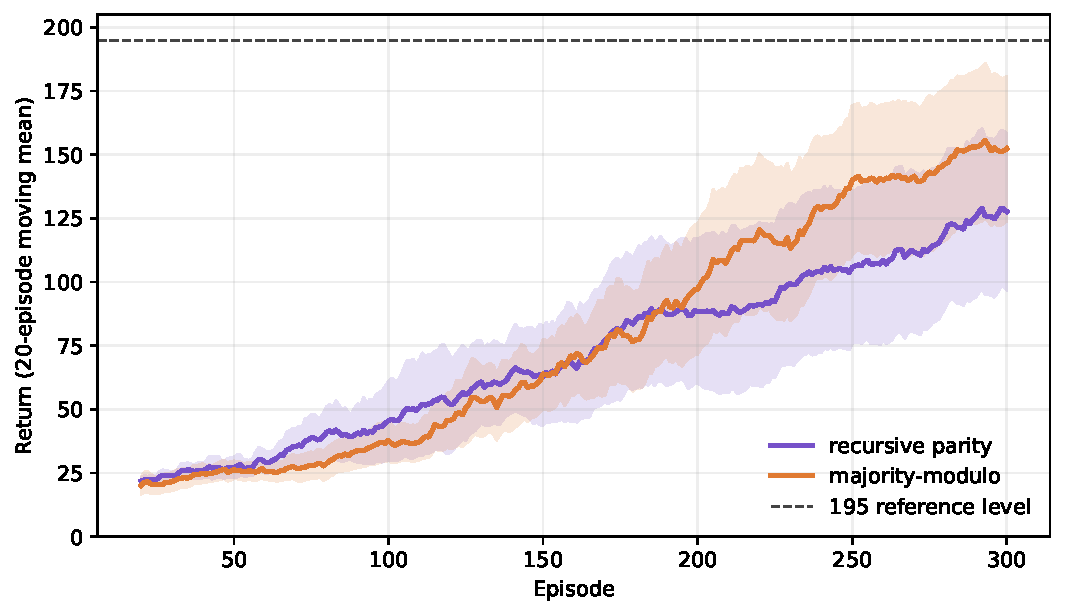
\includegraphics[width=\textwidth]{figures/cartpole_policy_rewards.pdf}
    \caption{CartPole returns.  Curves are 20-episode moving means and shaded
    regions are the standard error over five matched seeds.}
    \label{fig:cartpole-rewards}
  \end{subfigure}\hfill
  \begin{subfigure}[t]{0.39\textwidth}
    \centering
    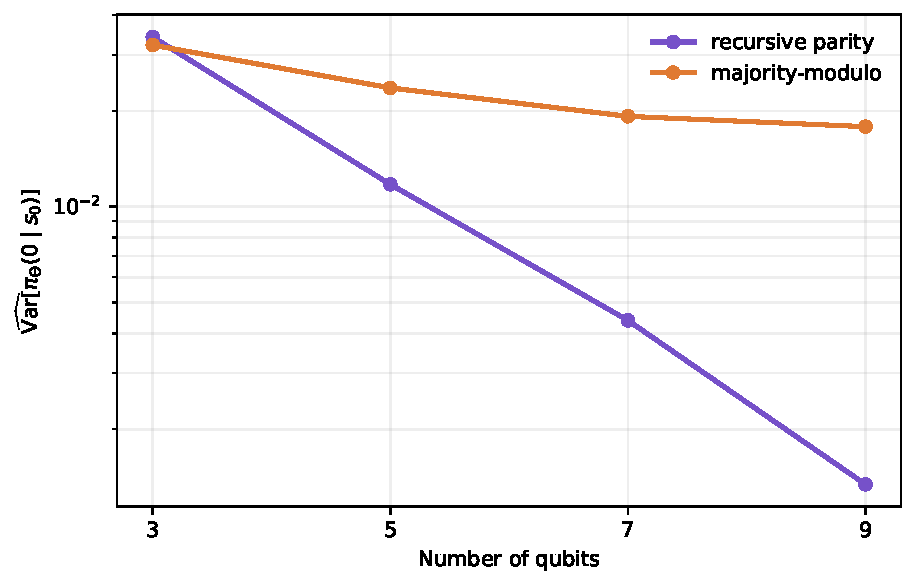
\includegraphics[width=\textwidth]{figures/policy_variance_example.pdf}
    \caption{Initialization variance at fixed $s_0=\bm 0$ and $a=0$, estimated
    from 500 reinitializations at each width.}
    \label{fig:policy-variance-example}
  \end{subfigure}
  \caption{Executable QASP policy examples generated by
  \code{cartpole\_policies\_and\_variance.ipynb}.  Both panels compare exact
  recursive-parity expectation readout with exact majority--modulo sparse
  projectors on one-layer ring graph-IQP circuits.  These finite experiments
  validate the end-to-end workflow; they are not asymptotic performance claims.}
  \label{fig:cartpole-and-variance}
\end{figure*}

The CartPole panel contains $300$ episodes for each of five seeds, with an
imposed $200$-step episode cap.  Over the final 50 episodes, the mean return was
$121.09\pm30.80$ for recursive parity and $147.70\pm28.70$ for
majority--modulo, where the uncertainty is the standard error across seeds.
The overlapping uncertainty bands preclude a ranking claim; the purpose is to
show that both readout contracts participate in the same complete learning
loop.  Every raw episodic return and per-run wall time is stored under
\code{examples/results/}, so alternative smoothing or summary choices do not
require rerunning the quantum simulation.

The second panel demonstrates the public \code{policy\_variance} diagnostic.
For a fixed action $a$ and observation $s_0$, randomized initializations
$\bm\Theta_1,\ldots,\bm\Theta_N$ produce $p_j=\pi_{\bm\Theta_j}(a\mid s_0)$
and the estimator
\begin{equation}
  \widehat{\operatorname{Var}}[\pi_{\bm\Theta}(a\mid s_0)]
  =\frac{1}{N}\sum_{j=1}^{N}(p_j-\bar p)^2,
  \qquad \bar p=\frac{1}{N}\sum_{j=1}^{N}p_j.
  \label{eq:policy-variance-estimator}
\end{equation}
The notebook evaluates the public API separately at each width so the measured
wires and odd majority block remain explicit:
\begin{lstlisting}[caption={Controlled use of 
\code{policy\_variance}.  The notebook's 
\code{variance\_config} returns the complete width-specific dictionary from
\cref{lst:cartpole-policies}.},label={lst:policy-variance}]
for policy_name in ("recursive parity", "majority-modulo"):
    for n_qubits in (3, 5, 7, 9):
        variance, raw_samples = policy_variance(
            policy_class="PQCBorn",
            policy_config_kwargs=variance_config(
                n_qubits, policy_name
            ),
            action=0,
            qubit_list=[n_qubits],
            n_samples=500,
            batch_size=500,
            parallel=False,
            state=torch.zeros(4),
        )
\end{lstlisting}
Fixing \code{action=0} is important: when \code{action=None}, the helper first
samples an action and records the probability of that sampled action, which is
a different random variable.  Likewise, passing
\code{state=torch.zeros(4)} isolates initialization variance at one input;
omitting the state also resamples an observation.  In the plotted one-layer
ring family, the parity estimate decreases from $3.41\times10^{-2}$ at three
qubits to $1.34\times10^{-3}$ at nine, whereas the corresponding majority
estimate changes from $3.22\times10^{-2}$ to $1.78\times10^{-2}$.  This is an
empirical diagnostic for the stated initialization ensemble, not a substitute
for the architecture-specific variance bounds.

\subsubsection{Contextual bandits and AWR}

\code{ContextualBanditTrainer} implements an advantage-weighted regression (AWR) update for one-step tasks \cite{peng2019awr}.  A replay tuple $(s_i,a_i,r_i)$ receives detached weight
\begin{equation}
  w_i=\min\left(w_{\max},
    \exp\left[\frac{r_i-\bar r}{T}\right]\right),
  \qquad
  \mathcal{L}_{\mathrm{AWR}}=-\frac{1}{N}\sum_iw_i\log\pi(a_i\mid s_i),
\end{equation}
where $\bar r$ is an exponential-moving-average baseline.  The trainer evaluates samples one at a time when a quantum layer does not support the requested batch layout, preserving gradients while avoiding a false assumption of vectorized quantum execution.

The companion \code{ContextualBanditEnv} generates bounded continuous contexts
with configurable deterministic, stochastic, raw-dense, or normalized-dense
rewards.  It exposes optimal actions, oracle value, reward bounds, and
serialization.  Its nominal oracle and bounds assume nonnegative reward
scaling, and the normalized oracle omits the step formula's epsilon adjustment;
reported regret should respect those conventions.

\begin{qaspfeature}{\code{ContextualBanditTrainer} and \code{ContextualBanditEnv}}
A matched one-step research workflow: the environment supplies bounded
contexts, configurable rewards, and an oracle, while the trainer applies
advantage-weighted regression to any logits- or probability-valued QASP
policy.  Replay weighting is detached from quantum differentiation.
\end{qaspfeature}

\subsubsection{PPO and TorchRL}

The module-level \code{PPO} utility implements clipped proximal policy optimization with a separate value network and generalized advantage estimation (GAE) \cite{schulman2017ppo}.  With probability ratio $r_t(\bm{\theta})$ and advantage $\widehat A_t$, the actor term is
\begin{equation}
  \mathcal{L}_{\mathrm{clip}}=-\E_t\!\left[
  \min\left(r_t\widehat A_t,
  \operatorname{clip}(r_t,1-\epsilon,1+\epsilon)\widehat A_t\right)
  \right].
\end{equation}
It is combined with value regression, entropy regularization, rollout
minibatches, and gradient clipping.  Each rollout resets its environment, and
both true termination and time-limit truncation mask GAE continuation.  The
maintained \code{TorchRLTrainer} wraps a PQC in a probabilistic categorical
actor and can run manual REINFORCE or a supplied TorchRL loss.  The separate
\code{qasp.rl.trl} collector/PPO code is a historical prototype with known
setup and post-processing limitations, not a second validated PPO route.

\begin{qaspfeature}{\code{PPO} and \code{TorchRLTrainer}}
The maintained module-level \code{PPO} implements clipped updates and GAE
directly; \code{TorchRLTrainer} adapts a quantum module to TensorDict actors
and supplied TorchRL losses.  Compatibility depends on the optional TorchRL
version, and training-return summaries should not be relabelled as independent
evaluation performance.
\end{qaspfeature}

\subsection{Value-based reinforcement learning}
\label{sec:rl-value-based}

Value-based agents learn unconstrained action values and derive behavior from
their ordering, rather than parameterizing a normalized action distribution.
In QASP, the quantum model supplies differentiable Pauli features to a
Q-function, while replay, Bellman targets, exploration, and target-network
updates remain classical.  This separation lets the same trainer compare
\code{PQDQN} models and classical baselines under an identical interaction
and evaluation contract.

\subsubsection{Quantum Q-functions}
\label{sec:pqdqn}

Value-based reinforcement learning requires unconstrained action values rather
than a categorical policy \cite{mnih2015human,hasselt2016deep}.  The
\code{PQDQN} module therefore reuses QASP's
feature maps, ansatzes, devices, and derivative methods, but gives measurement
results a separate Q-function contract.  For Pauli words
$P_1,\ldots,P_J$, define the raw quantum expectations
\begin{equation}
  m_j(s;\bm\theta,\bm\phi)
  =\langle\psi_{\bm\theta,\bm\phi}(s)|P_j|
    \psi_{\bm\theta,\bm\phi}(s)\rangle .
  \label{eq:pqdqn-raw-expectations}
\end{equation}
A readout matrix $C\in\R^{R\times J}$ produces quantum features
\begin{equation}
  \varphi_r(s)=\sum_{j=1}^{J}C_{rj}m_j(s),
  \qquad \bm\varphi(s)=C\bm m(s),
  \label{eq:pqdqn-fixed-readout}
\end{equation}
and the optional affine classical head gives
\begin{equation}
  Q_{\bm\Theta}(s,a)
  =\sum_{r=1}^{R}W_{ar}\varphi_r(s)+b_a,
  \qquad \bm\Theta=(\bm\theta,\bm\phi,W,\bm b).
  \label{eq:pqdqn-q-values}
\end{equation}
There is no softmax or probability clipping: \code{forward} returns one real
action value per action.  Setting \code{fc\_layer=False} returns
$\bm\varphi$ directly and consequently requires $R=A$; because expectation
features are bounded, this direct mode is usually unsuitable for long-horizon
returns.  For flat shared lists and named presets, \code{fc\_bias} defaults to
\code{True}; for nested per-action sums it defaults to \code{False}.  Either
default can be overridden explicitly.

\begin{qaspfeature}{\code{PQDQN}, \code{create\_qfunction}, and \code{draw\_qfunction}}
\code{PQDQN} is an end-to-end differentiable PyTorch action-value model.
Flat Pauli lists expose shared features; nested lists define one unit-weighted
sum per action; and \code{"parity-like"} or
\code{"majority-modulo"} expose the distinct non-identity Pauli-$Z$ terms in
the support of the corresponding decoder-projector decomposition.  Each
supported Pauli expectation reaches the trainable head independently; preset
projector coefficients are not applied.  The model exposes its resolved Pauli
strings and feature matrix, while
\code{draw\_qfunction} exports its executable circuit as Matplotlib or
publication-ready Quantikz.  With \code{device="lightning.pp"} and
\code{diff\_method="backprop"}, the same Q-function uses QASP's differentiable
Pauli engine; gradients reach circuit, input-scaling, and head parameters,
while batches are currently propagated sample by sample.
\end{qaspfeature}

For a flat observable list, $C$ is the identity.  A nested list contains one
nonempty group per action and sums that group's expectations, with leading
minus signs allowed in Pauli specifications.  Named readouts instead compute
the Walsh--Pauli decomposition only to identify its support, remove the
identity, and deduplicate the surviving terms.  In the default
\code{preset\_mode="features"}, $C=I$ on that support: the Q-network does
\emph{not} reconstruct $\langle\Pi_a\rangle$ or an action probability.
Instead, $W$ learns an independent coefficient for every feature and $b_a$
supplies an independent constant offset for every output action.  The
historical reconstruction remains available only through the explicit
compatibility setting \code{preset\_mode="projectors"} with
\code{fc\_bias=False}.  The fast Walsh--Hadamard construction avoids dense
operator matrices; the present guard permits at most 16 measured wires and at
most $2^{22}$ projector-by-basis or feature-matrix entries.

The feature-construction size is selected by \code{preset\_actions}, whereas
\code{n\_actions} always specifies the number of final environment Q-values.
These values may differ.  On four qubits, binary parity
($\code{preset\_actions}=2$) supplies only
$Z_0Z_1Z_2Z_3$.  Four-way parity supplies
\begin{equation}
  \bm z_{\mathrm{par},4}(s)=
  \left(
    \langle Z_0Z_1Z_2Z_3\rangle_s,
    \langle Z_0Z_1Z_2\rangle_s,
    \langle Z_3\rangle_s
  \right),
  \qquad
  \bm Q(s)=W\bm z_{\mathrm{par},4}(s)+\bm b,
  \label{eq:pqdqn-parity-a4}
\end{equation}
where $W\in\R^{2\times3}$ still produces two CartPole actions.  This
four-way preset illustrates the API distinction; it is not one of the four
readouts in the final CartPole comparison.

Majority presets follow the same support-only rule.  For three wires the
signed binary-majority observable has the familiar expansion
\begin{equation}
  M_3=\frac{1}{2}\left(
    Z_0+Z_1+Z_2-Z_0Z_1Z_2
  \right),
  \label{eq:pqdqn-majority-three-wire}
\end{equation}
but the default PQDQN receives the four expectations
$\langle Z_0\rangle$, $\langle Z_1\rangle$, $\langle Z_2\rangle$, and
$\langle Z_0Z_1Z_2\rangle$ separately; it does not apply the displayed
$\pm1/2$ coefficients.  For the study's explicit even block
$\{0,1,2,3\}$, strict majority with ties mapped to zero has support on all 15
non-identity $Z$ products.  The supported four-way construction with blocks
$\{0,1,2\}$ and $\{3\}$ instead yields nine terms:
$Z_0Z_1Z_2Z_3$, $Z_0Z_1Z_2$, $Z_0Z_3$, $Z_1Z_3$, $Z_2Z_3$, and the four
local $Z_i$.  That four-way construction was deliberately excluded from the
final comparison.  Explicit blocks are part of the experiment definition;
automatic balanced odd blocks can leave one measured wire unused.

\begin{table}[t]
\centering
\caption{The four \code{PQDQN} readouts used in the corrected CartPole study.
Named presets use the decomposition support as independent features, not the
decomposition coefficients.  Readout-parameter counts include $W$ and any
bias but exclude circuit and input-scaling parameters.}
\label{tab:pqdqn-readouts}
\small
\begin{tabularx}{\textwidth}{@{}p{0.17\textwidth}p{0.34\textwidth}X p{0.13\textwidth}@{}}
\toprule
Readout & Quantum expectations and feature map & Affine-head contract & Readout parameters \\
\midrule
Shared & $Z_0,Z_1,Z_2,Z_3$ with $C=I_4$ & Four shared features and bias, $\bm Q=W\bm z+\bm b$. & $2\times4+2=10$ \\
Per-action control & $(I+Z_0+Z_2,\ I+Z_1+Z_3)$ & Two fixed sums, followed by a bias-free $2\times2$ head. & $2\times2=4$ \\
Parity $a=2$ & $Z_0Z_1Z_2Z_3$ with $C=I_1$ & One full-register parity feature and two-output bias. & $2\times1+2=4$ \\
Majority $a=2$ & All 15 non-identity four-wire $Z$ products with $C=I_{15}$ & Fifteen independent support features and two-output bias. & $2\times15+2=32$ \\
\bottomrule
\end{tabularx}
\end{table}

\Cref{lst:pqdqn-cartpole} shows the public construction used by the executable
CartPole study.  Batches are broadcast through the compatible angle embedding,
and gradients flow jointly through the circuit angles, trainable input scales,
and the classical head.

\begin{lstlisting}[caption={Constructing and training the four-layer majority-$a=2$
PQDQN, followed by an API-only parity-$a=4$ example with two environment
actions.},label={lst:pqdqn-cartpole}]
from qasp import create_qfunction, draw_qfunction, DeepQLearning

readouts = {
    "shared": {
        "observables": ["Z 0", "Z 1", "Z 2", "Z 3"],
        "fc_bias": True,
    },
    "per_action": {
        "observables": [
            ["I 0", "Z 0", "Z 2"],
            ["I 0", "Z 1", "Z 3"],
        ],
        "fc_bias": False,
    },
    "parity_a2": {
        "observables": "parity-like",
        "preset_actions": 2, "fc_bias": True,
    },
    "majority_a2": {
        "observables": "majority-modulo",
        "preset_actions": 2,
        "majority_blocks": [[0, 1, 2, 3]],
        "fc_bias": True,
    },
}
base = {
    "ansatz": "AngleAnsatz",
    "ansatz_config": {
        "n_layers": 4, "rotations": "YZ",
        "reuploading": True,
        "include_imprimitive": True,
        "imprimitive": "CNOT",
        "imprimitive_pattern": "ring",
        "include_final_imprimitive": True,
    },
    "feature_map": "AngleEmbedding",
    "feature_map_config": {
        "features": 4, "rotations": "Y",
        "input_scaling": True,
    },
    "fc_layer": True,
    "device": "default.qubit",
    "diff_method": "backprop",
    "batch_mode": "broadcast",
}
qfunction = create_qfunction(
    {**base, **readouts["majority_a2"]},
    n_qubits=4, n_actions=2,
)
with DeepQLearning(
    qfunction, env_name="CartPole-v1", seed=7,
    lr=1e-2, gamma=0.99, batch_size=64,
    learning_starts=256, train_frequency=4,
    target_update_interval=100,
    epsilon_decay_steps=8000,
) as agent:
    records = agent.train(num_episodes=400)
    held_out = agent.evaluate(num_episodes=100, seed=30000)

parity_a4 = create_qfunction(
    {**base, "observables": "parity-like",
     "preset_actions": 4, "fc_bias": True},
    n_qubits=4, n_actions=2,
)
assert parity_a4.observable_strings == (
    "ZZZZ 0 1 2 3", "ZZZ 0 1 2", "Z 3",
)
assert parity_a4.fc_layer.in_features == 3
assert parity_a4.fc_layer.out_features == 2

tikz = draw_qfunction(
    qfunction, output="tikz",
    tikz_options={"standalone": True, "compress": True},
)
\end{lstlisting}

\begin{figure*}[p]
\centering
\begin{subfigure}{0.98\textwidth}
  \centering
  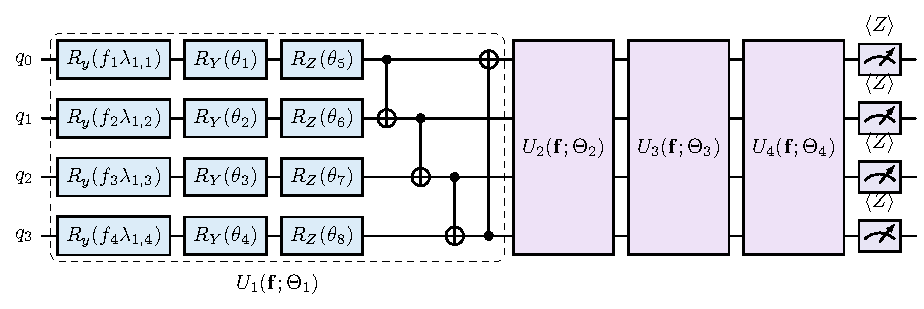
\includegraphics[width=0.90\textwidth]{figures/pqdqn_shared.pdf}
  \caption{Shared four-feature readout with affine bias.  Four input-scaled $R_Y$ encoders,
  trainable $R_Y/R_Z$ rotations, and one CNOT ring are expanded; the remaining
  re-uploading layers are compressed as $U_2,U_3,U_4$.}
\end{subfigure}

\vspace{3mm}
\begin{subfigure}{0.98\textwidth}
  \centering
  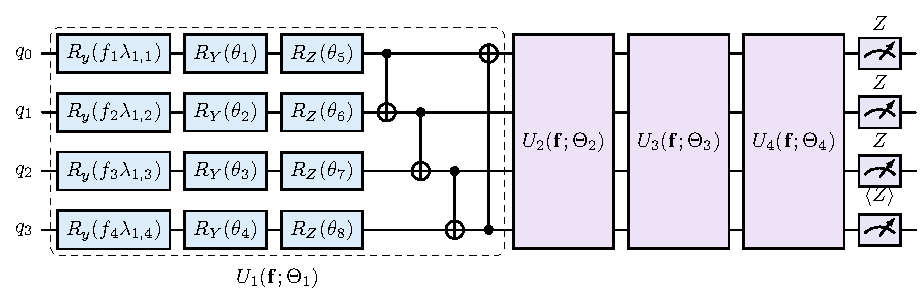
\includegraphics[width=0.90\textwidth]{figures/pqdqn_parity_a4.pdf}
  \caption{Parity $a=4$ feature preset with two output actions.  The exported
  metadata records three independent products:
  $Z_0Z_1Z_2Z_3$, $Z_0Z_1Z_2$, and $Z_3$.  This panel illustrates
  \code{preset\_actions}; the CartPole comparison uses parity $a=2$.}
\end{subfigure}
\caption{Representative \code{PQDQN} circuits exported from the constructed
models with \code{draw\_qfunction(output="tikz")}.  Every study circuit has
four CNOT rings, hence 16 CNOT gates in total.  The per-action and
majority--modulo models have the same gate skeleton.  Measurement meters show
local bases; the Pauli products, trainable affine head, and bias act at the
measurement/classical boundary and are therefore stated in
\cref{tab:pqdqn-readouts}, not drawn as quantum gates.}
\label{fig:pqdqn-circuits}
\end{figure*}

\subsubsection{Deep Q-learning: replay, targets, and exploration}

\code{DeepQLearning} accepts any differentiable module mapping observations to
action values.  A bounded uniform replay buffer stores
$(s_t,a_t,r_t,s_{t+1},d_t)$, where $d_t$ marks true environment termination.
For its default Double-DQN update, the online model selects the next action and
the frozen target model evaluates it:
\begin{align}
  a^*(s')&=\arg\max_b Q_{\bm\Theta}(s',b),\nonumber\\
  y&=r+\gamma(1-d)Q_{\bar{\bm\Theta}}(s',a^*(s')),
  \label{eq:pqdqn-double-target}\\
  \mathcal L_{\mathrm{DQN}}
    &=\frac{1}{B}\sum_{i=1}^{B}
      \operatorname{Huber}\!\left(Q_{\bm\Theta}(s_i,a_i)-y_i\right).
  \label{eq:pqdqn-huber}
\end{align}
Setting \code{double\_dqn=False} replaces the online-network selection in
\cref{eq:pqdqn-double-target} by the maximum target-network value, recovering
the conventional DQN target.  Time-limit truncation and the trainer's
\code{max\_steps} cap end a rollout but do not set $d=1$, so the target
continues to bootstrap; only true environment termination masks the
continuation value.

Exploration is controlled independently of learning.  If $F$ is the cumulative
number of environment frames, QASP uses the clipped linear schedule
\begin{equation}
  \epsilon(F)=\epsilon_{0}+
  \min\!\left(1,\frac{F}{F_{\mathrm{decay}}}\right)
  (\epsilon_{\mathrm{final}}-\epsilon_{0}),
  \label{eq:deepq-epsilon}
\end{equation}
and chooses a uniformly random action with probability $\epsilon(F)$.
Otherwise it evaluates the online Q-function in evaluation mode and takes its
argmax.  This separation makes it possible to change the exploration horizon
without changing the replay warm-up or target-network cadence.

The optimization and data-collection schedules are independently
configurable.  The user can choose \code{optimizer\_class} and
\code{optimizer\_kwargs}, the learning rate, discount, minibatch size, replay
capacity, replay warm-up \code{learning\_starts}, environment-step update
frequency, and the number of gradient steps per update event.  The frozen
target is synchronized every \code{target\_update\_interval} optimizer
updates, rather than environment steps.  Exploration follows a linear
$\epsilon$ schedule controlled by its initial value, final value, and decay
horizon in environment frames.  Huber loss, a configurable gradient-norm cap,
and explicit nonfinite checks protect both classical and differentiable
quantum Q-functions.

The trainer accepts an environment name or a caller-owned Gymnasium instance,
requires zero-based discrete actions, and checks that the Q-function output
width matches the action space.  Observations are optionally passed through a
deterministic \code{observation\_transform}, flattened, and moved to the
Q-function's dtype and device.  A local seeded generator controls exploration
and replay sampling; episode $k$ is reset with \code{seed + k}.  Repeated
\code{train} calls deliberately continue the replay memory, frame count,
update count, episode count, and exploration schedule.  Each returned record
contains the episode return and length, cumulative frames and updates,
current $\epsilon$, and mean minibatch loss.

Three counters make the scheduling semantics explicit.  The frame counter
drives \cref{eq:deepq-epsilon}, \code{learning\_starts}, and
\code{train\_frequency}; the optimizer-update counter drives target-network
synchronization; and the episode counter determines the next reset seed.
Consequently, one update event may perform several optimizer steps through
\code{gradient\_steps}, and target synchronization can occur more often than
the nominal frame frequency might suggest.  An update is attempted only after
the warm-up and on the requested frame cadence, while \code{optimize} also
requires at least \code{batch\_size} stored transitions.  Replay states are
detached CPU clones; a sampled minibatch is moved back to the Q-function's
current dtype and device immediately before evaluation.  This keeps replay
storage backend-independent while preserving gradients through the online
model during the selected-action Huber loss.

Greedy \code{evaluate} runs in a distinct, deterministically seeded
environment and leaves exploration, replay, counters, and the model's
training/evaluation mode unchanged.  When an environment instance is supplied
for training, the caller retains ownership and must provide a separate
evaluation instance; environments created from a name are managed by
\code{close} or the context manager.  Model weights can be checkpointed, but
an exact trainer resume additionally requires optimizer, replay-buffer, and
random-number-generator state, which \code{DeepQLearning} does not save
automatically.  The trainer seed controls its interaction and replay streams;
it does not initialize model weights, so Torch must be seeded before model
construction when matched initializations are required.

\begin{qaspfeature}{\code{DeepQLearning}}
A manual PyTorch DQN trainer for any differentiable module returning one value
per action.  Its main customization groups are:
\begin{itemize}[leftmargin=1.5em,itemsep=1pt,topsep=3pt]
  \item \emph{optimization:} \code{lr}, \code{optimizer\_class},
        \code{optimizer\_kwargs}, \code{gamma}, \code{batch\_size}, and
        \code{max\_grad\_norm};
  \item \emph{replay and updates:} \code{replay\_capacity},
        \code{learning\_starts}, \code{train\_frequency}, and
        \code{gradient\_steps};
  \item \emph{targets and exploration:} \code{double\_dqn},
        \code{target\_update\_interval}, \code{epsilon\_start},
        \code{epsilon\_end}, and \code{epsilon\_decay\_steps};
  \item \emph{interaction:} an environment name or instance,
        \code{max\_steps}, \code{seed}, and a deterministic
        \code{observation\_transform}.
\end{itemize}
Uniform replay, Huber loss, frozen-target updates, nonfinite checks, and
state-preserving greedy evaluation are built in.  Because the trainer is
independent of \code{PQDQN}, the same interaction and evaluation code can be
used for quantum models and classical Q-function baselines.
\end{qaspfeature}

\begin{table}[H]
\centering
\caption{\code{DeepQLearning} customization points.  ``Frame'' means one
environment transition; ``update'' means one optimizer step.  The distinction
is important when \code{train\_frequency} or \code{gradient\_steps} differs
from one.}
\label{tab:deepq-customization}
\small
\begin{tabularx}{\textwidth}{@{}p{0.25\textwidth}p{0.19\textwidth}X@{}}
\toprule
Control & Default & Effect \\
\midrule
\code{qfunction} & required & Any differentiable module with output shape
$({\cdots},|\A|)$; this may be a \code{PQDQN} or a classical baseline. \\
\code{env\_name} & \code{"CartPole-v1"} & Gymnasium identifier or a
caller-owned environment with zero-based discrete actions. \\
\code{lr}, \code{optimizer\_class}, \code{optimizer\_kwargs} &
$10^{-3}$, Adam, \code{None} & Replaces the optimizer without changing the
interaction loop; keyword arguments are forwarded to its constructor. \\
\code{gamma}, \code{batch\_size} & $0.99$, 64 & Discount and uniform replay
minibatch size. \\
\code{replay\_capacity}, \code{learning\_starts} & 10,000, 256 frames & FIFO
memory budget and earliest frame at which updates may begin. \\
\code{train\_frequency}, \code{gradient\_steps} & 1 frame, 1 update & How often
an update event occurs and how many replay updates it performs. \\
\code{double\_dqn}, \code{target\_update\_interval} & \code{True}, 100 updates
& Double-DQN or conventional DQN target and hard-copy cadence. \\
\code{epsilon\_start}, \code{epsilon\_end}, \code{epsilon\_decay\_steps} &
$1.0$, $0.05$, 10,000 frames & Endpoints and duration of the linear
$\epsilon$-greedy schedule. \\
\code{max\_steps}, \code{max\_grad\_norm} & 500, 10 & Episode/evaluation cap
and global gradient-norm clipping threshold. \\
\code{seed}, \code{observation\_transform} & 0, \code{None} & Local
exploration/replay/reset reproducibility and deterministic feature
preprocessing before flattening. \\
\bottomrule
\end{tabularx}
\end{table}

\clearpage
\Cref{lst:deepq-customization} illustrates how the controls compose.  Here a
caller-owned environment is paired with deterministic input compression, an
AdamW optimizer, two replay updates every four frames, vanilla DQN targets,
and a shorter exploration schedule.  The same trainer can instead receive a
quantum \code{PQDQN} with no change to the interaction code.

\begin{lstlisting}[caption={Customizing optimization, replay cadence,
exploration, preprocessing, and environment ownership in
\code{DeepQLearning}.},label={lst:deepq-customization}]
import gymnasium as gym
import numpy as np
import torch
from qasp import DeepQLearning

def compress_cartpole(observation):
    scale = np.array([2.4, 3.0, 0.21, 3.5])
    return np.tanh(np.asarray(observation) / scale)

train_env = gym.make("CartPole-v1")
eval_env = gym.make("CartPole-v1")
agent = DeepQLearning(
    qfunction, train_env,
    optimizer_class=torch.optim.AdamW,
    optimizer_kwargs={"weight_decay": 1e-4},
    lr=3e-3, gamma=0.98,
    batch_size=32, replay_capacity=20_000,
    learning_starts=512,
    train_frequency=4, gradient_steps=2,
    double_dqn=False, target_update_interval=250,
    epsilon_start=0.9, epsilon_end=0.02,
    epsilon_decay_steps=20_000,
    max_steps=500, max_grad_norm=5.0,
    observation_transform=compress_cartpole,
    seed=19,
)
try:
    records = agent.train(num_episodes=300, log_every=25)
    returns = agent.evaluate(
        num_episodes=50, seed=40_000, env=eval_env
    )
finally:
    train_env.close()  # caller owns both environment instances
    eval_env.close()
\end{lstlisting}

The class intentionally keeps the research contract small: replay is uniform,
target transfers are hard copies, the loss is Huber, and the exploration
schedule is linear.  Prioritized replay, $n$-step returns, soft target updates,
reward shaping, callbacks, and full trainer-state serialization are not
constructor options in the current release.  Such changes should therefore be
implemented explicitly rather than inferred from similarly named DQN
frameworks.  Users can nevertheless call \code{select\_action},
\code{optimize}, and \code{sync\_target} directly when building a controlled
outer loop around QASP's tested primitives.

\subsubsection{CartPole value-readout study}
\label{sec:pqdqn-cartpole-results}

The executed notebook
\code{examples/cartpole\_pqdqn\_deep\_q\_learning.ipynb} compares the four
readouts in \cref{tab:pqdqn-readouts}.  Every model uses four qubits, four
$R_Y/R_Z$ ansatz layers, re-uploaded $R_Y$ angle encoding with trainable input
scales, a CNOT ring in every layer including the final layer, and a fully
connected head.  Shared, parity-$a=2$, and majority-$a=2$ use affine bias;
the original identity-containing per-action sums are retained as a bias-free
control.  Consequently the number of trainable readout parameters differs
across configurations as reported in \cref{tab:pqdqn-readouts}.  Training uses analytic \code{default.qubit}
simulation with backpropagation and broadcast batches.  For each readout,
seeds 7--11 receive 400 training episodes with Adam learning rate $10^{-2}$,
$\gamma=0.99$, batch size 64, learning beginning after 256 frames, one update
every four frames, target synchronization every 100 updates, and linear
$\epsilon$ decay over 8000 frames.  Replay capacity is 10,000 and gradients
are clipped to norm 10.

Each trained seed is evaluated greedily on 100 held-out episodes with common
reset seeds 30000--30099.  The five trained seeds---not the resulting 500
evaluation episodes---are the independent experimental units for each
readout.  Moving curves first compute a trailing 20-episode mean within each
seed and then report the across-seed mean and sample standard deviation; the
first 19 episodes are omitted.  Shading is $\pm1$ sample standard deviation,
not a confidence interval, and can extend below zero even though CartPole
returns are positive.  Equal episode budgets yielded unequal environment-step
budgets, ranging from 6,347 to 63,735 frames across the 20 runs.

\begin{figure*}[t]
  \centering
  \begin{subfigure}[t]{0.59\textwidth}
    \centering
    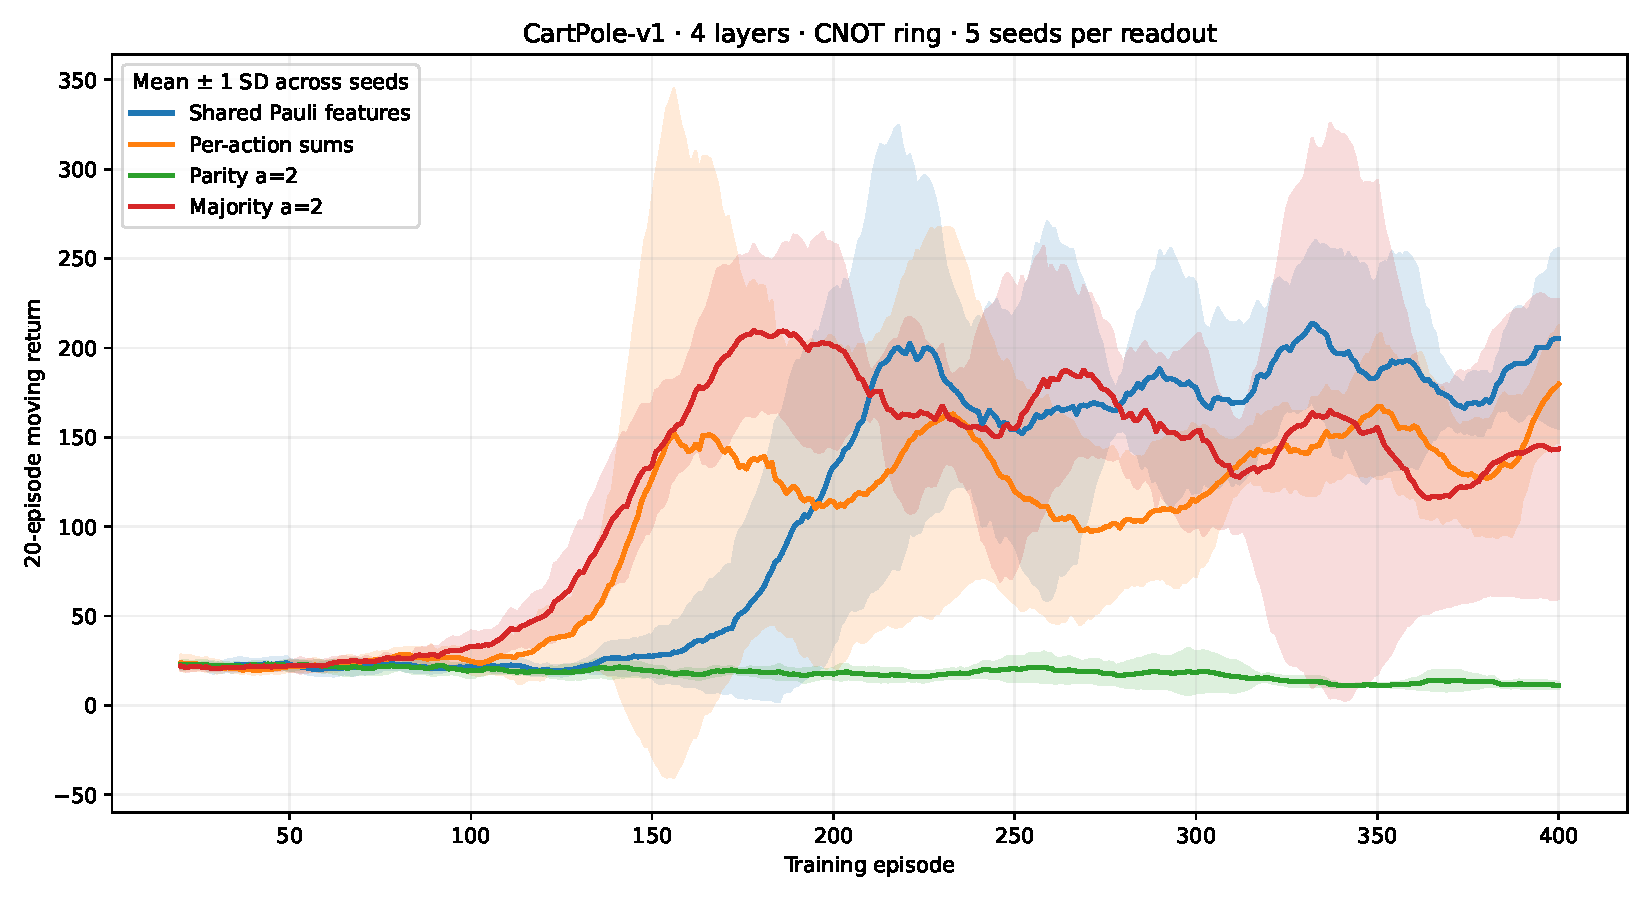
\includegraphics[width=\textwidth]{figures/pqdqn_average_moving_returns.pdf}
    \caption{Mean trailing 20-episode training return; shading is
    $\pm1$ sample SD across the five trained seeds.}
    \label{fig:pqdqn-moving-returns}
  \end{subfigure}\hfill
  \begin{subfigure}[t]{0.39\textwidth}
    \centering
    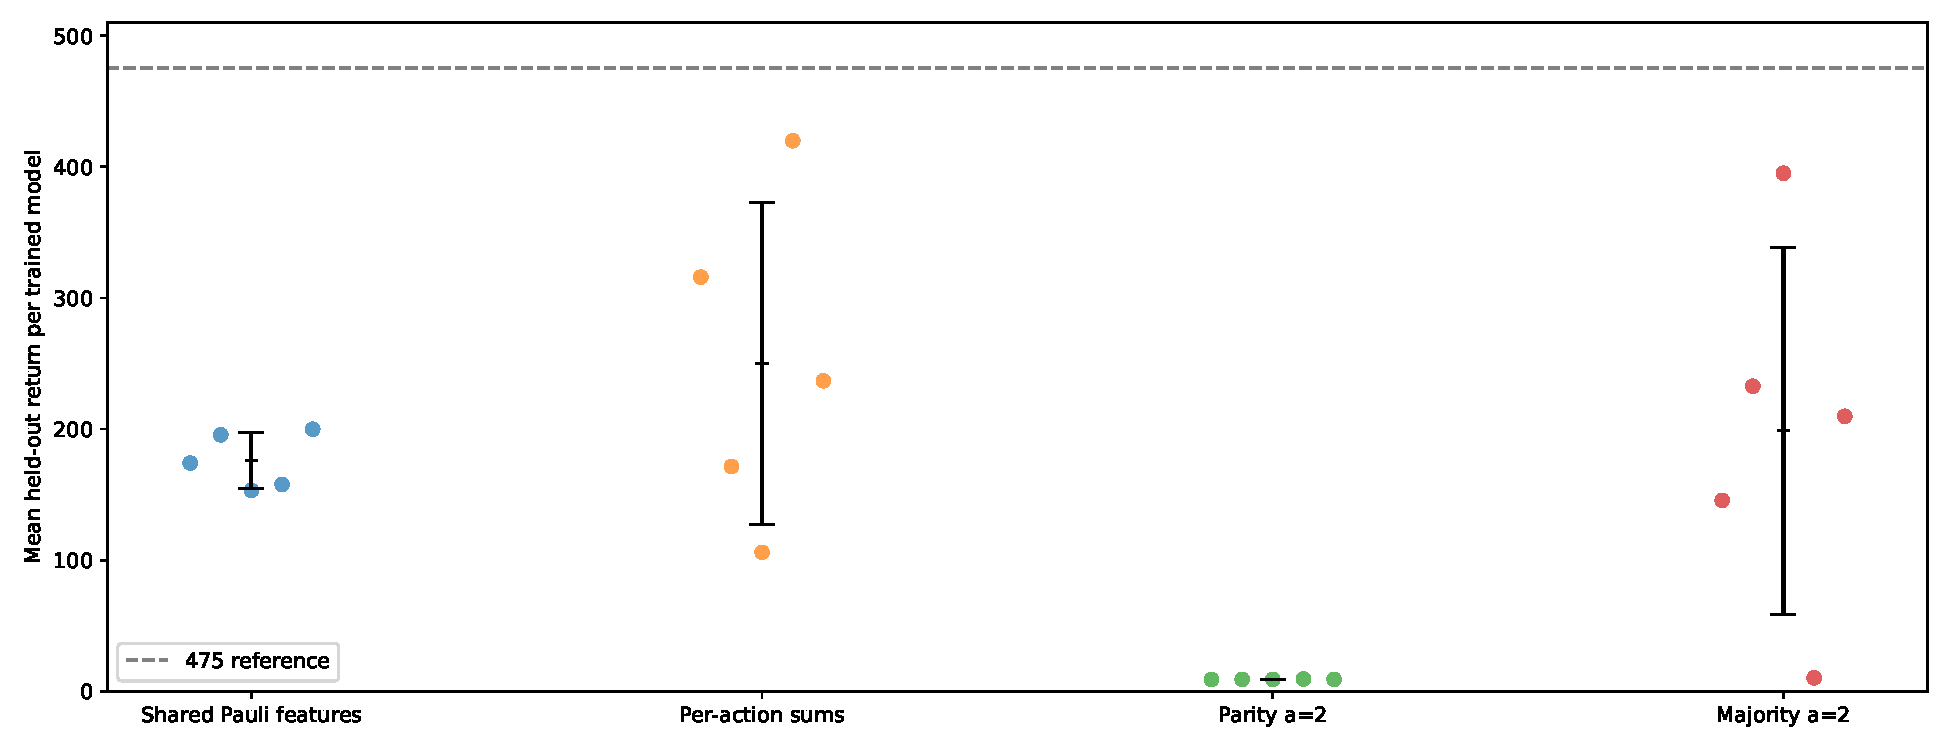
\includegraphics[width=\textwidth]{figures/pqdqn_held_out_returns.pdf}
    \caption{One point per trained seed: mean return over its 100 common-seed
    held-out episodes.  Bars show mean $\pm1$ sample SD across trained seeds.}
    \label{fig:pqdqn-held-out}
  \end{subfigure}
  \caption{Completed PQDQN CartPole comparison.  The horizontal 475 line is a
  reference, not a stopping rule.  All 8,000 training episodes, seed-level
  evaluations, model checkpoints, manifests, and circuit exports are retained
  as machine-readable experiment artifacts.}
  \label{fig:pqdqn-cartpole-results}
\end{figure*}

\begin{table*}[t]
\centering
\caption{PQDQN CartPole outcomes.  Held-out uncertainty is the sample standard
deviation across five independently trained seeds; it is not the standard
error and does not treat evaluation episodes as independent models.}
\label{tab:pqdqn-cartpole-results}
\small
\begin{tabularx}{\textwidth}{@{}p{0.17\textwidth}X p{0.20\textwidth}p{0.16\textwidth}@{}}
\toprule
Readout & Held-out mean for trained seeds 7--11 & Across-seed held-out mean $\pm$ SD & Mean final-20 training return \\
\midrule
Shared Pauli features & 174.12, 195.58, 153.32, 157.80, 199.92 & $176.148\pm21.240$ & 205.28 \\
Per-action sums & 315.89, 171.44, 106.06, 419.78, 236.82 & $249.998\pm122.710$ & 179.64 \\
Parity $a=2$ & 9.19, 9.19, 9.19, 9.49, 9.19 & $9.250\pm0.134$ & 11.08 \\
Majority $a=2$ & 145.63, 232.69, 395.11, 10.36, 209.77 & $198.712\pm139.770$ & 143.43 \\
\bottomrule
\end{tabularx}
\end{table*}

Under this configuration and budget, per-action sums have the highest observed
mean held-out return.  Shared local-$Z$ features have a lower observed mean but
substantially smaller between-seed variation.  The 15-feature majority model
learns useful control for several seeds but fails on one, whereas the
single-feature parity model does not learn useful control.  No trained model's
held-out mean reaches 475.  These comparisons jointly change feature content,
bias, and the number of trainable readout parameters; in particular, the
corrected majority result is not a bias-only ablation against the historical
projector-reconstruction experiment.  With only five independently trained
seeds per readout and no classical function-approximation baseline, the data do
not establish reliable solution of CartPole, statistically demonstrated
superiority, general readout rankings, or quantum advantage.


\addtocontents{toc}{\protect\setcounter{tocdepth}{2}}
\section{Quantum kernels}
\label{sec:kernels}

The kernel layer now exposes a complete high-level path from a QASP feature
map to a train, validation, or test Gram matrix.  It reuses the same circuit
templates, builder, device selection, differentiation methods, and PyTorch
connection as the other task modules.  Given an
encoding circuit
\begin{equation}
  \lvert\psi_{\bm{\theta}}(\bm{x})\rangle
  =U_{\bm{\theta}}(\bm{x})\lvert0\rangle^{\otimes n},
  \label{eq:kernel-feature-state}
\end{equation}
a kernel is evaluated pairwise to form
\begin{equation}
  [K_{XY}]_{ij}=k_{\bm{\theta}}(\bm{x}_i,\bm{y}_j),
  \qquad
  K_{XX}\in\R^{N\times N}.
  \label{eq:kernel-gram}
\end{equation}
This is the quantum-feature-space construction used by kernel methods
\cite{schuld2019feature,havlicek2019supervised}.  In QASP, the resulting array
can be passed directly to a precomputed-kernel estimator; when the circuit is
trainable, the same Gram computation can instead remain inside a PyTorch
computation graph.

\begin{figure}[H]
\centering
\resizebox{0.98\textwidth}{!}{%
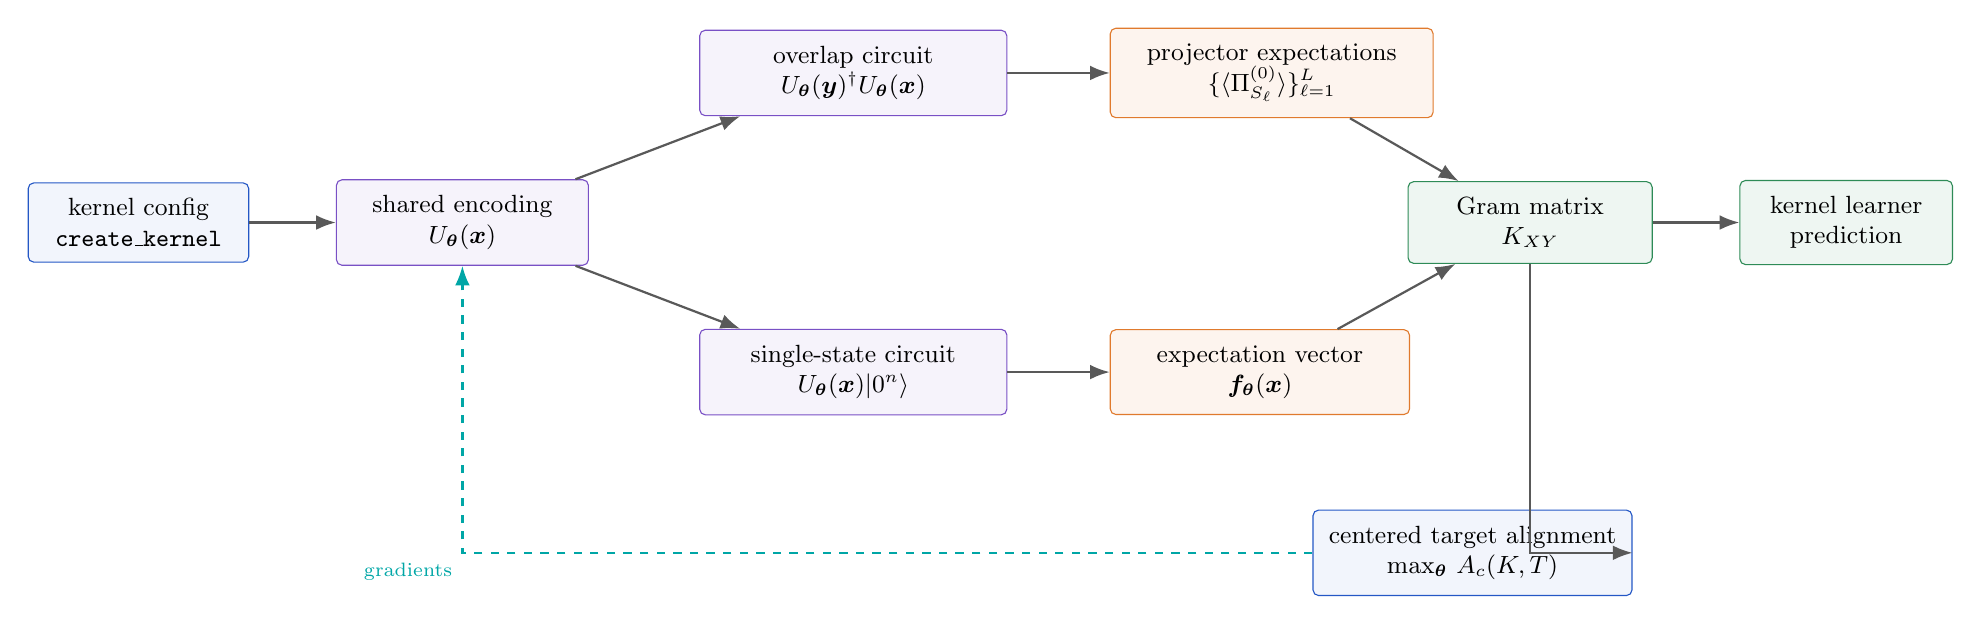
\begin{tikzpicture}[
  box/.style={draw,rounded corners=2pt,align=center,minimum height=10mm,inner sep=2mm,font=\small},
  config/.style={box,draw=qaspblue,fill=qaspblue!6},
  circuit/.style={box,draw=qasppurple,fill=qasppurple!7},
  measure/.style={box,draw=qasporange,fill=qasporange!8},
  result/.style={box,draw=qaspgreen,fill=qaspgreen!8},
  flow/.style={-{Latex[length=2.5mm]},thick,draw=black!65},
  feedback/.style={-{Latex[length=2.5mm]},thick,dashed,draw=qaspcyan},
  node distance=9mm and 11mm
]
\node[config,minimum width=28mm] (cfg) {kernel config\\\code{create\_kernel}};
\node[circuit,right=of cfg,minimum width=32mm] (encoding) {shared encoding\\$U_{\bm\theta}(\bm{x})$};
\node[circuit,above right=8mm and 14mm of encoding,minimum width=39mm] (overlap) {overlap circuit\\$U_{\bm\theta}(\bm{y})^\dagger U_{\bm\theta}(\bm{x})$};
\node[circuit,below right=8mm and 14mm of encoding,minimum width=39mm] (single) {single-state circuit\\$U_{\bm\theta}(\bm{x})\lvert0^n\rangle$};
\node[measure,right=13mm of overlap,minimum width=41mm] (overlapread) {projector expectations\\$\{\langle\Pi_{S_\ell}^{(0)}\rangle\}_{\ell=1}^{L}$};
\node[measure,right=13mm of single,minimum width=38mm] (features) {expectation vector\\$\bm f_{\bm\theta}(\bm{x})$};
\node[result,right=18mm of $(overlapread)!0.5!(features)$,minimum width=31mm] (gram) {Gram matrix\\$K_{XY}$};
\node[result,right=of gram,minimum width=27mm] (learner) {kernel learner\\prediction};
\node[config,below=12mm of features,xshift=27mm,minimum width=35mm] (kta) {centered target alignment\\$\max_{\bm\theta}\,A_c(K,T)$};

\draw[flow] (cfg) -- (encoding);
\draw[flow] (encoding) -- (overlap);
\draw[flow] (encoding) -- (single);
\draw[flow] (overlap) -- (overlapread);
\draw[flow] (single) -- (features);
\draw[flow] (overlapread) -- (gram);
\draw[flow] (features) -- (gram);
\draw[flow] (gram) -- (learner);
\draw[flow] (gram.south) |- (kta.east);
\draw[feedback] (kta.west) -| node[below left,font=\scriptsize,text=qaspcyan]{gradients} (encoding.south);
\end{tikzpicture}}
\caption{The QASP quantum-kernel stack.  One resolved encoding circuit feeds
either the projector-configurable \code{FidelityKernel} or single-state
expectation features for \code{ProjectedKernel}.  The pairwise result is
assembled into a Gram matrix for a classical kernel learner.  For trainable
encodings, centered kernel--target alignment differentiates through the same
Gram computation and updates the circuit parameters.}
\label{fig:kernel-stack}
\end{figure}

\subsection{Shared construction and factory contract}
\label{sec:kernel-factory}

The kernel factory mirrors \code{create\_model}.  A parameter-free kernel
applies the selected \code{AngleEmbedding} or \code{NeuralEmbedding} feature
map \code{reps} times.  Supplying \code{ansatz} and
\code{ansatz\_config} instead constructs a trainable
$U_{\bm\theta}(\bm{x})$ from \code{IQPAnsatz} or \code{AngleAnsatz}; the same
$\bm\theta$ is shared by both sides of every pairwise circuit.  Device,
differentiation method, shots, and MPI selection are forwarded to
\code{CircuitBuilder}, so kernels follow the same execution contract as QASP
models.  Inputs are checked to be finite arrays of shape
$(N,d)$, and a cross Gram matrix accepts independent $X$ and $Y$ collections.
\code{gram(..., return\_tensor=True)} preserves the graph for trainable quantum
weights, whereas NumPy-returning convenience paths detach it.  These input
conversion paths do not promise derivatives with respect to user-supplied
input arrays.

\begin{qaspfeature}{\code{create\_kernel}}
\code{create\_kernel(config, n\_qubits)} resolves one of two continuous-input
classes: \code{FidelityKernel} or \code{ProjectedKernel}.  Global and
localized fidelity are configurations of the same class, selected only by the
optional \code{projectors} list.  Nontrainable feature maps use a fixed
encoding; adding an ansatz creates a PyTorch-backed trainable kernel whose
\code{parameters()} can be optimized.
\end{qaspfeature}

\begin{qaspfeature}{\code{draw\_kernel}}
\code{draw\_kernel} accepts either a resolved kernel or a configuration and
traces the circuit that is actually evaluated.  Fidelity kernels show the
two-input overlap circuit, whereas a projected kernel shows its single-state
expectation circuit.  Setting \code{output="tikz"} returns editable Quantikz;
\code{tikz\_options} controls standalone output, symbolic parameters, wire
labels, gate colors, and repeated-layer compression.
\end{qaspfeature}

\begin{lstlisting}[caption={Constructing, evaluating, and drawing a global-fidelity kernel through the public factory.},label={lst:kernel-factory}]
import numpy as np
from qasp import create_kernel, draw_kernel

X_train = np.array([[0.10, 0.20, 0.15], [0.20, 0.10, 0.12],
                    [0.90, 1.10, 1.00], [1.00, 0.80, 0.92]])
X_test = np.array([[0.15, 0.25, 0.18],
                   [0.95, 0.85, 0.90]])

config = {
    "kernel_type": "fidelity",
    "feature_map": "AngleEmbedding",
    "feature_map_config": {
        "rotations": "Y", "imprimitive_pattern": "ring"
    },
    "reps": 2,
    "device": "default.qubit",
}
kernel = create_kernel(config, n_qubits=3)
K_train = kernel.gram(X_train)          # shape (4, 4)
K_test = kernel.gram(X_test, X_train)   # shape (2, 4)
tikz = draw_kernel(
    kernel, x=X_train[0], y=X_train[1], output="tikz",
    tikz_options={"standalone": True,
                  "symbolic_parameters": True},
)
\end{lstlisting}

\subsection{One projector-configurable fidelity kernel}
\label{sec:fidelity-kernel}

Global and localized overlap similarities are now two configurations of the
same \code{FidelityKernel}, rather than separate classes.  Define the overlap
state
\begin{equation}
  \lvert\varphi_{\bm\theta}(\bm{x},\bm{y})\rangle
  =U_{\bm\theta}(\bm{y})^\dagger
   U_{\bm\theta}(\bm{x})\lvert0^n\rangle.
  \label{eq:kernel-overlap-state}
\end{equation}
For a nonempty wire subset $S\subseteq[n]$, QASP's label
\code{"P i j ..."} represents the zero-state subsystem projector
\begin{align}
  \Pi_S^{(0)}
  &:=\left(\bigotimes_{i\in S}\lvert0\rangle\langle0\rvert_i\right)
     \otimes I_{\bar S} \notag\\
  &=2^{-|S|}\prod_{i\in S}(I+Z_i)
   =2^{-|S|}\sum_{T\subseteq S}Z_T,
  \qquad Z_T:=\prod_{i\in T}Z_i,
  \label{eq:fidelity-projector-expansion}
\end{align}
with $Z_\varnothing=I$.  If the configuration contains
$\mathcal P=(S_1,\ldots,S_L)$, the implemented similarity is the arithmetic
mean of the selected projector probabilities,
\begin{equation}
  k_{\mathcal P}(\bm{x},\bm{y})
  =\frac{1}{L}\sum_{\ell=1}^{L}
    \langle\varphi_{\bm\theta}(\bm{x},\bm{y})\rvert
    \Pi_{S_\ell}^{(0)}
    \lvert\varphi_{\bm\theta}(\bm{x},\bm{y})\rangle.
  \label{eq:projector-fidelity-kernel}
\end{equation}
Omitting \code{projectors} creates the single default label containing every
wire, $\mathcal P=([n])$.  Equation~\eqref{eq:projector-fidelity-kernel} then
reduces to the global fidelity
\begin{equation}
  k_{[n]}(\bm{x},\bm{y})
  =\left|\langle0^n\rvert U_{\bm\theta}(\bm{y})^\dagger
    U_{\bm\theta}(\bm{x})\lvert0^n\rangle\right|^2
  =\left|\langle\psi_{\bm\theta}(\bm{y})
    \mid\psi_{\bm\theta}(\bm{x})\rangle\right|^2.
  \label{eq:global-fidelity-kernel}
\end{equation}
Thus the default exact train Gram matrix is positive semidefinite.  Proper
subsets localize the comparison, while lists may mix different locality
scales.  Every configuration satisfies $0\leq k_{\mathcal P}\leq1$ and
$k_{\mathcal P}(\bm{x},\bm{x})=1$; an average involving proper subsets is not,
in general, guaranteed to be positive semidefinite.  QASP symmetrizes a train
Gram matrix but leaves its spectrum visible to the user.

For example, on three qubits
\code{projectors=["P 0 1", "P 0 1 2"]} gives
\begin{equation}
  k_{\mathcal P}(\bm{x},\bm{y})
  =\frac{1}{2}\left(
    \langle\Pi_{\{0,1\}}^{(0)}\rangle_{\varphi}
   +\langle\Pi_{\{0,1,2\}}^{(0)}\rangle_{\varphi}\right),
  \label{eq:mixed-projector-fidelity-example}
\end{equation}
where the exact Pauli decompositions are
\begin{align}
  \Pi_{\{0,1\}}^{(0)}
  &=\tfrac14(I+Z_0+Z_1+Z_0Z_1), \notag\\
  \Pi_{\{0,1,2\}}^{(0)}
  &=\tfrac18(I+Z_0+Z_1+Z_2+Z_0Z_1+Z_0Z_2+Z_1Z_2+Z_0Z_1Z_2).
  \label{eq:mixed-projector-pauli-expansion}
\end{align}
The first term probes a two-qubit subsystem and the second is the global
three-qubit fidelity.  This is an exact projector average, not the earlier
interface based on a manually supplied list of $Z$ observables.

\begin{qaspfeature}{\code{FidelityKernel(projectors=...)}}
The unified overlap-fidelity class.  With no \code{projectors} argument it
measures the global all-zero projector.  Each label \code{"P i j ..."}
selects the joint all-zero projector on those wires and the identity
elsewhere; multiple entries are averaged.  The object exposes normalized or
unnormalized train/cross Gram matrices, differentiable tensor output,
\code{projector\_labels}, \code{projector\_wires}, and Quantikz drawing.
The removed \code{"local"} and \code{"local\_fidelity"} factory names now
fail explicitly, preventing silent use of the superseded class contract.
\end{qaspfeature}

\begin{lstlisting}[caption={The same \code{FidelityKernel} class in global and mixed-locality projector configurations.},label={lst:projector-fidelity}]
global_kernel = create_kernel({
    **config, "kernel_type": "fidelity",
}, n_qubits=3)

localized_kernel = create_kernel({
    **config, "kernel_type": "fidelity",
    "projectors": ["P 0 1", "P 0 1 2"],
}, n_qubits=3)

K_global = global_kernel.gram(X_train)
K_localized = localized_kernel.gram(X_train)
assert localized_kernel.projector_wires == [[0, 1], [0, 1, 2]]
\end{lstlisting}

\subsection{Projected expectation-feature kernel}
\label{sec:projected-kernel}

The projected kernel replaces a global state overlap by a vector of measured
features \cite{huang2021power}.  For observables
$\mathcal O=\{O_1,\ldots,O_m\}$, QASP evaluates
\begin{equation}
  f_\ell(\bm{x})
  =\langle0^n\rvert U_{\bm\theta}(\bm{x})^\dagger O_\ell
    U_{\bm\theta}(\bm{x})\lvert0^n\rangle,
  \qquad
  \bm f_{\bm\theta}(\bm{x})=(f_1,\ldots,f_m),
  \label{eq:projected-quantum-features}
\end{equation}
followed by a weighted Gaussian kernel in this measured feature space,
\begin{equation}
  k_{\mathrm P}(\bm{x},\bm{y})
  =\exp\!\left[-\gamma\sum_{\ell=1}^{m}w_\ell
    \bigl(f_\ell(\bm{x})-f_\ell(\bm{y})\bigr)^2\right],
  \quad \gamma\geq0,\quad w_\ell\geq0.
  \label{eq:projected-kernel}
\end{equation}
The defaults are all one-qubit $X_i$, $Y_i$, and $Z_i$ expectations with
unit weights.  Nonnegative weights make
\cref{eq:projected-kernel} a classical Gaussian kernel on an explicitly
computed quantum feature vector, hence it is positive semidefinite and has a
unit diagonal.  The \code{features(X)} method exposes this intermediate
representation for analysis or reuse.

\begin{qaspfeature}{\code{ProjectedKernel}}
A weighted radial-basis kernel over quantum expectation features.  Users may
select arbitrary valid Pauli strings, inspect the feature matrix, and control
the bandwidth $\gamma$ and nonnegative feature weights.  The circuit is
evaluated once per input feature vector rather than once for every input pair.
\end{qaspfeature}

\begin{figure*}[p]
\centering
\begin{subfigure}{0.98\textwidth}
  \centering
  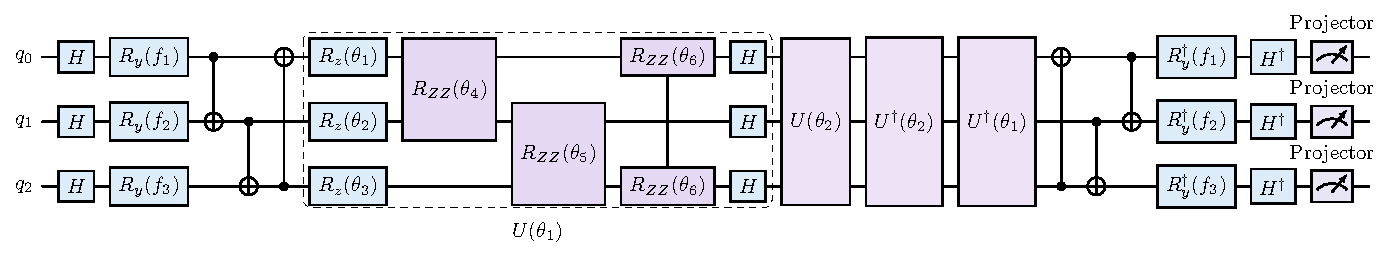
\includegraphics[width=\textwidth]{figures/kernel_fidelity_global.pdf}
  \caption{Default \code{FidelityKernel}: the compressed IQP encoding
  $U_{\bm\theta}(\bm{x})$ is followed by
  $U_{\bm\theta}(\bm{y})^\dagger$ and the all-qubit zero projector.}
  \label{fig:kernel-global-circuit}
\end{subfigure}

\vspace{4mm}
\begin{subfigure}{0.98\textwidth}
  \centering
  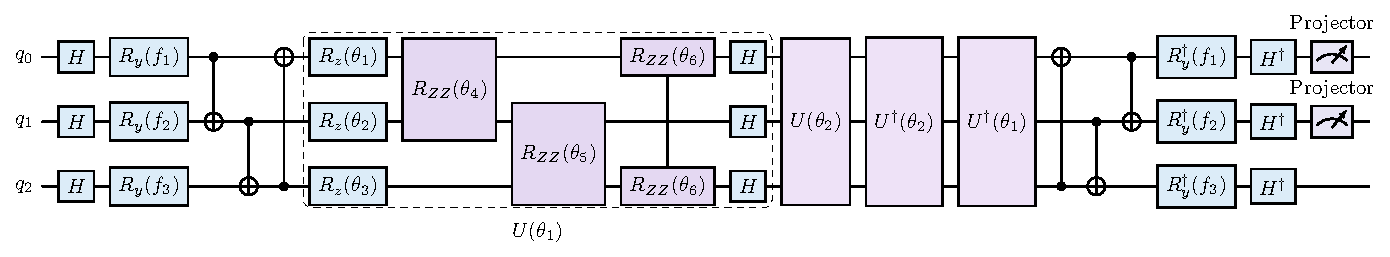
\includegraphics[width=\textwidth]{figures/kernel_fidelity_localized.pdf}
  \caption{The same class with \code{projectors=["P 0 1"]}: only wires
  $0$ and $1$ enter the zero-state projector, while wire $2$ remains
  unmeasured.}
  \label{fig:kernel-localized-circuit}
\end{subfigure}

\vspace{4mm}
\begin{subfigure}{0.86\textwidth}
  \centering
  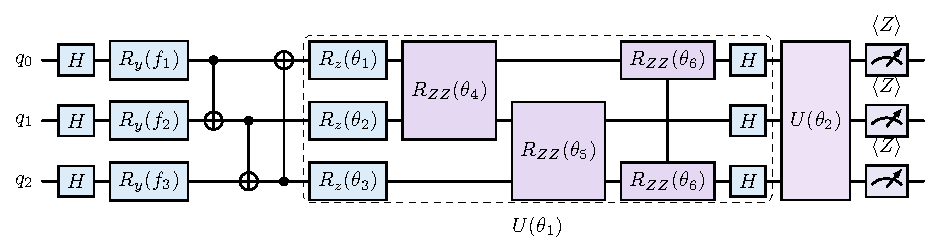
\includegraphics[width=\textwidth]{figures/kernel_projected.pdf}
  \caption{\code{ProjectedKernel}: a single encoding circuit yields local
  expectation features, here $\langle Z_0\rangle$, $\langle Z_1\rangle$, and
  $\langle Z_2\rangle$, before classical weighted-Gaussian post-processing.}
  \label{fig:kernel-projected-circuit}
\end{subfigure}

\caption{Quantum-kernel circuits traced from executable kernel objects using
\qasp{}'s \code{draw\_kernel(output="tikz")} path.  The accompanying
\code{render\_kernel\_circuits.py} script retains the editable standalone
Quantikz source and compiles these vector PDFs plus PNG previews.  Symbolic
parameters, semantic colors, inverse-layer order, and compression are supplied
by QASP rather than reconstructed for the manuscript.}
\label{fig:kernel-circuit-gallery}
\end{figure*}

\subsection{Trainable kernels and centered target alignment}
\label{sec:kta}

Adding an ansatz makes each preceding kernel depend on shared variational
parameters $\bm\theta$.  When the Gram matrix is requested as a tensor, QASP
preserves its autodifferentiation graph.  The package trains these
parameters by centered kernel--target alignment
\cite{cortes2012alignment}.  For labels $y_1,\ldots,y_N$, define
\begin{equation}
  T_{ij}=\mathbf{1}\{y_i=y_j\},
  \qquad
  H=I_N-\frac{1}{N}\bm{1}\bm{1}^{\mathsf T},
  \qquad K_c=HKH,\quad T_c=HTH,
  \label{eq:kta-centering}
\end{equation}
and
\begin{equation}
  A_c(K,T)
  =\frac{\langle K_c,T_c\rangle_{\mathrm F}}
  {\lVert K_c\rVert_{\mathrm F}\lVert T_c\rVert_{\mathrm F}}.
  \label{eq:centered-kta}
\end{equation}
The binary or multiclass target matrix rewards large within-class similarity
relative to between-class similarity.  \code{KernelTargetAlignment} minimizes
$-A_c$ with Adam by default, accepts a user optimizer, and can estimate each
update from a seeded random minibatch to reduce the quadratic Gram cost.

\begin{qaspfeature}{\code{KernelTargetAlignment} and \code{align\_kernel}}
\code{KernelTargetAlignment.fit} differentiates centered alignment through a
trainable kernel and returns loss and alignment histories.  The convenience
function \code{align\_kernel} performs the same fit and returns the optimized
kernel together with its history.  A parameter-free kernel fails explicitly
instead of silently performing a no-op optimization.
\end{qaspfeature}

\begin{lstlisting}[caption={A trainable IQP fidelity kernel and centered target-alignment update.},label={lst:kta-kernel}]
import torch
from qasp import (KernelTargetAlignment, create_kernel,
                  target_alignment)

y_train = np.array([0, 0, 1, 1])
trainable_config = {
    "kernel_type": "fidelity",
    "feature_map": "AngleEmbedding",
    "feature_map_config": {
        "rotations": "Y", "imprimitive_pattern": "ring"
    },
    "ansatz": "IQPAnsatz",
    "ansatz_config": {
        "n_layers": 2, "imprimitive_pattern": "ring",
        "reuploading": True,
    },
    "init": "small_normal",
    "device": "default.qubit",
}
torch.manual_seed(3)
kernel = create_kernel(trainable_config, n_qubits=3)
before = target_alignment(kernel.gram(X_train), y_train)
history = KernelTargetAlignment(kernel).fit(
    X_train, y_train, steps=5, lr=0.02, seed=3, verbose=False
)
after = target_alignment(kernel.gram(X_train), y_train)
\end{lstlisting}

\subsection{Fisher-information kernel}
\label{sec:fisher-kernel}

\code{QFKernel} remains a separate, distribution-geometric construction for
bit-string inputs.  Given a probability-valued QNode $q_{\bm\theta}(z)$, it
precomputes the score for each computational-basis string,
\begin{equation}
  \bm{s}_{\bm{\theta}}(z)
  =\nabla_{\bm{\theta}}\log q_{\bm{\theta}}(z)
  =\frac{\nabla_{\bm{\theta}}q_{\bm{\theta}}(z)}{q_{\bm{\theta}}(z)},
  \label{eq:qf-score}
\end{equation}
and constructs
\begin{equation}
  k_{\mathrm{QF}}(z,z')
  =\bm{s}_{\bm{\theta}}(z)^{\mathsf T}
  \left(F+\lambda I\right)^{-1}
  \bm{s}_{\bm{\theta}}(z').
  \label{eq:fisherkernel}
\end{equation}
The metric $F$ can be PennyLane's quantum or classical Fisher matrix.  QASP
solves the regularized system rather than explicitly forming its inverse.
Unlike the continuous-input feature kernels above, the current implementation
enumerates every basis string and precomputes its score; its memory and circuit
cost are therefore exponential in the number of qubits.  Zero model
probabilities can make the score division singular, and the legacy
\code{normalize} option is currently unused.  It is intended for small-system
geometry experiments, including investigations motivated by
vanishing-similarity concerns \cite{suzuki2024qfk}.

\begin{qaspfeature}{\code{QFKernel}}
A regularized Fisher-score kernel for bit-string data.  It reuses a trained
probability-valued QNode, constructs quantum or classical Fisher geometry,
solves the metric system, and returns a Gram matrix.  Its exhaustive basis
score table, zero-probability sensitivity, and unused legacy normalization
flag make the present API a small-system research tool rather than a drop-in
large-width kernel.
\end{qaspfeature}

\Needspace{8\baselineskip}
\begin{lstlisting}[caption={Constructing a Fisher-information kernel from a trained probability-valued QNode and its parameters.},label={lst:qfkernel}]
from qasp import QFKernel

qf_kernel = QFKernel(qnode, params, fisher="quantum",
                     lambda_reg=1e-2)
gram_matrix = qf_kernel(data)
\end{lstlisting}

\subsection{Executable IQP example and validation}
\label{sec:kernel-example}

The release includes \code{examples/iqp\_quantum\_kernels.py} and an
accompanying validation notebook.  The script builds the two continuous-input
kernel classes from a common three-qubit IQP configuration.  It evaluates the
default global fidelity, the same \code{FidelityKernel} with user-defined
projector subsets, and a projected kernel using all single-qubit $X$, $Y$, and
$Z$ expectations:

\begin{lstlisting}[caption={Switching the fidelity projector list and the projected-kernel readout without changing the shared IQP circuit configuration.},label={lst:kernel-families}]
base = {
    "feature_map": "AngleEmbedding",
    "feature_map_config": {
        "rotations": "Y", "imprimitive_pattern": "ring"
    },
    "ansatz": "IQPAnsatz",
    "ansatz_config": {
        "n_layers": 2, "imprimitive_pattern": "ring",
        "reuploading": True,
    },
    "init": "zeros", "device": "default.qubit",
}

localized = create_kernel({
    **base, "kernel_type": "fidelity",
    "projectors": ["P 0 1", "P 0 2", "P 0 1 2"],
}, n_qubits=3)

projected = create_kernel({
    **base, "kernel_type": "projected",
    "observables": ["X 0", "Y 0", "Z 0",
                    "X 1", "Y 1", "Z 1",
                    "X 2", "Y 2", "Z 2"],
    "gamma": 0.5,
}, n_qubits=3)

K_localized = localized.gram(X_train)
K_projected = projected.gram(X_train)
\end{lstlisting}

For the committed example and its fixed data, the global-fidelity test-versus-
train matrix has shape $2\times4$, and an explicit all-qubit projector
\code{"P 0 1 2"} agrees with the default global fidelity to machine precision
in the displayed run.  The localized projector list is parsed as
$[\{0,1\},\{0,2\},\{0,1,2\}]$.  The displayed trainable run changes centered
alignment from $0.9972$ to $0.9973$ over five deliberately short steps; it
is a gradient-path smoke test, not a learning-performance claim.  The focused
kernel and Quantikz-export modules contain 39 passing tests covering factory
construction, removal of the former local-fidelity aliases, projector parsing
and averaging, train/cross Gram conventions, unit diagonals, symmetry,
positive semidefiniteness where guaranteed, differentiability, parameter
updates, invalid configurations, gate scheduling, measurement notation,
symbolic labels, colors, standalone output, and repeated-layer compression.
The notebook additionally demonstrates precomputed-kernel classifiers and
circuit drawings.  These examples validate software contracts on small
simulators; they do not establish quantum advantage or generalization
superiority.

\section{Parameterized quantum classifiers}
\label{sec:classifiers}

The classifier layer turns the shared QASP circuit construction into a
supervised model for binary or multiclass labels, following the parameterized
quantum-classifier setting exemplified by data re-uploading models
\cite{perezsalinas2020data}.  It deliberately separates
the quantum measurement contract from the classical meaning assigned to its
outputs.  A probability-readout classifier aggregates Born probabilities into
genuine class probabilities, whereas an expectation-readout classifier uses
observable values as signed or multiclass scores.  This distinction determines
which predictions, calibration map, and loss functions are mathematically
appropriate.

\begin{figure}[H]
\centering
\resizebox{0.98\textwidth}{!}{%
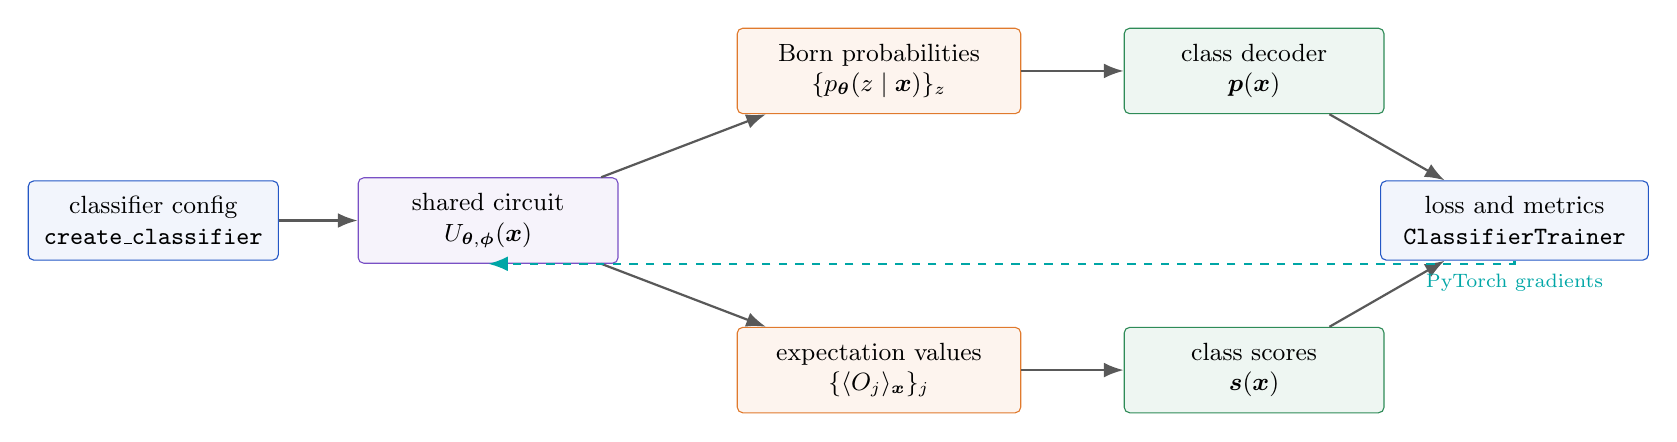
\begin{tikzpicture}[
  box/.style={draw,rounded corners=2pt,align=center,minimum height=10mm,inner sep=2mm,font=\small},
  config/.style={box,draw=qaspblue,fill=qaspblue!6},
  circuit/.style={box,draw=qasppurple,fill=qasppurple!7},
  measure/.style={box,draw=qasporange,fill=qasporange!8},
  result/.style={box,draw=qaspgreen,fill=qaspgreen!8},
  flow/.style={-{Latex[length=2.5mm]},thick,draw=black!65},
  feedback/.style={-{Latex[length=2.5mm]},thick,dashed,draw=qaspcyan},
  node distance=8mm and 10mm
]
\node[config,minimum width=30mm] (cfg) {classifier config\\\code{create\_classifier}};
\node[circuit,right=of cfg,minimum width=33mm] (encoding) {shared circuit\\$U_{\bm\theta,\bm\phi}(\bm x)$};
\node[measure,above right=8mm and 15mm of encoding,minimum width=36mm] (born) {Born probabilities\\$\{p_{\bm\theta}(z\mid\bm x)\}_z$};
\node[measure,below right=8mm and 15mm of encoding,minimum width=36mm] (expect) {expectation values\\$\{\langle O_j\rangle_{\bm x}\}_j$};
\node[result,right=13mm of born,minimum width=33mm] (decoder) {class decoder\\$\bm p(\bm x)$};
\node[result,right=13mm of expect,minimum width=33mm] (scores) {class scores\\$\bm s(\bm x)$};
\node[config,right=16mm of $(decoder)!0.5!(scores)$,minimum width=34mm] (objective) {loss and metrics\\\code{ClassifierTrainer}};

\draw[flow] (cfg) -- (encoding);
\draw[flow] (encoding) -- (born);
\draw[flow] (encoding) -- (expect);
\draw[flow] (born) -- (decoder);
\draw[flow] (expect) -- (scores);
\draw[flow] (decoder) -- (objective);
\draw[flow] (scores) -- (objective);
\draw[feedback] (objective.south) |- node[below,font=\scriptsize,text=qaspcyan]{PyTorch gradients} (encoding.south);
\end{tikzpicture}}
\caption{The QASP parameterized-classifier stack.  One configuration-resolved
circuit supports two explicit readout contracts.  Born probabilities are
partitioned into normalized class probabilities; observable expectations are
interpreted as class scores and calibrated only when probabilities are
requested.  Both routes remain differentiable through the selected objective.}
\label{fig:classifier-stack}
\end{figure}

\subsection{Shared construction and factory contract}
\label{sec:classifier-factory}

For an input $\bm x$, QASP prepares the same parameterized feature state used
throughout the package,
\begin{equation}
  \lvert\psi_{\bm\theta,\bm\phi}(\bm x)\rangle
  =U_{\bm\theta,\bm\phi}(\bm x)\lvert0^n\rangle.
  \label{eq:classifier-feature-state}
\end{equation}
The configuration accepts 
\code{AngleEmbedding} or \code{NeuralEmbedding}, \code{AngleAnsatz} or
\code{IQPAnsatz}, the usual device and differentiation options, and an
optional preconfigured \code{CircuitBuilder}.  The resolved
\code{PQCClassifier} is a PyTorch module exposing \code{forward},
\code{predict}, \code{predict\_proba}, \code{decision\_function},
\code{compute\_loss}, and access to the quantum-layer weights.

\begin{qaspfeature}{\code{create\_classifier} and \code{draw\_classifier}}
\code{create\_classifier(config, n\_qubits, n\_classes)} resolves QASP's
standard feature-map and ansatz notation into a supervised PyTorch model.
\code{draw\_classifier} accepts that model or the same configuration and
returns text, Matplotlib, or publication-ready Quantikz.  The TikZ path traces
the executable classifier circuit and supports symbolic parameters, semantic
colors, wire labels, standalone output, and repeated-layer compression.
\end{qaspfeature}

\subsection{Born-probability classification}
\label{sec:classifier-born}

Let $M=(q_1,\ldots,q_m)$ be the ordered measured wires and
$f:\{0,1\}^m\rightarrow\{0,\ldots,C-1\}$ a fixed class decoder.  Probability
readout implements
\begin{equation}
  p_{\bm\theta}(c\mid\bm x)
  =\sum_{z:f(z)=c}
    \langle\psi_{\bm\theta,\bm\phi}(\bm x)\rvert
    \bigl(\lvert z\rangle\langle z\rvert_M\otimes I_{\bar M}\bigr)
    \lvert\psi_{\bm\theta,\bm\phi}(\bm x)\rangle,
  \qquad \sum_{c=0}^{C-1}p_{\bm\theta}(c\mid\bm x)=1.
  \label{eq:classifier-born-probabilities}
\end{equation}
The vectorized implementation performs this aggregation with a cached class
index and \code{scatter\_add\_}, preserving arbitrary leading batch axes and
the autograd graph.  The same index decodes sampled measured bit strings.

Three decoder families are available.  The contiguous decoder divides the
ordered basis states into $C$ adjacent blocks whose sizes differ by at most
one.  For parity decoding, $r=\lceil\log_2 C\rceil$ nested parity bits are
\begin{equation}
  b_j(z)=\bigoplus_{i=1}^{m-j+1}z_i,
  \qquad
  f_{\mathrm{par}}(z)
  =\left(\sum_{j=1}^{r}2^{r-j}b_j(z)\right)\bmod C.
  \label{eq:classifier-parity-decoder}
\end{equation}
For disjoint majority blocks $B_1,\ldots,B_r$ in the measured string,
\begin{equation}
  b_j(z)=\mathbf 1\!\left\{
    \sum_{i\in B_j}z_i>\left\lfloor\frac{|B_j|}{2}\right\rfloor
  \right\},
  \qquad
  f_{\mathrm{maj}}(z)
  =\left(\sum_{j=1}^{r}2^{r-j}b_j(z)\right)\bmod C.
  \label{eq:classifier-majority-decoder}
\end{equation}
Thus even-block ties map to zero.  Automatic majority blocks are odd, nearly
balanced, and maximize measured-wire coverage; strict mode requires equal,
disjoint odd blocks of size at least three and no unused wire.  Because modulo
reduction or unequal block sizes may bias the uniform-state class prior, the
resolved decoder exposes \code{reference\_class\_prior} and exact basis-state
counts.

\begin{qaspfeature}{\code{ClassProbabilityDecoder}}
A standalone, differentiable basis-state-to-class map shared by probability
aggregation and sample decoding.  It supports contiguous, recursive-parity,
and majority--modulo partitions; exposes the cached \code{class\_index},
\code{basis\_state\_counts}, and \code{reference\_class\_prior}; and validates
class capacity, block disjointness, and measured-wire coverage.
\end{qaspfeature}

\subsection{Expectation-score classification}
\label{sec:classifier-expectation}

Expectation readout keeps observable scores distinct from Born probabilities.
For binary classification with $J$ observables, the signed decision score is
\begin{equation}
  s_{\bm\theta}(\bm x)
  =\frac{1}{J}\sum_{j=1}^{J}
    \langle\psi_{\bm\theta,\bm\phi}(\bm x)\rvert
      O_j
    \lvert\psi_{\bm\theta,\bm\phi}(\bm x)\rangle,
  \qquad \widehat y=\mathbf 1\{s_{\bm\theta}(\bm x)>0\}.
  \label{eq:classifier-binary-score}
\end{equation}
The \code{expectation\_values} method returns all $J$ measurements before
averaging.  \code{predict\_proba} applies the classical calibration
$p(y=1\mid\bm x)=\sigma(s_{\bm\theta}(\bm x)/\tau)$ and returns its complement
for class zero.  This sigmoid output is useful at the estimator boundary but
must not be described as a direct Born probability.

For $C>2$, QASP accepts one nonempty observable group
$\mathcal O_c=\{O_{c,1},\ldots,O_{c,J_c}\}$ per class and averages only
within that class,
\begin{equation}
  s_c(\bm x)=\frac{1}{J_c}\sum_{j=1}^{J_c}
  \langle O_{c,j}\rangle_{\bm x},
  \qquad
  p(c\mid\bm x)=\frac{\exp(s_c(\bm x)/\tau)}
  {\sum_{a=0}^{C-1}\exp(s_a(\bm x)/\tau)},
  \label{eq:classifier-multiclass-score}
\end{equation}
and predicts by \code{argmax}.  A flat list of $C$ observables is the singleton
case $J_c=1$ for every class; a nested list supplies the $C$ groups explicitly.
The \code{expectation\_values} method returns the flattened, unaggregated
measurements in group order.  When observables are omitted, the model chooses
the required number of nonidentity $Z$ strings in increasing support order,
one per class.
An optional scalar or trainable per-output scale can rescale expectation
scores; probability readout instead applies temperature or scale in log-
probability space followed by renormalization.

\begin{qaspfeature}{\code{PQCClassifier} / \code{QuantumClassifier}}
One differentiable classifier with explicit \code{readout="probabilities"}
and \code{readout="expectation"} contracts.  It supports binary and multiclass
prediction, custom Pauli observables, temperature calibration, optional output
scaling, batched circuit evaluation, named losses, exact device execution, and
differentiable Pauli propagation through \code{device="lightning.pp"}.
\code{QuantumClassifier} is an alias of \code{PQCClassifier}.
\end{qaspfeature}

\begin{lstlisting}[caption={Probability and expectation classifiers built from the same QASP circuit notation.},label={lst:classifiers}]
import torch
from qasp import ClassifierTrainer, create_classifier, draw_classifier

base = {
    "feature_map": "AngleEmbedding",
    "feature_map_config": {
        "rotations": "Y", "input_scaling": False,
    },
    "ansatz": "AngleAnsatz",
    "ansatz_config": {
        "n_layers": 2, "rotations": "ZY",
        "include_imprimitive": True,
        "imprimitive_pattern": "ring", "reuploading": True,
    },
    "init": "small_normal", "device": "default.qubit",
    "diff_method": "backprop",
}

born = create_classifier({
    **base, "readout": "probabilities", "decoder": "parity",
}, n_qubits=4, n_classes=3)
born_trainer = ClassifierTrainer(
    born, objective="categorical_cross_entropy", learning_rate=0.02,
)
born_history = born_trainer.fit(
    X_train, y_train, epochs=20, batch_size=16,
    validation_data=(X_test, y_test),
)
report = born_trainer.evaluate(X_test, y_test)

expectation = create_classifier({
    **base, "readout": "expectation",
    "observable": ["Z 0", "ZZ 0 1", "X 1"],
}, n_qubits=4, n_classes=2)
score = expectation(torch.as_tensor(X_test[0]))

multiclass_expectation = create_classifier({
    **base, "readout": "expectation",
    "observables": [
        ["Z 0", "X 0", "ZZ 0 1"],  # class 0
        ["Z 1", "X 1"],             # class 1
        ["Z 2", "X 2", "ZZ 2 3"],  # class 2
    ],
    "temperature": 0.8,
}, n_qubits=4, n_classes=3)
class_probabilities = multiclass_expectation.predict_proba(
    torch.as_tensor(X_test[0])
)

pp_classifier = create_classifier({
    **base, "readout": "expectation",
    "observables": ["Z 0", "Z 1", "ZZ 0 1"],
    "device": "lightning.pp", "diff_method": "backprop",
    "pp_truncation": 3, "pp_topM": 20_000,
    "pp_tau": 1e-10, "pp_prune_every": 5,
}, n_qubits=4, n_classes=3)
pp_trainer = ClassifierTrainer(
    pp_classifier, objective="categorical_cross_entropy",
    learning_rate=0.02,
)
pp_trainer.fit(X_train, y_train, epochs=20, batch_size=16)

paper_tikz = draw_classifier(
    expectation, inputs=X_test[0], output="tikz",
    tikz_options={"standalone": True,
                  "symbolic_parameters": True,
                  "compress": True},
)
\end{lstlisting}

\begin{figure*}[p]
\centering
\begin{subfigure}{0.98\textwidth}
  \centering
  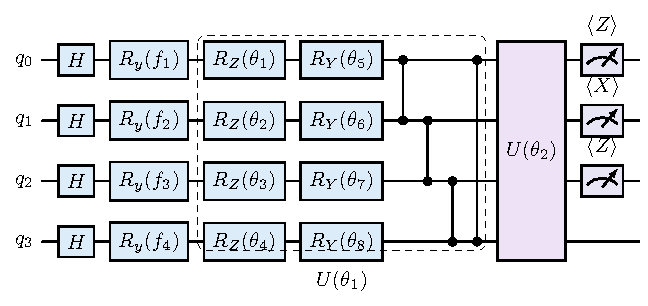
\includegraphics[width=0.90\textwidth]{figures/classifier_expectation.pdf}
  \caption{Binary expectation classifier: local measurements
  $\langle Z_0\rangle$, $\langle X_1\rangle$, and $\langle Z_2\rangle$ are
  averaged into the signed score in \cref{eq:classifier-binary-score}.}
  \label{fig:classifier-expectation-circuit}
\end{subfigure}

\vspace{5mm}
\begin{subfigure}{0.98\textwidth}
  \centering
  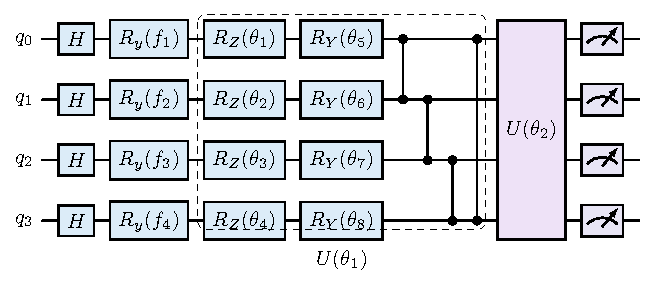
\includegraphics[width=0.90\textwidth]{figures/classifier_born_parity.pdf}
  \caption{Three-class Born classifier: the 16 probabilities of the four-wire
  basis distribution are aggregated by the external recursive-parity decoder in
  \cref{eq:classifier-parity-decoder}.}
  \label{fig:classifier-born-circuit}
\end{subfigure}
\caption{Classifier circuits traced from executable \code{PQCClassifier}
objects through \code{draw\_classifier(output="tikz")}.  The companion
\code{render\_classifier\_circuits.py} script retains standalone Quantikz,
vector PDF, and PNG outputs.  The decoder and sigmoid/softmax calibration are
classical post-processing and are therefore stated in the captions rather than
drawn as quantum gates.}
\label{fig:classifier-circuit-gallery}
\end{figure*}

\subsection{Objectives, training, and evaluation}
\label{sec:classifier-training}

The loss layer accepts class indices or, where applicable, one-hot targets.
For binary expectation scores, QASP encodes
$\widetilde y=2y-1\in\{-1,+1\}$ and provides
\begin{align}
  \mathcal L_{\mathrm{MSE}}
  &=\frac{1}{N}\sum_{i=1}^{N}(s_i-\widetilde y_i)^2,
  &
  \mathcal L_{\mathrm{hinge}}
  &=\frac{1}{N}\sum_{i=1}^{N}\max(0,1-\widetilde y_i s_i).
  \label{eq:classifier-score-losses}
\end{align}
For normalized class probabilities it provides binary and categorical cross
entropy,
\begin{align}
  \mathcal L_{\mathrm{BCE}}
  &=-\frac1N\sum_i\left[y_i\log p_i+(1-y_i)\log(1-p_i)\right],
  &
  \mathcal L_{\mathrm{CCE}}
  &=-\frac1N\sum_i\log p_{i,y_i}.
  \label{eq:classifier-probability-losses}
\end{align}
Multiclass MSE uses one-hot targets, and multiclass hinge uses the
Crammer--Singer margin between the target score and the largest competing
score.  Every objective supports \code{none}, \code{mean}, or \code{sum}
reduction.

\begin{qaspfeature}{\code{ClassifierLoss} and \code{ClassifierTrainer}}
\code{ClassifierLoss} dispatches MSE, hinge, binary cross entropy, or
categorical cross entropy without detaching the quantum computation graph.
\code{ClassifierTrainer} supplies a compact minibatch PyTorch loop with Adam
by default, user-provided optimizer support, validation histories, and held-out
evaluation.  The classifier chooses a compatible default objective, while an
explicit objective remains part of the experiment record.  Training targets
are integer class labels; observable groups in expectation readout are
arithmetic means, not the unit-weighted sums used by PQDQN per-action groups.
\end{qaspfeature}

\begin{qaspfeature}{Classification metrics}
\code{classification\_metrics} returns accuracy, balanced accuracy,
macro/per-class precision, recall, F1, support, and a confusion matrix.  When
probabilities are supplied it adds binary or one-vs-rest multiclass ROC AUC and
step-wise average-precision PR AUC.  Standalone helpers also provide top-$k$
accuracy, log loss, Brier score, and configurable macro, weighted, micro, or
per-class reductions.
\end{qaspfeature}

Confusion matrices place true labels in rows and predictions in columns.
Macro averages retain configured classes that are absent from the sample with
zero recall; multiclass Brier score sums squared class errors before averaging
examples.  ROC/PR AUC is undefined, and returned as NaN, when a binary sample
does not contain both classes.  These summaries are descriptive metrics, not
independent statistical significance tests.

The executed notebook
\code{examples/quantum\_classifiers\_sklearn\_validation.ipynb} exercises the
full public path on four familiar datasets.  Its purpose is integration
validation rather than a performance comparison: samples and epoch counts are
deliberately small, and no accuracy threshold is asserted.

\begin{table}[H]
\centering
\caption{Executable classifier integration coverage.  Every case checks output
shape, probability normalization, finite quantum gradients, training and
evaluation, and exact agreement of QASP accuracy, macro-F1, and confusion
matrices with scikit-learn.}
\label{tab:classifier-validation}
\small
\begin{tabularx}{\textwidth}{@{}p{0.23\textwidth}p{0.11\textwidth}p{0.18\textwidth}p{0.17\textwidth}X@{}}
\toprule
Dataset & Classes & Readout & Decoder & Objective \\
\midrule
Breast Cancer Wisconsin & 2 & expectation & -- & mean squared error \\
Iris & 3 & probabilities & parity & categorical cross entropy \\
Wine & 3 & probabilities & contiguous & categorical cross entropy \\
Digits $0$--$3$ & 4 & probabilities & majority & categorical cross entropy \\
\bottomrule
\end{tabularx}
\end{table}

The notebook also checks decoder conservation, all four objective gradients,
class-prior diagnostics, standalone symbolic Quantikz generation, and ROC/PR
AUC against scikit-learn on deliberately imbalanced binary data with tied
scores.  The dedicated classifier test module contains 18 passing tests over
these contracts.  These checks establish internal consistency and
interoperability, not quantum advantage or dataset-level superiority.

\section{Generative learning}
\label{sec:generative}

The generative module reuses QASP's circuit dictionaries, device selection,
autodifferentiation, Pauli propagation, and drawing stack to learn distributions
of binary strings.  Its primary public entries are \code{PQCBM},
\code{create\_qcbm}, \code{draw\_qcbm}, and \code{PauliMMD}.

\subsection{Quantum-circuit Born-machine abstraction}

A quantum-circuit Born machine (QCBM) prepares
$|\psi_{\bm\theta}\rangle=U(\bm\theta)|0^{\otimes n}\rangle$ and represents
\begin{equation}
  q_{\bm{\theta}}(x)
  =\left|\langle x|\psi_{\bm\theta}\rangle\right|^2,
  \qquad x\in\{0,1\}^{n}.
  \label{eq:pqcbm-born}
\end{equation}
\code{PQCBM} accepts an ansatz/feature-map configuration, an existing
\code{CircuitBuilder}, or a probability-valued PennyLane QNode.  Angle and IQP
ansatzes use the same component dictionaries as the RL and classifier
factories.  A custom QNode retains its device, shots, differentiation method,
and measured-wire order; QASP does not silently reconfigure it.

The optional feature map has a deliberately narrow conditioning contract.  It
encodes one fixed vector shared by all target rows, rather than treating each
generated bit string as an input.  \code{AngleEmbedding},
\code{NeuralEmbedding}, custom feature-map classes, re-uploading, and
trainable input scales are supported.  Conditional data with a different input
for every row requires an external training loop.

\begin{qaspfeature}{\code{PQCBM}, \code{create\_qcbm}, and \code{draw\_qcbm}}
\code{PQCBM} is a configuration-driven Born-machine model and trainer with
Torch or PennyLane Autograd parameters, NLL or Gaussian MMD$^2$ objectives,
optional fixed-vector conditioning, minibatching, direct device sampling,
entropy diagnostics, and small-system natural gradients.  The factory copies
caller configurations and builders.  Drawing returns text, Matplotlib, or
editable Quantikz from the constructed circuit.  \code{BornMachine} remains a
deprecated Autograd/integer-sample compatibility subclass.
\end{qaspfeature}

\Cref{lst:genlearn} constructs the executed example through the high-level
factory.  Binary training data have shape $(N,n)$, and wire zero is the most
significant output bit.

\begin{lstlisting}[caption={Constructing, training, sampling, and drawing a
three-qubit QASP Born machine.},label={lst:genlearn}]
import numpy as np
from qasp import create_qcbm, draw_qcbm

data = np.array([[0, 0, 0], [1, 1, 1]] * 128)
config = {
    "ansatz": "AngleAnsatz",
    "ansatz_config": {
        "n_layers": 2, "rotations": "YZ",
        "include_imprimitive": True,
        "imprimitive": "CNOT",
        "imprimitive_pattern": "chain",
    },
    "loss": "mmd",
    "mmd_config": {
        "bandwidths": [0.5, 1.0, 2.0],
        "mode": "exact",
    },
    "device": "default.qubit",
    "seed": 7, "lr": 0.05,
}
model = create_qcbm(config, n_qubits=3, data=data)
params, history = model.train(steps=120)
bits = model.sample(2000)         # shape (2000, 3)
probs = model.get_probs()         # guarded small-system diagnostic
tex = draw_qcbm(
    model, output="tikz",
    tikz_options={"standalone": True, "compress": True},
)
\end{lstlisting}

\subsection{Probability and expectation objectives}
\label{sec:genlearn-mmd}

For probability-capable execution, QASP minimizes minibatch negative log
likelihood
\begin{equation}
  \mathcal{L}_{\mathrm{NLL}}
  =-\frac{1}{|\mathcal{B}|}\sum_{x\in\mathcal{B}}
    \log\!\left(q_{\bm{\theta}}(x)+\varepsilon\right).
  \label{eq:pqcbm-nll}
\end{equation}
The accompanying KL helper expects a complete target distribution rather than
binary observations.  NLL, complete-probability diagnostics, and model entropy
retain a $2^n$ output cost and are guarded by
\code{max\_probability\_qubits}.

The scalable-output alternative represents Gaussian-kernel MMD$^2$ as a
mixture of Pauli expectations.  For binary strings, squared Euclidean distance
is Hamming distance.  QASP takes each bandwidth $\sigma$ to be a standard
deviation,
\begin{equation}
  k_\sigma(x,y)
  =\exp\!\left[-\frac{\|x-y\|_2^2}{2\sigma^2}\right].
  \label{eq:pqcbm-gaussian}
\end{equation}
For a mask $a\in\{0,1\}^n$, define
$Z_a=\prod_{j:a_j=1}Z_j$ and
$\mu_p(a)=\E_{x\sim p}[(-1)^{a\cdot x}]$.  Drawing every mask bit
independently with probability
\begin{equation}
  r_\sigma=\frac{1-\exp[-1/(2\sigma^2)]}{2}
  \label{eq:pqcbm-mask-rate}
\end{equation}
gives
\begin{equation}
  \operatorname{MMD}^2(p,q_{\bm\theta})
  =\E_{a\sim\operatorname{Bernoulli}(r_\sigma)^{\otimes n}}
  \left[
    \left(\mu_p(a)-\langle\psi_{\bm\theta}|Z_a|
    \psi_{\bm\theta}\rangle\right)^2
  \right].
  \label{eq:pqcbm-pauli-mmd}
\end{equation}
This is the expectation-mixture identity of
Recio-Armengol, Ahmed, and Bowles \cite{recioarmengol2025train}.  Their supplied
v1 uses $\sigma^2$ in its Gaussian-kernel definition but prints $\sigma$ in a
later mask formula.  QASP consistently follows the standard-deviation
convention in \cref{eq:pqcbm-gaussian,eq:pqcbm-mask-rate}; regression tests
compare the full loss and gradient with the dense Gaussian kernel at nonunit
bandwidths.

\begin{qaspfeature}{\code{PauliMMD}}
\code{PauliMMD} supports equal-weight bandwidth mixtures, Monte Carlo masks or
exact small-system enumeration, empirical target moments or a data
U-statistic correction, and isolated mask seeds.  The identity mask retains
its original probability mass.  Sampled mode avoids enumerating the Born
vector; exact mode is guarded because it enumerates all $2^n$ masks.
\end{qaspfeature}

For \code{estimator=\"unbiased\"} and $N\geq2$, the empirical data-square term
is replaced by
\begin{equation}
  \widehat{\mu_p(a)^2}_{\,U}
  =\frac{N\widehat{\mu}_p(a)^2-1}{N-1},
  \label{eq:pqcbm-data-u}
\end{equation}
which may be negative and is not clipped.  With finite circuit shots, QASP
evaluates the model moment twice independently and uses
$(\widehat\mu_{q,1}-\widehat\mu_p)
(\widehat\mu_{q,2}-\widehat\mu_p)$, avoiding the upward bias from squaring one
shot estimate.  Data minibatching, mask sampling, measurement shots, and
Pauli-propagation truncation remain distinct approximation sources.

\subsection{Training, execution, and sampling contracts}

\code{interface=\"torch\"} exposes live float64 tensors and Adam by default;
\code{interface=\"autograd\"} uses PennyLane NumPy and PennyLane optimizers.
Initialization can be uniform on $[0,2\pi)$, zero, or normally distributed,
and explicit parameter tensors are accepted.  \code{train} and its
\code{fit} alias return the final ansatz parameters and pre-update loss
history.  Torch users can replace \code{model.opt}, supply an optimizer factory,
or call differentiable \code{loss()} in an external loop.  A custom
\code{loss\_fn(probabilities,batch\_indices)} is a probability-readout path and
is therefore unavailable to the Pauli-propagation backend.  The tested
small-system natural-gradient option follows \cref{eq:naturalgradient}.

\begin{table}[H]
\centering
\caption{Principal PQCBM execution routes.  Availability of a particular
plugin, gate, measurement, or derivative combination remains the installed
PennyLane device's responsibility.}
\label{tab:pqcbm-backends}
\small
\begin{tabularx}{\textwidth}{@{}p{0.23\textwidth}p{0.19\textwidth}X@{}}
\toprule
Backend route & Objective/readout & Contract \\
\midrule
\code{default.qubit} & NLL probabilities or MMD moments & Analytic backprop, or finite-shot parameter shift where supported. \\
Lightning statevector/Kokkos/GPU & Probabilities with a supported method; analytic MMD moments with adjoint & MPI and plugin options pass through explicitly; no serial fallback. \\
\code{default.mixed} and other plugins & Device-supported probabilities or moments & Noise, shots, gates, and differentiation follow the plugin contract. \\
\code{lightning.pp} & Analytic Torch MMD moments & Differentiable Pauli propagation; no probabilities, finite shots, or MPI. \\
\bottomrule
\end{tabularx}
\end{table}

Pauli-propagation controls expose maximum retained Pauli weight, top-$M$
pruning, a coefficient threshold, and pruning cadence.  Unpruned, untruncated
propagation provides a feasible exact reference for small circuits, but exact
operator growth can still be exponential.  Truncated or pruned runs propagate
gradients only through retained paths and have no blanket efficiency or
unbiasedness guarantee.

\code{sample()} executes a sampling measurement directly; it does not first
construct a probability vector.  The default result is a
$(\text{shots},n)$ bit matrix, with optional big-endian indices up to 62 bits.
Because the PP engine produces expectations rather than samples, a PP-trained
model must name a separate sampling device:
\Needspace{15\baselineskip}
\begin{lstlisting}[caption={Training with Pauli propagation and deploying the
same learned circuit to a sampling backend.},label={lst:genlearn-pp}]
pp = create_qcbm(
    {**config, "device": "lightning.pp",
     "pp_prune": False},
    n_qubits=3, data=data,
)
pp.train(120)
bits = pp.sample(
    2000, device="default.qubit",
    device_kwargs={"seed": 19},
)
\end{lstlisting}

\subsection{Executed three-qubit example}
\label{sec:pqcbm-example}

The executed notebook trains matched state-vector and unpruned PP models on
256 rows split equally between $000$ and $111$.  Both models use two
$R_Y/R_Z$ layers with CNOT chains, seed 7, Adam learning rate $0.05$, 120
updates, and exact MMD with bandwidths $0.5$, $1$, and $2$.  Full probabilities
are used only for this small-system validation; 2,000 final samples are drawn
directly from \code{default.qubit} with seed 19.

\begin{figure}[p]
\centering
\begin{subfigure}{0.96\textwidth}
  \centering
  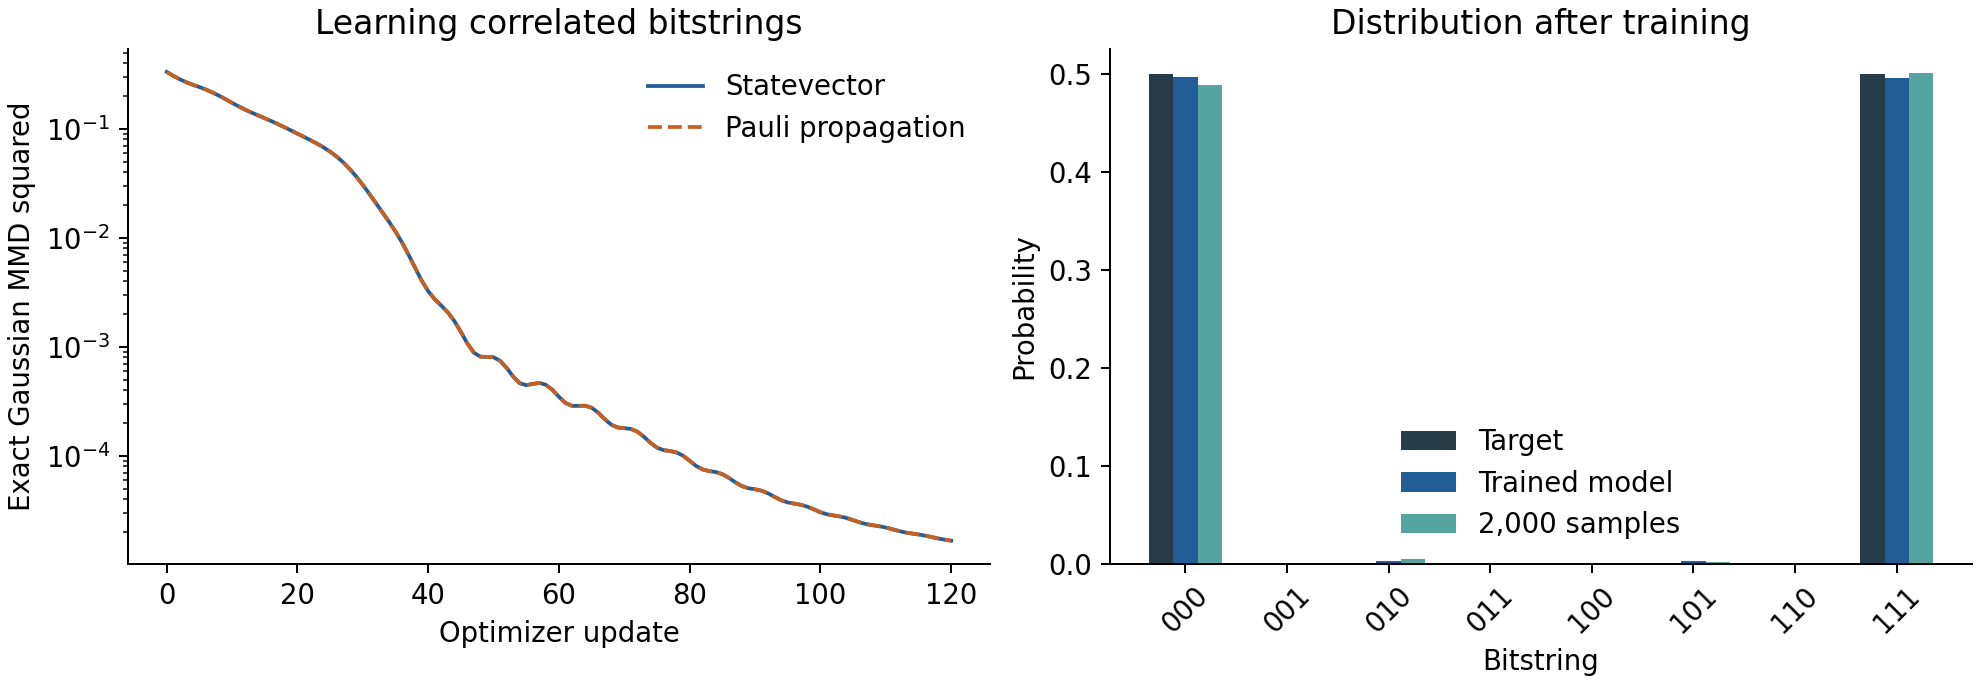
\includegraphics[width=\textwidth]{../examples/results/pqcbm_small_experiment/learning.png}
  \caption{State-vector and exact unpruned-PP learning curves, followed by the
  target, trained probabilities, and empirical frequencies from 2,000 direct
  device samples.}
\end{subfigure}

\vspace{4mm}
\begin{subfigure}{0.78\textwidth}
  \centering
  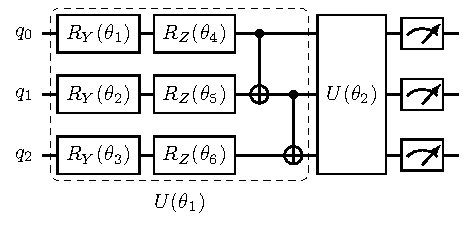
\includegraphics[width=\textwidth]{../examples/results/pqcbm_small_experiment/pqcbm.pdf}
  \caption{Paper-ready Quantikz exported from the trained \code{PQCBM}.  MMD is
  classical post-processing of measured Pauli moments and is not drawn as a
  quantum gate.}
\end{subfigure}
\caption{Reproducible PQCBM example generated by QASP.  The experiment is a
three-qubit, one-seed integration validation, not a scaling benchmark.}
\label{fig:pqcbm-example}
\end{figure}

\begin{table}[H]
\centering
\caption{Measured outcomes from the executed example in
\cref{fig:pqcbm-example}.  PP uses neither pruning nor weight truncation.}
\label{tab:pqcbm-example}
\small
\begin{tabularx}{0.82\textwidth}{@{}Xr@{}}
\toprule
Quantity & Value \\
\midrule
Initial MMD$^2$ & $0.3320805127$ \\
Final MMD$^2$ & $1.6678373\times10^{-5}$ \\
Probability on $\{000,111\}$ & $0.9925771886$ \\
Total variation from target & $0.0074228114$ \\
Initial gradient max difference, PP vs.\ statevector & $1.39\times10^{-16}$ \\
Final probability max difference, PP vs.\ statevector & $2.22\times10^{-16}$ \\
\bottomrule
\end{tabularx}
\end{table}

These values establish agreement for one tiny matched circuit, not a runtime or
scaling advantage.  QASP implements the reference paper's
expectation-mixture identity with its own execution engines; it does not
implement that work's specialized IQP Monte Carlo estimator, data-dependent
initialization, or thousand-qubit experiments.

\subsection{MPI and high-performance use}

For MPI-enabled statevectors, every rank must use the same parameters, data,
masks, optimizer state, seed, and circuit-call order.  MPI distributes one
simulator state rather than partitioning the data batch.  The HPC inspector
recognizes an MMD workload as an expectation output with a declared observable
batch instead of charging it for a $2^n$ probability vector.  Statevector
memory remains exponential, and exact-mask MMD retains exponential classical
storage.  The Deucalion helper supplies a rank-consistent callback and
collective smoke script, while the pure-statevector planner rejects PP,
noisy, and tensor methods because their memory models differ.

The local validation compares values, gradients, and updates across the
default state-vector simulator, Lightning state-vector and Kokkos devices, the
default mixed-state simulator, and unpruned QASP Pauli propagation.  It covers
Angle and IQP ansatzes; Torch and Autograd; finite-shot parameter shift; fixed
conditioning and input scales; Fisher updates; wire ordering; drawings; a
70-wire expectation-only PP smoke case; and local HPC routing.  It does not
constitute an actual multi-node MPI, GPU, tensor-network, or quantum-hardware
execution.

\section{Combinatorial optimization}
\label{sec:optimization}

The optimization module adds an end-to-end path from a classical binary
objective to a sampled assignment.  It separates the problem representation,
quantum algorithm, classical outer-loop optimizer, and final sampling budget,
while preserving a common result and circuit-drawing contract.  The supported
families are standard and multi-angle QAOA, relaxation-based warm-start QAOA,
recursive QAOA, fixed linear-ramp QAOA, and Pauli correlation encoding (PCE).
The implementations follow their respective algorithmic constructions
\cite{farhi2014qaoa,egger2021warm,bravyi2020rqaoa,herrman2022multiangle,
sciorilli2025pce,montanez2025lrqaoa}; QASP's contribution is to expose them
through the package's existing circuit notation, device selection, testing,
results, and Quantikz export.

\begin{figure}[H]
\centering
\resizebox{0.98\textwidth}{!}{%
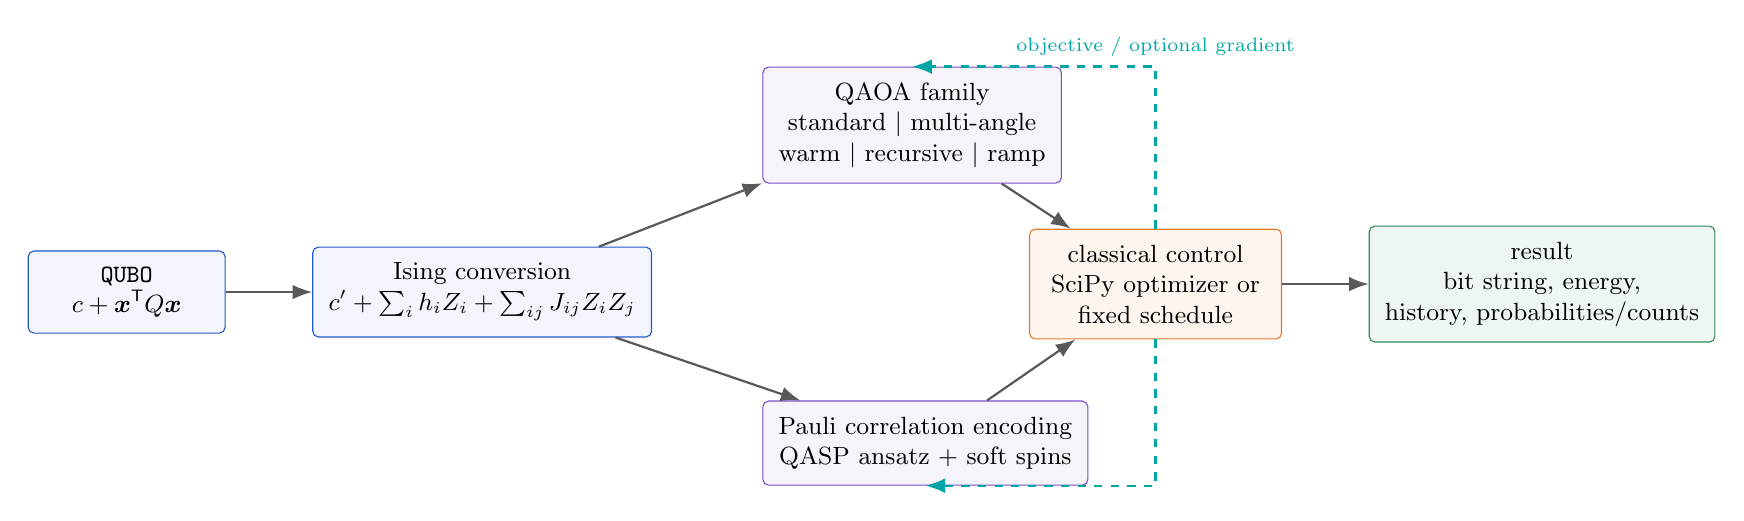
\begin{tikzpicture}[
  box/.style={draw,rounded corners=2pt,align=center,minimum height=10mm,inner sep=2mm,font=\small},
  problem/.style={box,draw=qaspblue,fill=qaspblue!6},
  quantum/.style={box,draw=qasppurple,fill=qasppurple!7},
  classical/.style={box,draw=qasporange,fill=qasporange!8},
  result/.style={box,draw=qaspgreen,fill=qaspgreen!8},
  flow/.style={-{Latex[length=2.5mm]},thick,draw=black!65},
  feedback/.style={-{Latex[length=2.5mm]},thick,dashed,draw=qaspcyan},
  node distance=8mm and 11mm
]
\node[problem,minimum width=25mm] (qubo) {\code{QUBO}\\$c+\bm x^{\mathsf T}Q\bm x$};
\node[problem,right=of qubo,minimum width=31mm] (ising) {Ising conversion\\$c'+\sum_i h_iZ_i+\sum_{ij}J_{ij}Z_iZ_j$};
\node[quantum,above right=8mm and 14mm of ising,minimum width=37mm] (qaoa) {QAOA family\\standard $\mid$ multi-angle\\warm $\mid$ recursive $\mid$ ramp};
\node[quantum,below right=8mm and 14mm of ising,minimum width=37mm] (pce) {Pauli correlation encoding\\QASP ansatz $+$ soft spins};
\node[classical,right=14mm of $(qaoa)!0.5!(pce)$,minimum width=32mm] (outer) {classical control\\SciPy optimizer or\\fixed schedule};
\node[result,right=of outer,minimum width=34mm] (output) {result\\bit string, energy,\\history, probabilities/counts};

\draw[flow] (qubo) -- (ising);
\draw[flow] (ising) -- (qaoa);
\draw[flow] (ising) -- (pce);
\draw[flow] (qaoa) -- (outer);
\draw[flow] (pce) -- (outer);
\draw[flow] (outer) -- (output);
\draw[feedback] (outer.north) |- node[above,font=\scriptsize,text=qaspcyan]{objective / optional gradient} (qaoa.north);
\draw[feedback] (outer.south) |- (pce.south);
\end{tikzpicture}}
\caption{Optimization dataflow in QASP.  A single QUBO representation supplies
an exact Ising Hamiltonian to multiple solver families.  Variational solvers
return objective values to a reusable classical optimizer, while LR-QAOA uses
a deterministic schedule.  Every route decodes to the original variable
ordering and records algorithm-specific metadata.}
\label{fig:optimization-stack}
\end{figure}

\subsection{QUBO and Ising problem contract}
\label{sec:qubo-contract}

For $n$ binary variables, QASP defines the quadratic unconstrained binary
optimization problem
\begin{equation}
  E_Q(\bm x)=c+\bm x^{\mathsf T}Q\bm x,
  \qquad \bm x\in\{0,1\}^{n}.
  \label{eq:qubo}
\end{equation}
Non-symmetric matrices are accepted: the two entries $Q_{ij}$ and $Q_{ji}$
are combined into one coefficient $b_{ij}=Q_{ij}+Q_{ji}$ for $i<j$.
Writing $a_i=Q_{ii}$ and substituting $x_i=(1-Z_i)/2$ produces
\begin{equation}
  H_C=c'I+\sum_i h_i Z_i+\sum_{i<j}J_{ij}Z_iZ_j,
  \label{eq:qubo-ising}
\end{equation}
where
\begin{equation}
  c'=c+\frac12\sum_i a_i+\frac14\sum_{i<j}b_{ij},\quad
  h_i=-\frac12a_i-\frac14\sum_{j\ne i}b_{\min(i,j),\max(i,j)},\quad
  J_{ij}=\frac14b_{ij}.
  \label{eq:qubo-ising-coefficients}
\end{equation}
Consequently $E_Q(\bm x)=\langle\bm x\rvert H_C\lvert\bm x\rangle$
under the computational-basis convention in \cref{eq:qubo-ising}.

\begin{qaspfeature}{\code{QUBO} and \code{PauliTerm}}
\code{QUBO} constructs objectives from a matrix, explicit linear/quadratic
terms, an Ising model, or a weighted MaxCut edge list.  It exposes exact
assignment energies, the offset and Ising coefficients, Pauli terms, a
PennyLane Hamiltonian including the constant, and a brute-force reference for
small instances.  \code{PauliTerm} is the shared weighted-Pauli representation
used by cost and mixer circuits.
\end{qaspfeature}

For weighted MaxCut, \code{QUBO.maxcut} returns the minimization objective
\begin{equation}
  E_{\mathrm{cut}}(\bm x)
  =-\sum_{(i,j)\in\mathcal E}w_{ij}
     \bigl(x_i+x_j-2x_ix_j\bigr),
  \label{eq:maxcut-qubo}
\end{equation}
so minimizing the returned energy maximizes the cut weight.  Keeping this sign
convention in the problem object prevents a solver-specific reinterpretation
of the reported energy.

\subsection{The QAOA family}
\label{sec:qaoa-family}

With cost Hamiltonian $H_C$ and mixer
$H_M=\sum_b m_bM_b$, depth-$p$ standard QAOA prepares
\begin{equation}
  \lvert\bm\gamma,\bm\beta\rangle
  =\prod_{\ell=1}^{p}
     e^{-i\beta_\ell H_M}e^{-i\gamma_\ell H_C}
     \lvert s\rangle,
  \qquad
  F(\bm\gamma,\bm\beta)
  =\langle\bm\gamma,\bm\beta\rvert H_C
     \lvert\bm\gamma,\bm\beta\rangle.
  \label{eq:qaoa-state}
\end{equation}
The constant term remains in $H_C$ for objective evaluation but does not
generate a circuit gate.  By default, $\lvert s\rangle=\lvert+\rangle^{\otimes n}$
and $H_M=\sum_iX_i$.  A QASP mixer dictionary can instead provide arbitrary
weighted Pauli words and a plus, zero, callable, or amplitude-vector initial
state.

Standard QAOA shares one cost angle and one mixer angle per layer.  In the
multi-angle variant, every nonconstant cost term $c_aP_a$ and mixer term
$m_bM_b$ receives its own parameter,
\begin{equation}
 U_C^{(\ell)}=\prod_a e^{-i\gamma_{\ell a}c_aP_a},
 \qquad
 U_M^{(\ell)}=\prod_b e^{-i\beta_{\ell b}m_bM_b},
 \label{eq:multiangle-qaoa}
\end{equation}
making standard QAOA the tied-parameter special case
\cite{herrman2022multiangle}.

\begin{qaspfeature}{\code{QAOA} and \code{WarmStartQAOA}}
\code{QAOA} supports standard or multi-angle parameters, QASP-style custom
mixers, random/zero/ramp initialization, Hamiltonian expectations, exact or
sampled probabilities, gradients, solution counts, and independent training
and reporting shot budgets.  \code{WarmStartQAOA} accepts a relaxed vector or
computes a bounded continuous QUBO relaxation before constructing the
warm-start initial state and mixer.
\end{qaspfeature}

For a relaxation $q_i\in[0,1]$, QASP clips the values to
$[\epsilon,1-\epsilon]$ and sets
\begin{equation}
  \vartheta_i=2\arcsin\sqrt{q_i},\qquad
  \lvert s_q\rangle=\bigotimes_iR_Y(\vartheta_i)\lvert0\rangle,
  \qquad
  H_M^{(q)}=-\sum_i\left(
    \sin\vartheta_iX_i+\cos\vartheta_iZ_i\right).
  \label{eq:warm-start-qaoa}
\end{equation}
This preserves the standard and multi-angle interfaces while changing both
the prepared state and, when no custom mixer is supplied, the mixer evolution
\cite{egger2021warm}.

\begin{qaspfeature}{\code{LRQAOA} / \code{LinearRampQAOA}}
Executes a deterministic opposing linear schedule without a classical
parameter optimizer.  With zero-based layer $\ell=0,\ldots,p-1$, QASP uses
$\gamma_\ell=(\ell+1)\Delta_\gamma/p$ and
$\beta_\ell=(1-\ell/p)\Delta_\beta$, with configurable increments and the
defaults $\Delta_\gamma=0.6$, $\Delta_\beta=0.3$.
\end{qaspfeature}

\begin{qaspfeature}{\code{RecursiveQAOA} / \code{RQAOA}}
At each reduction step, QASP optimizes a QAOA instance, evaluates the active
$\langle Z_i\rangle$ and $\langle Z_iZ_j\rangle$ correlations from its basis
probabilities, and rounds the largest-magnitude active Hamiltonian correlation.
A one-body rule fixes $Z_i=\pm1$; a two-body rule substitutes
$Z_j=\pm Z_i$.  Once the configured cutoff is reached, the reduced Ising
problem is solved exactly and all substitutions are reconstructed in reverse.
The result retains every elimination rule and intermediate QAOA result.
\end{qaspfeature}

\begin{lstlisting}[caption={Solving one MaxCut QUBO through the QASP QAOA family.},label={lst:optimization-qaoa}]
from qasp import (
    LRQAOA, QAOA, QUBO, RecursiveQAOA, WarmStartQAOA,
    draw_optimization,
)

problem = QUBO.maxcut(3, [(0, 1), (1, 2), (0, 2)])

# One parameter per cost and mixer gate; use analytic adjoint gradients.
multi = QAOA(
    problem, n_layers=2, parametrization="multi_angle", seed=7,
)
multi_result = multi.solve(
    optimizer="BFGS", use_gradients=True,
    optimizer_options={"maxiter": 30}, result_shots=2_000,
)

# A supplied vector or True enables relaxation-based warm starting.
warm_result = WarmStartQAOA(
    problem, n_layers=2, warm_start=True, seed=7,
).solve(optimizer_options={"maxiter": 30})

# Recursive reduction and a deterministic schedule use the same QUBO.
recursive_result = RecursiveQAOA(
    problem, cutoff=2, optimizer_options={"maxiter": 20},
).solve()
ramp_result = LRQAOA(problem, n_layers=4).solve()

paper_tikz = draw_optimization(
    multi, parameters=multi_result, output="tikz",
    tikz_options={"standalone": True,
                  "symbolic_parameters": True},
)
\end{lstlisting}

\subsection{Pauli correlation encoding}
\label{sec:pce}

PCE assigns each of $m$ optimization variables to an equal-Pauli
$k$-body correlation observable $P_i$ on an $n$-qubit variational state
\cite{sciorilli2025pce}.  For a chosen Pauli alphabet $\mathcal P$, the
available capacity is
\begin{equation}
  m_{\max}=|\mathcal P|\binom{n}{k};
  \qquad \mathcal P=\{X,Y,Z\},\ k=2
  \quad\Longrightarrow\quad
  m_{\max}=3\binom{n}{2}.
  \label{eq:pce-capacity}
\end{equation}
QASP selects the smallest $n$ meeting this capacity unless the register size
is supplied explicitly.  The measured correlations become smooth spins
\begin{equation}
  s_i(\bm\theta)=\tanh\!\left(
    \alpha\langle\psi_{\bm\theta}\rvert P_i
    \lvert\psi_{\bm\theta}\rangle\right),
  \label{eq:pce-soft-spin}
\end{equation}
and the implemented relaxed Ising objective is
\begin{equation}
  \mathcal L_{\mathrm{PCE}}(\bm\theta)
  =c'+\sum_i h_i s_i+\sum_{i<j}J_{ij}s_is_j
   +\lambda\nu\left(\frac1m\sum_i s_i^2\right)^2,
  \qquad
  \nu=\frac{|\mathcal E_Q|}{2}+\frac{m-1}{4},
  \label{eq:pce-loss}
\end{equation}
where $|\mathcal E_Q|$ is the number of nonzero quadratic Ising couplings.
Decoding uses $x_i=0$ for $s_i\ge0$ and $x_i=1$ otherwise, consistently with
$x_i=(1-Z_i)/2$.

\begin{qaspfeature}{\code{PauliCorrelationEncoding} / \code{PCE}}
Builds the correlation assignment, accepts \code{AngleAnsatz},
\code{IQPAnsatz}, an ansatz class/object, or a preconfigured
\code{CircuitBuilder}, measures all encoded correlations, optimizes the
soft-spin loss, and decodes to the original QUBO variable count.  The
\code{build\_pauli\_correlation\_encoding} helper exposes the register size and
ordered observable assignment before a solver is constructed.
\end{qaspfeature}

\begin{lstlisting}[caption={Qubit-compressed PCE with a dictionary-defined QASP ansatz.},label={lst:optimization-pce}]
from qasp import PCE, draw_pce

pce = PCE(problem, circuit={
    "ansatz": "AngleAnsatz",
    "ansatz_config": {
        "n_layers": 1,
        "rotations": ["Y 0", "Y 1", "ZZ 0 1"],
        "include_hadamards_initial": True,
    },
    "device": "default.qubit",
}, seed=7)

pce_result = pce.solve(optimizer_options={"maxiter": 30})
assert len(pce_result.bitstring) == problem.n_variables
pce_tikz = draw_pce(
    pce, parameters=pce_result, output="tikz",
    tikz_options={"standalone": True,
                  "symbolic_parameters": True},
)
\end{lstlisting}

\begin{figure*}[p]
\centering
\begin{subfigure}{0.98\textwidth}
  \centering
  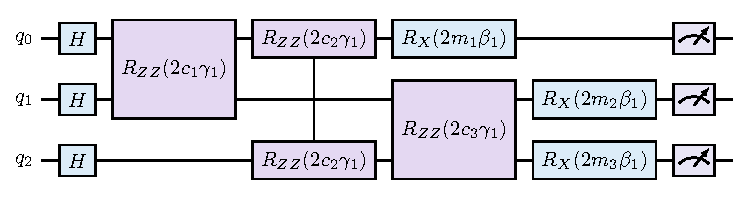
\includegraphics[width=0.86\textwidth]{figures/optimization_qaoa.pdf}
  \caption{One-layer standard QAOA for triangle MaxCut.  QASP derives the
  three $ZZ$ cost rotations from the QUBO, inserts the default $X$ mixer, and
  labels the shared parameters $\gamma_1$ and $\beta_1$.}
  \label{fig:optimization-qaoa-circuit}
\end{subfigure}

\vspace{6mm}
\begin{subfigure}{0.98\textwidth}
  \centering
  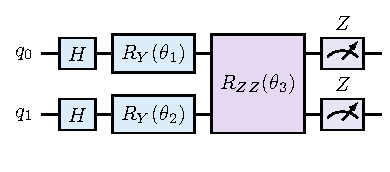
\includegraphics[width=0.68\textwidth]{figures/optimization_pce.pdf}
  \caption{Two-qubit PCE ansatz for the three-variable problem.  The terminal
  $Z$-basis trace depicts the $ZZ$ correlation setting; the same PCE object
  evaluates the corresponding $XX$ and $YY$ settings to encode all three
  variables.}
  \label{fig:optimization-pce-circuit}
\end{subfigure}
\caption{Optimization circuits generated from executable QASP objects by
\code{draw\_optimization}.  The companion renderer saves editable standalone
Quantikz, vector PDF, and PNG outputs; no circuit is redrawn manually.}
\label{fig:optimization-circuit-gallery}
\end{figure*}

\subsection{Classical control, results, and executable validation}
\label{sec:optimization-results}

\begin{qaspfeature}{Optimizers, results, and drawing}
\code{create\_optimizer} resolves COBYLA, Nelder--Mead, Powell, BFGS,
L-BFGS-B, SLSQP, or a user callable behind one SciPy-compatible interface.
\code{OptimizationResult} records parameters, decoded bit string, exact QUBO
energy, optimized quantum objective, optional probabilities or counts, shots,
history, status, metadata, and the raw optimizer result.
\code{RecursiveQAOAResult} adds elimination rules and intermediate results.
\code{draw\_optimization}, \code{draw\_qaoa}, \code{draw\_pce}, and
\code{draw\_recursive\_qaoa} emit text, Matplotlib, or symbolic Quantikz.
\end{qaspfeature}

The two scalar fields have different semantics: \code{objective} is the
optimized expectation or PCE surrogate, whereas \code{energy} evaluates the
decoded binary candidate in the original QUBO.  A successful classical
optimizer status certifies neither that candidate's global optimality nor a
better approximation ratio than a classical baseline.  Probabilities may be
absent for counts-only or decoded results.  Dense basis probabilities grow as
$2^n$; requesting counts avoids that output allocation but does not remove the
underlying simulator-state cost.

Analytic QAOA uses adjoint differentiation by default; finite-shot training
uses parameter shift when a gradient is requested, or a derivative-free
optimizer can minimize the noisy expectation directly.  The independent
\code{result\_shots} argument controls only the post-training distribution and
counts.  This distinction is recorded in result metadata and prevents an
analytic training run from being mislabeled as a shot-based solution estimate.
PCE currently uses a SciPy outer loop over NumPy-valued expectation calls and
should not be described as an end-to-end autodifferentiable solver.

The executable \code{tests/optimization\_algorithms.ipynb} covers every solver
family, custom mixers, both warm-start parameterizations, analytic and
finite-shot gradients, sampled solutions, and standalone symbolic drawings.
The focused unit module contains 14 passing tests summarized in
\cref{tab:optimization-validation}.

\begin{table}[H]
\centering
\caption{Focused validation of the optimization module.  These are software
contract checks on small problems, not approximation-ratio or scaling claims.}
\label{tab:optimization-validation}
\small
\begin{tabularx}{\textwidth}{@{}p{0.24\textwidth}p{0.31\textwidth}X@{}}
\toprule
Area & Configurations & Checked invariant \\
\midrule
QUBO representation & Matrix, terms, Ising, triangle MaxCut & Energy equality under QUBO--Ising conversion and exact small-instance optimum \\
QAOA circuits & Standard, custom mixer, multi-angle & Parameter shape, normalized probabilities, one parameter per declared gate \\
Differentiation & Analytic adjoint, BFGS, finite-shot parameter shift & Finite gradients and agreement with central finite differences \\
QAOA variants & Standard/multi-angle warm starts, LR-QAOA, RQAOA & Clipping and metadata, exact ramp schedule, reduction and reconstruction \\
Sampling/results & Training shots and independent result shots & Normalized estimates, count totals, bit-string probability, recorded contracts \\
PCE and drawings & Dictionary ansatz, $100$-variable capacity, all drawing outputs & Encoding size, decoded shape, finite objective, symbolic standalone Quantikz \\
\bottomrule
\end{tabularx}
\end{table}

\section{Trainability and structural diagnostics}
\label{sec:diagnostics}

\qasp{} includes diagnostics intended to run directly on the same constructed
models and configurations used for training.

\begin{qaspfeature}{\code{barren\_plateau\_diagnoser}}
The lazy top-level diagnostic accepts an already constructed classifier,
trainable kernel, or RL policy and reinitializes its quantum parameters from a
named QASP distribution.  For scalar costs $C_s$ measured at $N$ independent
initializations, it returns the running curve and final estimator
\begin{equation}
  \widehat{\operatorname{Var}}[C]
  = \frac{1}{N-1}\sum_{s=1}^{N}(C_s-\bar C)^2.
  \label{eq:model-cost-concentration}
\end{equation}
The same initialization draws also produce a componentwise variance for the
raw circuit expectations before decoder, softmax, or loss post-processing.
Observable circuits expose their measured expectations directly; for Born
readouts, local $Z$ expectations are reconstructed from the measured basis
distribution.  QASP reports both each component variance and the scalar
variance of their arithmetic mean; the latter retains cross-observable
covariance rather than averaging marginal variances.  Thus the diagnostic
separates concentration introduced by the quantum circuit from concentration
introduced by the task cost.
A fixed embedded state estimates variance over parameters conditional on that
input; omitting the state samples a fresh input on every initialization and
therefore estimates the joint state--parameter variance.  Default scalar
outputs are one selected class probability, action probability, or pairwise
kernel similarity.  Classifier objectives and arbitrary user-defined scalar
cost functions are also accepted.  Original parameters and module mode are
restored after the experiment.  A PQDQN is handled as a generic model and
therefore requires an explicit scalar \code{cost\_function(model, state)}, for
example one selected Q-value or a true TD loss.  By default only quantum-layer
parameters are reinitialized; \code{parameter\_scope="all"} also includes
trainable classical parameters.
For a system-size study, the user supplies a qubit list and a model factory.
The diagnostic constructs the same model family at every requested width,
performs the full initialization ensemble independently at each width, and
returns cost and scalar-expectation variance arrays aligned with the qubit
list.  A state factory can provide one controlled fixed input of the proper
dimension at each width.  Componentwise expectation variances remain keyed by
width because their dimension may grow with the number of measured qubits.
\end{qaspfeature}

The following example diagnoses the expectation-readout classifier constructed
in \cref{lst:classifiers}.  A fixed input isolates parameter-initialization
variance, while the two reported fields separate variation of the selected
class probability from variation of the circuit expectations that feed the
classical readout.
\begin{lstlisting}[caption={Cost-level and pre-decoder concentration from the model-agnostic barren-plateau diagnoser.},label={lst:barren-plateau-diagnoser}]
from qasp import barren_plateau_diagnoser

diagnosis = barren_plateau_diagnoser(
    expectation,
    n_samples=2000,
    initialization="random_-pi_pi",
    state=torch.as_tensor(X_test[0]),
    output_index=1,
    parameter_scope="quantum",
    seed=17,
    return_samples=True,
)
cost_variance = diagnosis["cost_variance"]
raw_expectation_variance = diagnosis["expectation_variance"]
running_curve = diagnosis["cost_variance_by_sample"]
\end{lstlisting}

The width-sweep mode makes the system-size dependence explicit.  The notebook
\path{examples/barren_plateau_diagnoser_validation.ipynb} constructs the
same one-layer classifier at every width, fixes the embedded state to zero, and
uses the global observable $Z^{\otimes n}$.  Thus the only changing experimental
variable is $n$.  The complete executable call is reproduced in
\cref{lst:barren-plateau-width-sweep}.

\begin{lstlisting}[caption={Executable cost-concentration sweep as a function of qubit count.  The notebook uses 128 independent parameter initializations at each width.},label={lst:barren-plateau-width-sweep}]
def classifier_factory(n):
    global_z = f'{"Z" * n} ' + " ".join(map(str, range(n)))
    return create_classifier({
        "ansatz": "AngleAnsatz",
        "ansatz_config": {
            "n_layers": 1, "rotations": "Y",
            "include_imprimitive": True, "imprimitive": "CZ",
            "imprimitive_pattern": "chain", "reuploading": False,
        },
        "feature_map": "AngleEmbedding",
        "feature_map_config": {
            "features": n, "rotations": "Y",
            "imprimitive_pattern": "chain",
        },
        "readout": "expectation", "observables": [global_z],
        "init": "zeros", "device": "default.qubit",
        "diff_method": "backprop",
    }, n_qubits=n, n_classes=2)

qubit_list = list(range(2, 11))
sweep = barren_plateau_diagnoser(
    model_factory=classifier_factory,
    qubit_list=qubit_list,
    n_samples=128,
    initialization="random_-pi_pi",
    state_factory=lambda n: torch.zeros(n),
    output_index=1,
    seed=19,
)

plt.semilogy(qubit_list, sweep["cost_variance"], "o-")
plt.semilogy(
    qubit_list, sweep["expectation_value_variance"], "s--"
)
\end{lstlisting}

\begin{figure}[H]
  \centering
  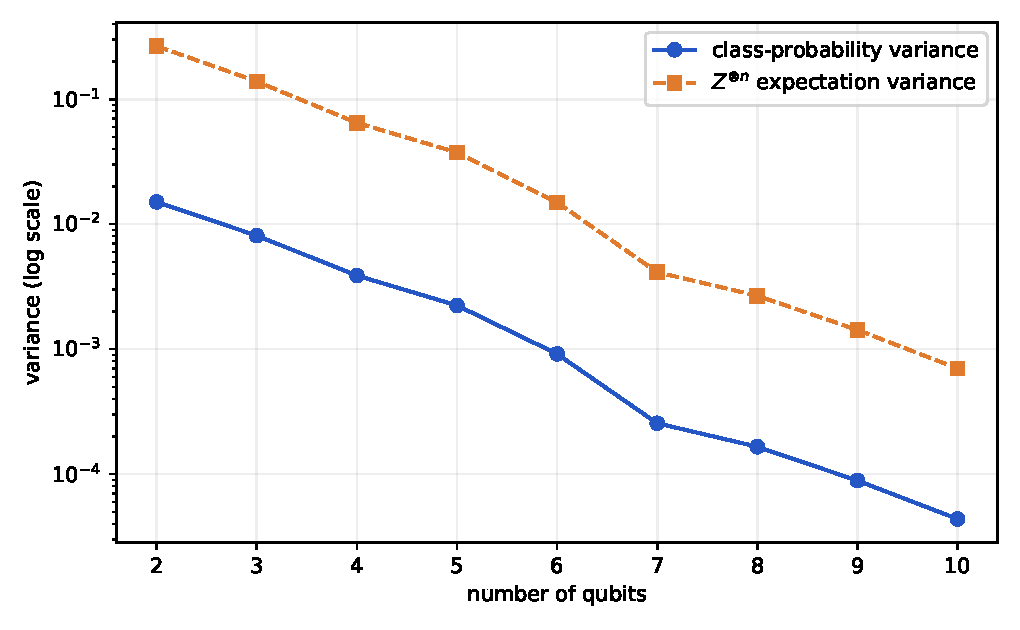
\includegraphics[width=0.74\textwidth]{figures/barren_plateau_variance_vs_qubits.pdf}
  \caption{Finite-size concentration experiment generated by the executable
  barren-plateau notebook.  Each point uses 128 independent
  $\operatorname{Unif}[-\pi,\pi]$ parameter initializations, a fixed zero input,
  a one-layer chain ansatz, and global $Z^{\otimes n}$ readout.  The raw
  expectation variance has fitted slope $-1.11$ per qubit on a base-two
  logarithmic scale over $n=2,\ldots,10$.  This cost-concentration example
  validates the width-sweep workflow; it is not, by itself, a claim about
  gradient-variance scaling.}
  \label{fig:barren-plateau-width-sweep}
\end{figure}

Cost concentration is a screening diagnostic rather than, by itself, a proof
of a barren plateau.  The conventional claim concerns exponential suppression
of gradient variance with system size \cite{mcclean2018barren}; a controlled
width sweep with a fixed cost, state protocol, and initialization distribution
is required for that conclusion.  The API records those choices explicitly so
cost-concentration experiments are not accidentally mixed across conditions.
The reported expectation statistic is variance across initialization draws,
not the single-state quantum measurement variance
$\langle O^2\rangle-\langle O\rangle^2$.

\begin{qaspfeature}{\code{policy\_variance}}
Repeatedly reinitializes a policy and estimates the variance of a selected
action probability across circuit sizes.  The controlled call, estimator, and
width sweep in
\cref{sec:cartpole-example,eq:policy-variance-estimator,lst:policy-variance}
make action and state conditioning explicit.  Samples can be distributed with
Ray, and qubit-dependent configuration values can be supplied as callables.
\end{qaspfeature}

For a compact single-policy sweep, the same public routine can be called as
follows; \code{raw\_samples[n]} retains the probabilities used to form each
width's variance estimate.  The more tightly controlled parity-versus-majority
experiment is given in \cref{lst:policy-variance}.
\begin{lstlisting}[caption={A width sweep of policy-output variance at fixed state and action.},label={lst:policy-variance-diagnostic}]
from qasp import policy_variance

variance, raw_samples = policy_variance(
    policy_class="PQCBorn",
    policy_config_kwargs=variance_policy_config,
    action=0,
    qubit_list=[3, 5, 7, 9],
    n_samples=500,
    batch_size=500,
    parallel=False,             # set True to distribute with Ray
    state=torch.zeros(4),       # omit for joint state/parameter variance
)
\end{lstlisting}

\begin{qaspfeature}{Legacy exploratory policy metrics}
\code{qasp.rl.metrics} retains policy-output sampling and heuristic structural
helpers used by earlier experiments.  The function named
\code{fourier\_analysis} currently performs no Fourier transform and also has
legacy import limitations.  \code{compute\_DLA\_generators} returns closure
sizes rather than generators, while \code{\_policy\_expressivity} and the
Hadamard/CZ/CNOT ``decomposition'' helpers assemble heuristic generator lists.
They are not certified circuit dynamical Lie algebras or executable unitary
gate decompositions.
\end{qaspfeature}

\cref{lst:dla-diagnostics} preserves the callable interface for reproducibility
while labelling the result correctly as an exploratory closure size.  Such a
quantity can motivate a follow-up symbolic analysis, but should not be used as
a proof of controllability or as a drop-in measure of policy expressivity.
\begin{lstlisting}[caption={Exploratory Lie-closure sizes and elements from the legacy policy-metrics interface.},label={lst:dla-diagnostics}]
from qasp import compute_DLA_generators, _policy_expressivity

dla_policy_config = {
    "ansatz": "AngleAnsatz",
    "ansatz_config": {
        "n_layers": 1, "rotations": "Y",
        "include_imprimitive": True, "imprimitive": "CZ",
        "imprimitive_pattern": "chain", "reuploading": False,
    },
    "feature_map": "AngleEmbedding",
    "feature_map_config": {
        "features": lambda n: n, "rotations": "Y",
    },
    "n_actions": 2, "policy": "contiguous-like",
    "training_method": "probs", "init": "normal_0_1",
    "device": "default.qubit", "diff_method": "backprop",
    "torchrl": False,
}

dla_dimensions = compute_DLA_generators(
    "PQCBorn", dla_policy_config, qubit_list=[2, 3, 4],
    parallel=False,
)
closure_3q = _policy_expressivity(
    "PQCBorn", dla_policy_config, n_qubits=3,
)
assert dla_dimensions[1] == len(closure_3q)
\end{lstlisting}

The validated diagnostics in this release are the finite-sample cost/output
concentration and policy-output variance estimators above.  The legacy
structural routines remain useful for hypothesis generation, but their names
must not be promoted into claims of Fourier spectra, certified Lie-algebra
dimensions, or task performance.

\section{Validation and reproducibility}
\label{sec:validation}

Release \version{} contains focused unit tests, executable notebooks,
cluster-oriented experiment drivers, and source-level API documentation for
all 52 Python modules and all 662 discovered definitions.  The documentation
pass added 385 missing definition docstrings and verified that removing
docstrings from before/after syntax trees leaves identical executable ASTs;
it did not modify runtime statements.  The policy/environment regression
suite checks not merely normalization,
but numerical equality of both forward action probabilities and backward
parameter gradients across exact representations.  The comparisons use
absolute and relative tolerance $10^{-6}$.  In the documented audit
environment, the existing suite produced 252 passes and one environment-only
failure out of 253 tests: the \code{lightning.kokkos} plugin was not installed
for one sparse-projector parametrization, while its
\code{lightning.qubit} counterpart passed.  That full-suite run used the
temporary Python 3.13 environment \code{/private/tmp/qasp-slurm-venv}.
After the intended Conda environment \code{torchlane} was identified, device
creation succeeded and only the previously failing Kokkos test was rerun: it
passed in 29.81 seconds without code changes under Python 3.10.17, PennyLane
0.42.2, Lightning/Lightning-Kokkos 0.42.0, Torch 2.7.0, and pytest 9.1.1.
This targeted result resolves the implementation concern but is not a claim
that all 253 tests were rerun together in \code{torchlane}.  Six small
package-guide examples also executed successfully.  These counts establish
coverage of the tested contracts, not validation of every legacy branch or
optional backend.

The completed generative-learning work was validated separately in
\code{torchlane}.  A broader regression selection produced 190 passes; after
the final API refinements, a focused selection produced 110 passes, including
43 generative cases plus existing MPI/HPC checks.  The selections overlap and
their counts are not additive.  Both emitted only the two expected
\code{BornMachine} deprecation warnings.  The checks cover dense-versus-Pauli
MMD values and gradients at nonunit bandwidths; Torch and Autograd; Angle and
IQP circuits; finite-shot parameter shift; fixed conditioning and trainable
scales; Fisher updates; wire order; direct sampling and drawings; and matched
\code{default.qubit}, Lightning, Kokkos, mixed-state, and unpruned-PP paths.
MPI routing used a serial stand-in, so this evidence does not replace an
actual collective cluster run.

\begin{table}[H]
\centering
\caption{Focused regression coverage for the revised RL policy layer.  The
full-probability backpropagation path is used as the reference where an
alternative exact representation is compared.}
\label{tab:rl-validation}
\small
\begin{tabularx}{\textwidth}{@{}p{0.23\textwidth}p{0.18\textwidth}X p{0.21\textwidth}@{}}
\toprule
Feature & Configurations & Checked invariant & Execution path \\
\midrule
Majority sparse projectors & $A=3$, six qubits & probabilities, normalization, and gradients & \code{lightning.qubit} adjoint in the full suite; targeted \code{lightning.kokkos} adjoint pass in \code{torchlane} \\
Multi-projector majority & $A=4$, six qubits & all parameter gradients agree after disabling device VJP & \code{lightning.qubit} adjoint \\
Ancilla-inclusive projector & $A=2$, five data qubits plus one ancilla & full-wire sparse operator and finite gradients & probability versus sparse-projector paths \\
Even majority block & $A=2$, six-wire block & all wires used; ties decode to zero; gradients agree & probability versus sparse-projector paths \\
Recursive parity moments & $A\in\{3,4\}$, six qubits & FWHT probabilities, normalization, and gradients & full probabilities versus logical expectations \\
PQDQN readouts & shared, per-action, parity, and majority & output shape, default/explicit bias, and finite gradients through circuit, input scales, and head & sequential and broadcast QNode paths \\
PQDQN Pauli backend & exact and truncated shared-$Z$ models & finite circuit/input-scale/head gradients, leading batch shape, target copying, drawing, and explicit device guards & QASP \code{lightning.pp}/backprop versus Lightning adjoint and \code{default.qubit} reference \\
Preset feature supports & parity/majority $a\in\{2,4\}$ & identity removal, term deduplication, independent features, and \code{preset\_actions} distinct from output actions & Walsh support extraction and explicit string checks \\
Historical compatibility & parity and majority projectors & explicit \code{preset\_mode="projectors"} reconstructs decoder probabilities with legacy shapes & expectation versus Born reference \\
Deep Q-learning & deterministic discrete environments & replay sampling, Double-DQN target, target synchronization, evaluation isolation, and termination masking & PyTorch trainer tests \\
Configuration guards & invalid derivative/device combinations & incompatible contracts raise explicit errors & constructor validation \\
Windy navigation & $A\in\{3,4\}$ & Gymnasium API, bounded observations, truncation, and seeded trajectory equality & environment-only tests \\
\bottomrule
\end{tabularx}
\end{table}

The repository's notebooks cover feature maps, model construction, policy
training, parameterized classifiers, QCBM/trainability experiments, IQP
variance analyses, and the complete combinatorial-optimization family.  The
package guide additionally provides six executed smoke examples and a complete
source inventory; the documentation audit records the 252-pass temporary-
environment suite, its missing-Kokkos-plugin failure, the subsequent targeted
Kokkos pass in \code{torchlane}, and executable-AST equivalence for the
docstring pass.  Neither notebook presence nor documentation coverage is
counted as validation of a legacy branch.
The
executed CartPole notebook additionally preserves 3,000 episodic returns
($2$ policies, $5$ seeds, and $300$ episodes), ten run times, and eight
fixed-state variance estimates as machine-readable CSV files.  The
executed PQDQN notebook adds 8,000 training episodes from 20 complete runs
(four readouts and five trained seeds), 2,800 greedy evaluation episodes,
per-run checkpoints and circuit metadata, and aggregate tables whose moving
statistics and held-out means were independently recomputed from the raw
records.  A separate executed ten-qubit PQDQN notebook preserves 420 raw timing
rows, 30 independently recomputed accuracy rows, matched states and inputs for
five parameter seeds, compact and expanded circuit exports, hardware and
dependency metadata, and source fingerprints.  Its fixed forward/gradient
workload adds no CartPole episodes and does not replace the four-qubit learning
study.  The companion observable-validation notebook checks finite gradients,
the $a=2$ and $a=4$ support lists, default and overridden bias semantics,
explicit historical projector compatibility, and a complete DQN smoke path.  The
policy-efficiency notebook adds matched CartPole and Windy Target Navigation
protocols, graph-IQP depth sweeps, automatic block diagnostics, parameter-copy
assertions, and explicit correction notes for superseded experimental runs.
The executed PQCBM notebook adds the complete three-qubit experiment from
\cref{sec:pqcbm-example}: 120 statevector and 120 matched unpruned-PP updates,
2,000 direct samples, saved loss/probability arrays, parameters, validation
metadata, and editable Quantikz output.
The \code{tests/tests\_deucalion} drivers provide contextual-bandit and CartPole
examples, parity actions, and scheduled cluster runs.  Because notebooks can
preserve outputs from different environments and development points,
publication-quality numerical claims must be regenerated from a tagged release
in a fresh environment rather than copied from exploratory cell output.

\subsection{Recommended experiment record}

For every reported result, we recommend recording:

\begin{enumerate}
  \item the QASP version, Git commit, Python version, and complete dependency lock file;
  \item random seeds for Python, NumPy, PyTorch, environment, and device where applicable;
  \item feature map, ansatz, topology, layer count, parameter initialization,
        ordered measured wires, decoder family, majority blocks and unused
        decoder wires, observables, action or class count, classifier readout,
        reference class prior, and calibration temperature;
  \item training method (probabilities, moments, or sparse projectors), device,
        shots, differentiation method, device-VJP and observable-batching
        settings, and hardware details;
  \item optimizer, objective, parameter groups, learning rates,
        batch/rollout size, baseline, entropy coefficient, gradient clipping,
        data split, preprocessing, and reported evaluation metrics;
  \item for value-based RL, the Pauli strings, feature matrix, preset mode,
        \code{preset\_actions}, environment \code{n\_actions}, explicit
        majority blocks, affine-bias choice, and resulting readout-parameter
        count; plus replay capacity, learning-start threshold,
        update and target-sync frequencies, Double-DQN choice, exploration
        schedule in frames, termination/truncation treatment, actual frame
        count, held-out reset seeds, and trained-seed unit of analysis;
  \item for combinatorial optimization, the exact QUBO matrix and offset,
        Ising convention, algorithm variant, depth, mixer and initial state,
        warm-start source and clipping, recursive cutoff and elimination
        rules, PCE correlation order/alphabet/register size, training and
        result shots, decoded energy, solution probability, and a feasible
        exact or classical reference;
  \item for Pauli propagation, $k$, $\tau$, top-$M$, pruning interval, peak retained terms, and error against a feasible exact reference;
  \item for Born-machine experiments, the ansatz, interface, initialization,
        target bit-matrix and any fixed conditioning vector; NLL versus MMD,
        bandwidth convention, mask mode/count/seed and estimator; minibatching,
        shots, independent finite-shot moment evaluation, PP truncation/pruning,
        natural-gradient Fisher and regularization choices, sampling backend,
        and probability-enumeration guards;
  \item for HPC execution, the hardware-profile date, inferred dimensions and
        explicit memory hints, analytical plan, Slurm script, actual allocation,
        MPI world layout, and measured peak memory/runtime as separate fields;
  \item wall-clock time separated into circuit construction, forward execution, gradient evaluation, and optimizer overhead.
\end{enumerate}

\subsection{Benchmark protocol for the release}
\label{sec:benchmark}

A defensible performance figure should compare equivalent observables and gradients, not merely backend API calls.  We propose the following release benchmark:

\begin{enumerate}
  \item Generate seeded ring and all-to-all \code{AngleAnsatz} circuits across $(n,L)$, with fixed local $Z$ and pairwise $ZZ$ observables.
  \item Measure forward and forward-plus-backward latency after one untimed warm-up for \code{default.qubit}, \code{lightning.qubit}, \code{lightning.kokkos}, \code{default.tensor}, and multiple Pauli truncation budgets.
  \item For approximate runs, report maximum and mean absolute expectation error and relative gradient error against the largest feasible exact state-vector instance.
  \item Publish medians and interquartile ranges over at least 20 parameter draws, together with peak resident memory and retained Pauli-term counts.
  \item Separate single-thread CPU, multi-thread CPU, GPU, and MPI results; never combine them in one scaling curve without explicit labels.
\end{enumerate}

The ten-qubit microbenchmark in \cref{sec:pqdqn-pp-benchmark} supplies one
machine-described point under this discipline.  It is not the proposed scaling
suite: broader circuit families, memory and retained-term measurements, more
parameter draws, and independently repeated machine sessions remain future
work.  Keeping that distinction explicit prevents a local microbenchmark from
becoming a release-wide performance guarantee.

The RL release benchmark should additionally preserve the following order of
evidence:
\begin{enumerate}
  \item verify probability and gradient equivalence of every specialized
        readout against the full-probability reference on small circuits;
  \item construct parity and majority policy pairs from the same graph-IQP
        configuration, copy the complete initial state dictionary, and assert
        elementwise equality before training;
  \item run the five-qubit proxy and ten-qubit cubic graph for
        $A\in\{3,4\}$, depths $L\in\{1,2,3\}$, and a published seed list;
  \item use identical environment and action-sampling seeds within every pair,
        and report random-policy and feedback-controller baselines;
  \item publish per-seed returns, waypoint success rates, time to a declared
        criterion, wall-clock time, and aggregate uncertainty rather than only
        a smoothed mean curve.
\end{enumerate}
This sequence distinguishes an implementation-equivalence claim from a policy
optimization result and, in turn, from a simulator-performance claim.

\section{Limitations and responsible interpretation}
\label{sec:limitations}

\qasp{} is research software at an alpha-stage release.  The following boundaries are material.

\begin{itemize}
  \item The package does not establish a quantum speedup, sample-complexity
        advantage, superior classification accuracy, or superior RL return.
        Those are properties of a fully specified algorithm, data-access
        model, baseline comparison, and execution regime.
  \item Generic state-vector simulation is exponential in qubit count.  Kokkos, batching, and MPI improve execution capacity but do not remove worst-case exponential memory.
  \item HPC placement and memory numbers are analytical estimates from a
        dated machine profile, not measured peak-memory or runtime guarantees.
        Rendering a Slurm script neither submits it nor verifies that the
        requested PennyLane plugin and MPI stack are installed.
  \item Pauli propagation is efficient only when the active operator expansion remains controlled.  Truncation introduces circuit- and parameter-dependent error; detached pruning masks yield piecewise gradients through retained terms.
  \item The current Pauli engines support CNOT, CZ, Hadamard, $R_X$, $R_Y$, $R_Z$, and one- or two-qubit \code{PauliRot} with $XX$, $YY$, or $ZZ$ generators, and require Pauli expectation measurements.
  \item Full-probability Born readout scales as $2^m$ in measured qubits.  Full
        moment reconstruction requires $2^m-1$ nontrivial $Z$ moments, although
        recursive parity reduces this to $2^{\lceil\log_2A\rceil}-1$ logical
        moments.
  \item Measuring only $A-1$ sparse majority projectors reduces the number of
        returned observables, not the Hilbert-space dimension: the current CSR
        construction still has dimension $2^{n+n_{\mathrm{anc}}}$ and is an
        exact small- and medium-system route rather than a polynomial-time
        simulator guarantee.
  \item Sparse-projector training depends on the standard Lightning adjoint
        path with device-native VJPs disabled.  This is a tested workaround for
        the current multi-projector stack and should be revalidated when the
        PennyLane-Lightning version changes.
  \item Automatic majority blocks are odd and nearly balanced, while explicit
        even blocks use tie-to-zero.  The decoder choice can therefore bias
        action or class masses before learning; block membership, unused wires,
        and the reference prior must be reported.
  \item Named \code{PQDQN} presets use an exponentially sized Walsh transform
        to discover Pauli support and are currently limited to 16 measured
        wires and $2^{22}$ projector-by-basis or feature-matrix entries.  The
        default exposes non-identity support terms independently; it does not
        reconstruct projector probabilities.  Pauli-expectation readouts can
        use QASP's \code{lightning.pp} selector with Torch backpropagation, but
        batches currently execute sample by sample and truncated gradients can
        differ substantially from an exact state-vector reference.  The
        ten-qubit microbenchmark shows that a faster small-$k$ workload need
        not preserve the quantum-gradient direction.  Without its classical
        head, bounded expectation features are generally a poor scale match
        for long-horizon action values.
  \item The completed CartPole Q-function comparison has five independently
        trained seeds per readout and no classical function-approximation
        baseline.  Feature counts, bias, and head-parameter counts differ; the
        majority model succeeds on several seeds and fails on one.  These
        variations and sub-475 held-out returns do not establish reliable
        solution, statistically demonstrated superiority, a general readout
        ranking, or quantum advantage.  A saved model state is also not an exact trainer
        resume unless optimizer, replay, and RNG states are preserved.
  \item A probability-readout classifier requires the complete $2^m$ Born
        vector on its measured wires in the current implementation.  An
        expectation classifier avoids that output dimension, but its
        sigmoid/softmax \code{predict\_proba} values are classical calibration
        of observable scores rather than directly measured Born probabilities.
  \item The bundled classifier notebook is an integration and gradient test on
        deliberately small preprocessed subsets.  It is not a competitive
        dataset benchmark, and the package does not presently implement
        cross-validation, early stopping, uncertainty calibration, or
        shot-aware confidence intervals in \code{ClassifierTrainer}.
  \item QAOA, warm-start QAOA, RQAOA, LR-QAOA, and PCE are heuristic solvers;
        the module does not guarantee an optimum or a better approximation
        ratio than a classical method.  \code{QUBO.brute\_force} is an
        exponential small-instance reference, not a scalable baseline.
  \item Exact QAOA probabilities require a $2^n$ output vector, while
        finite-shot objectives and correlations are noisy.  RQAOA inherits
        errors from every intermediate QAOA solve and finishes with an exact
        search exponential in the chosen cutoff.
  \item PCE compresses the number of qubits by assigning variables to Pauli
        correlations, but it does not by itself reduce the number of encoded
        observables or prove a runtime advantage.  The current PCE outer loop
        is NumPy/SciPy based rather than end-to-end autodifferentiable, and its
        regularized soft-spin relaxation is a heuristic surrogate.
  \item The automatic warm start is a locally solved box-constrained
        continuous QUBO relaxation, and the default LR-QAOA increments are a
        configurable schedule rather than a universal optimum.
  \item PQCBM NLL, complete-probability diagnostics, model entropy, exact-mask
        MMD, and dense Fisher matrices have exponential output, enumeration, or
        parameter-space costs and are small-system routes.  Sampled-mask MMD
        avoids enumerating outputs but does not make arbitrary circuits
        efficiently simulable.  Truncated/pruned PP has no general
        polynomial-time or unbiasedness guarantee, and PP-trained models need
        a separately selected device for sampling.  The supplied example has
        three qubits and one seed; it is an integration validation rather than
        a scaling result.  The Fisher kernel likewise enumerates basis scores,
        can be singular at zero probabilities, and currently ignores its
        legacy normalization option.
  \item \code{UQC}, \code{LearnablePQCBorn}, \code{qasp.rl.trl}, and legacy
        policy weight setters are retained historical paths with documented
        setup or post-processing restrictions.  Their presence does not imply
        validation in the current suite.
  \item \code{fourier\_analysis} performs no Fourier transform, and the legacy
        generator/decomposition helpers are exploratory lists or closure sizes,
        not certified dynamical Lie algebras or executable decompositions.
  \item Hardware support is inherited from installed PennyLane plugins, but device noise, queueing, calibration drift, and shot allocation are not abstracted away by \qasp{}.
  \item Some module-level RL utilities remain experimental and are not all re-exported from the top-level namespace.  Users should pin a release and import experimental classes from their defining module.
  \item \code{WindyTargetNavigationEnv} is a controlled software benchmark,
        not a substitute for a diverse RL task suite or evidence of practical
        control advantage.
\end{itemize}

These limitations motivate, rather than weaken, the package's explicit configuration model: a study can state exactly which approximation, decoder, and derivative estimator produced a result.

\section{Availability, extensibility, and research impact}
\label{sec:availability}

The source is available at \repo{} under the MIT license.  Installation from a release checkout uses \code{python -m pip install -e .}; development dependencies are available through the \code{dev} extra.  The declared runtime stack includes PennyLane, PyTorch, NumPy, SciPy, Gymnasium, TorchRL, TensorDict, Ray/RLlib, Matplotlib, and pandas.

The repository's package guide maps all 52 Python modules to their source
contracts and includes verified smoke examples for circuits and gradients,
Quantikz export, classifier training, fidelity kernels, QUBO evaluation, and
PQDQN output shapes.  The generative guide additionally records the complete
PQCBM construction, objective, backend, sampling, drawing, and cluster
contracts, together with the executed small-system validation.  Its
accompanying machine-readable documentation audit
records coverage, source hashes, the executable-AST equivalence check, and the
single optional-backend test limitation.  Documentation completeness should
not be read as evidence that every legacy branch or external plugin has been
validated.

New circuit components implement a small protocol: a feature map is callable
and declares its qubit/feature metadata; an ansatz is callable, references its
optional feature map, and reports parameter shapes.  New decoded-Born policies
extend the basis-state-to-action map in \code{\_PolicyDecoder}; classifier
partitions extend \code{ClassProbabilityDecoder}.  In both cases the existing
scatter-add and sample-lookup paths inherit the same declared semantics.
New Q-function readouts can provide explicit Pauli strings or derive a
non-identity Pauli support from a decoder preset.  The feature matrix $C$ is
the identity for shared and default preset features, while nested lists encode
fixed per-action sums.  \code{preset\_actions} controls only the preset
construction; the affine head still emits \code{n\_actions} environment
values.  \code{PQDQN} preserves the common circuit and autodifferentiation
boundary while \code{DeepQLearning} remains unaware of the chosen feature
construction or whether Pauli expectations came from a state vector or QASP's
differentiable Pauli engine.
New optimization algorithms can consume \code{QUBO.to\_ising} and return the
shared \code{OptimizationResult}; new QAOA mixers reuse the package's weighted
Pauli-word notation, while new compressed encodings can reuse
\code{CircuitBuilder} and the optimization drawing dispatch.
Specialized exact policy execution may add a corresponding moment or projector
construction, but it must be validated against
\code{training\_method="probs"}.  New execution strategies can consume the
builder's callable circuit or generated tape.  This separation makes it
possible to add a backend without rewriting task training, or add a decoder
without rewriting circuit construction.

The immediate research impact is methodological: \qasp{} consolidates
configurations and implementations that would otherwise be copied across
notebooks for QRL, quantum kernels, supervised classification, generative
learning, combinatorial optimization, and trainability studies.  Its reusable decoders and
exact-vs-approximate execution paths support controlled ablations of where
expressivity, gradient concentration, and simulation cost enter a quantum
learning model.  Concrete impact claims---external adopters, released
benchmark datasets, archived experiment artifacts, and papers enabled by the
package---should be added as they become citable: \todo{list publications,
external users, or archived datasets enabled by QASP, if available}.

\section{Conclusion}
\label{sec:conclusion}

\qasp{} organizes the full path from classical data to differentiable quantum
model and learning objective.  Its central abstraction is not a new circuit
language, but a reproducible connection between feature maps, ansatz
templates, label or action semantics, measurement representations, execution
backends, and gradient estimators.  The revised RL layer makes that separation
concrete: one vectorized decoder governs probability aggregation and sampled
actions; recursive parity has an exact logical-moment route;
majority--modulo has an exact sparse-projector route; and incompatible device
contracts fail explicitly.  The value-based path adds differentiable
Pauli-readout Q-functions, decoder-support feature presets, configurable affine
bias, and a replay-based Double-DQN trainer.  Its corrected five-seed CartPole
study demonstrates why the exact feature list, bias, head size, and
trained-seed variability must be reported: per-action sums have the highest
observed mean, shared features are more stable across these seeds, majority
learns on several seeds but fails on one, and parity does not learn useful
control under the stated budget.  These observations do not support a general
ranking.  The kernel layer adds unified
projector-configurable fidelity, projected expectation features, centered
alignment, and Fisher geometry.  The classifier layer then reuses the same
construction for Born-probability or expectation-score prediction, explicit
class decoders, supervised losses, training, and evaluation.  The generative
layer adds a configuration-driven PQCBM with probability NLL, exact or sampled
Pauli-expectation MMD, direct device sampling, optional conditioning, and
matched statevector/Pauli-propagation execution.  Its three-qubit example
demonstrates numerical equivalence at the reported settings without implying a
scaling advantage.  The optimization layer adds one QUBO/Ising contract for
standard, multi-angle, warm-start, recursive, linear-ramp, and
correlation-encoded solvers.  Together with accelerated conventional
simulation and differentiable Pauli propagation, these modules support
controlled comparisons across task families.  The ten-qubit PQDQN
microbenchmark illustrates the intended reporting standard: the observed
$k=2$ runtime reduction is presented together with its near-unit relative
quantum-gradient error, while the slower $k=3$ result rules out a blanket
backend ranking.  The public drawing path exports both interactive Matplotlib views
and publication-ready Quantikz source from the circuit objects that are
actually executed.  By making decoder semantics, projector locality, readout
contracts, and approximation budgets first-class configuration, \qasp{}
supports matched studies in which only the scientifically intended factor
changes.  The next priorities are a tagged benchmark suite with
accuracy--runtime and learning curves, broader unit coverage, stabilized
public exports, and archived release artifacts.

\section*{Author contributions}

Andr\'{e} Sequeira: conceptualization, software, methodology, investigation, and manuscript review.  \todo{revise the CRediT statement and add all software/paper contributors before submission}.

\section*{Acknowledgements}

\todo{add funding, institutional computing resources, and contributor acknowledgements; write ``None'' if not applicable}.

\section*{AI-use disclosure}

OpenAI Codex was used to assist with source-code inspection, literature discovery, diagram design, and preparation of an initial manuscript draft.  It was not treated as a source of experimental evidence.  All scientific claims, examples, references, and generated text must be checked by the named authors against the tagged software release before submission; responsibility for the final manuscript remains with the authors.

\section*{Data and software availability}

QASP source code, examples, the complete package guide, and the machine-readable
documentation audit are available at \repo{}.  The archival DOI for the exact
release described by this paper is \todo{create a Zenodo or equivalent archive for the release and insert its DOI}.  No new external dataset is required for the software description.  The corrected feature/bias PQDQN CartPole directory preserves its manifest, all raw training and evaluation records, seed-level summaries, checkpoints, and editable circuit figures; historical projector-reconstruction and aborted partial runs are kept separately and are not combined with it.  The separate ten-qubit simulator directory preserves raw timings, per-seed timing medians, accuracy rows, independently recomputed summaries, matched parameter/input checkpoints, hardware and verification metadata, source fingerprints, and editable circuit and plot exports.  The PQCBM example directory preserves its configuration, summary and
machine-readable validation, loss histories, target/model/sample
distributions, trained parameters, 2,000 sampled bit strings, and editable
Quantikz source.  These and the remaining reproducible benchmark outputs
should be attached to the archived release.

\bibliographystyle{unsrtnat}
\bibliography{references}

\clearpage
\appendix

\section{Configuration and API reference}
\label{app:api}

\begin{table}[H]
\centering
\caption{Principal public entry points and their role.  Experimental module-level classes are listed separately in the text.}
\scriptsize
\renewcommand{\arraystretch}{1.03}
\begin{tabularx}{\textwidth}{@{}p{0.28\textwidth}X@{}}
\toprule
Entry point & Purpose \\
\midrule
\code{CircuitBuilder} & Build a plain quantum function, bind its backend/QNode with \code{compile}, and allocate trainable weights through a Torch layer. \\
\code{AngleEmbedding}, \code{NeuralEmbedding} & Direct angle encoding and bias-free trainable linear-projection encoding; the neural reduction is currently single-sample. \\
\code{AngleAnsatz}, \code{IQPAnsatz} & Maintained general Pauli-rotation and commuting IQP-style circuit families; \code{UQC} is retained only as a historical function. \\
\code{create\_model}, \code{draw\_model} & Resolve model configurations and draw the executed circuit as Matplotlib output or editable Quantikz. \\
\code{circuit\_to\_tikz}, \code{save\_tikz} & Export a builder, tape, or callable circuit as styled Quantikz source, including symbolic parameters and repeated-layer compression. \\
\code{PQCBorn}, \code{PQCBornVariance} & Decoded-Born policies; the factory currently dispatches \code{"PQCBorn"} to the enhanced vectorized implementation with probability, moment, and sparse-projector paths. \\
\code{PQCSoftmax} & Pauli-expectation logits with an optional biased affine head; use \code{forward}, because the legacy \code{action\_probs} bypasses head, scaling, and PP execution. \\
\code{LearnablePQCBorn} & Historical adaptive-measurement prototype with known setup/post-processing limitations. \\
\code{PQDQN}, \code{create\_qfunction} & Differentiable action-value model and configuration factory with shared, per-action, parity, or majority Pauli features, configurable affine bias, preset size independent of output actions, and optional QASP \code{lightning.pp} execution. \\
\code{draw\_qfunction} & Draw the executable Q-function circuit as Matplotlib output or editable, compressed Quantikz. \\
\code{DeepQLearning} & Replay-based DQN/Double-DQN training with injectable optimizers, configurable replay/update/target/exploration schedules, observation transforms, gradient safeguards, and isolated greedy evaluation. \\
\code{REINFORCE}, \code{Reinforce} & Distinct episode-based policy-gradient implementations with different normalization, baselines, parameter groups, and stopping contracts. \\
\code{PPO}, \code{TorchRLTrainer} & Maintained clipped-PPO/GAE utility and an optional-version-dependent TensorDict/TorchRL adapter; \code{qasp.rl.trl} is legacy. \\
\code{BanditAWRConfig}, \code{ContextualBanditTrainer} & Advantage-weighted one-step training. \\
\code{WindyTargetNavigationEnv} & Seeded six-feature waypoint navigation with three or four discrete thrust actions. \\
\code{FastTruncatedPauliProp} & Non-differentiable packed-key expectation evaluator. \\
\code{FidelityKernel} & Unified global/localized overlap kernel configured by zero-state projector labels. \\
\code{ProjectedKernel} & Weighted Gaussian kernel over selected quantum expectation features. \\
\code{create\_kernel}, \code{draw\_kernel} & Resolve continuous-input kernel configurations and draw their evaluated circuits as Matplotlib or Quantikz. \\
\code{KernelTargetAlignment}, \code{align\_kernel} & Differentiate centered kernel--target alignment through trainable circuit parameters. \\
\code{QFKernel} & Small-system regularized Fisher-score Gram matrix with exhaustive basis enumeration and a currently unused normalization flag. \\
\code{PQCClassifier}, \code{QuantumClassifier} & Binary or multiclass parameterized classifiers with Born-probability or expectation-score readout. \\
\code{create\_classifier}, \code{draw\_classifier} & Resolve supervised model configurations and draw classifier circuits as text, Matplotlib, or Quantikz. \\
\code{ClassProbabilityDecoder} & Aggregate basis probabilities or decode samples with contiguous, parity, or majority class partitions. \\
\code{ClassifierLoss}, \code{ClassifierTrainer} & Differentiable supervised objectives and minibatch PyTorch training/evaluation. \\
\code{classification\_metrics} & Accuracy, confusion-matrix, precision/recall/F1, ROC-AUC, PR-AUC, log-loss, and Brier-score utilities. \\
\code{PQCBM}, \code{create\_qcbm} & Primary Born-machine model and configuration factory with Torch/Autograd, NLL or Pauli-expectation MMD, optional fixed conditioning, direct device sampling, and tested small-system natural gradients. \\
\code{PauliMMD} & Exact or sampled Gaussian-kernel mixtures over Pauli-$Z$ masks, bandwidth mixtures, empirical or data-U-statistic targets, and independent finite-shot model factors. \\
\code{draw\_qcbm} & Draw a configured or constructed Born machine as text, Matplotlib, or editable Quantikz; \code{BornMachine} is retained as a deprecated compatibility subclass. \\
\code{QUBO}, \code{PauliTerm} & Build binary objectives, convert exactly to Ising/Pauli form, evaluate assignments, and obtain small-instance references. \\
\code{QAOA}, \code{WarmStartQAOA} & Standard or multi-angle QAOA with custom mixers, gradients, analytic/finite-shot execution, and relaxation-based warm starts. \\
\code{RecursiveQAOA}, \code{RQAOA} & Correlation-driven variable elimination, exact cutoff solve, and reverse reconstruction. \\
\code{LRQAOA}, \code{LinearRampQAOA} & Fixed opposing linear schedules without classical parameter optimization. \\
\code{PauliCorrelationEncoding}, \code{PCE} & Correlation-compressed variables, QASP ansatz dictionaries, soft-spin optimization, and decoding. \\
\code{create\_optimizer}, \code{OptimizationResult} & Reusable SciPy optimizers and common solver outputs. \\
\code{draw\_optimization}, \code{draw\_qaoa}, \code{draw\_pce} & Draw optimization circuits as text, Matplotlib, or publication-ready Quantikz. \\
\code{policy\_variance} & Sampling-based variance of a selected policy output under controlled parameter/state initialization. \\
\code{fourier\_analysis} & Legacy helper that currently performs no Fourier transform; not a spectral-analysis claim. \\
\code{barren\_plateau\_diagnoser} & Cross-module cost-concentration variance with fixed or resampled embedded states. \\
\code{compute\_DLA\_generators} & Legacy exploratory Lie-closure sizes from heuristic generator lists, not returned generators or a certified circuit algebra. \\
\code{inspect\_workload}, \code{MemoryHints}, \code{plan\_deucalion} & Side-effect-free workload inspection and analytical memory/placement planning. \\
\code{create\_deucalion\_job}, \code{render\_slurm}, \code{ExecutionContext} & Generate (but do not submit) Slurm scripts and run MPI-aware callbacks with rank-consistent experiment seeds. \\
\bottomrule
\end{tabularx}
\end{table}

\section{Ancilla parity policy example}
\label{app:ancilla-parity}

For binary actions, recursive parity may be materialized as a circuit-level readout instead of computed from the full basis distribution.  Setting \code{parity\_cnot\_decomposition=True} makes the factory allocate one ancilla, append the required data-to-ancilla CNOT network, and measure the logical parity on that ancilla.  This changes the execution contract from a $2^m$ probability vector to an expectation-based readout while preserving the intended action semantics.

\begin{lstlisting}[caption={Building and drawing a binary ancilla-parity policy.  The generated circuit is \cref{fig:rl-ancilla-circuit}.},label={lst:ancilla-parity}]
from pathlib import Path
from qasp import create_model, draw_model
import torch

n_qubits = 4
ancilla_config = {
    "ansatz": "AngleAnsatz",
    "ansatz_config": {
        "n_layers": 1, "rotations": "ZY",
        "reuploading": False,
        "include_imprimitive": True, "imprimitive": "CZ",
        "imprimitive_pattern": "ring",
        "include_final_imprimitive": False,
        "include_feature_map_first": True,
        "include_hadamards_initial": True,
    },
    "feature_map": "AngleEmbedding",
    "feature_map_config": {
        "features": 4, "rotations": "Y", "input_scaling": False,
    },
    "n_actions": 2,
    "policy": "parity-like",
    "measurement_qubits": [0, 1, 2, 3],
    "training_method": "expectation",
    "parity_cnot_decomposition": True,
    "init": "small_normal",
    "device": "default.qubit",
    "diff_method": "backprop",
}
ancilla_policy = create_model("PQCBorn", ancilla_config,
                              n_qubits=n_qubits)
tikz = draw_model(
    model=ancilla_policy, inputs=torch.zeros(4), num_inputs=4,
    output="tikz",
    tikz_options={"standalone": True,
                  "symbolic_parameters": True,
                  "wire_labels": {4: "a_0"}},
)
Path("figures/rl_ancilla_parity.tex").write_text(tikz)
\end{lstlisting}

\section{Exact majority--modulo policy example}
\label{app:majority}

\begin{lstlisting}[caption={Drawing the probability-mode majority--modulo circuit and constructing its exact sparse-projector training variant.},label={lst:majority}]
from copy import deepcopy
from pathlib import Path
from qasp import create_model, draw_model
import torch

majority_config = {
    "ansatz": "AngleAnsatz",
    "ansatz_config": {
        "n_layers": 1, "rotations": "ZY", "reuploading": False,
        "include_imprimitive": True,
        "imprimitive": "CZ", "imprimitive_pattern": "ring",
        "include_final_imprimitive": False,
        "include_feature_map_first": True,
        "include_hadamards_initial": True,
    },
    "feature_map": "AngleEmbedding",
    "feature_map_config": {
        "features": 6, "rotations": "Y", "input_scaling": False,
    },
    "n_actions": 3,
    "policy": "majority-modulo",
    "measurement_qubits": [0, 1, 2, 3, 4, 5],
    "majority_blocks": [[0, 1, 2], [3, 4, 5]],
    "strict_majority_blocks": True,
    "training_method": "probs",
    "device": "default.qubit",
    "diff_method": "backprop",
    "shots": None,
    "init": "small_normal",
}
policy = create_model("PQCBorn", majority_config, n_qubits=6)

tikz = draw_model(
    model=policy, inputs=torch.zeros(6), num_inputs=6,
    output="tikz",
    tikz_options={"standalone": True,
                  "symbolic_parameters": True,
                  "compress": True},
)
Path("figures/rl_majority_modulo.tex").write_text(tikz)

# Same action semantics, but evaluate A - 1 exact projectors.
projector_config = deepcopy(majority_config)
projector_config.update({
    "training_method": "sparse_projectors",
    "device": "lightning.qubit",
    "diff_method": "adjoint",
})
training_policy = create_model("PQCBorn", projector_config, n_qubits=6)
\end{lstlisting}

The two majority bits encode four logical values; the final modulo operation maps them into three actions.  The sparse-projector path evaluates only $A-1=2$ projectors and reconstructs the last action probability as one minus their sum.  For this mode, \qasp{} includes identities on unmeasured wires and ancillas so each sparse operator spans the full device wire set.

\section{Exact multi-action recursive parity}
\label{app:multiaction-parity}

The expectation path below constructs the three nonidentity products of the
$k=2$ logical parity observables needed for four actions.  The circuit returns
those moments, the differentiable FWHT reconstructs the four logical-code
probabilities, and modulo aggregation is the identity because $A=2^k$.

\begin{lstlisting}[caption={Four-action recursive parity using exact logical moments rather than a $2^6$ probability vector.},label={lst:multiaction-parity}]
import torch
from qasp import create_model

parity4 = create_model("PQCBorn", {
    "ansatz": "IQPAnsatz",
    "ansatz_config": {
        "n_layers": 2,
        "imprimitive_pattern": "ring",
        "reuploading": True,
        "include_single_qubit": True,
    },
    "feature_map": "NeuralEmbedding",
    "feature_map_config": {"features": 6, "rotations": "Z"},
    "n_actions": 4,
    "policy": "parity-like",
    "measurement_qubits": list(range(6)),
    "training_method": "expectation",
    "parity_cnot_decomposition": False,
    "device": "lightning.qubit",
    "diff_method": "adjoint",
    "shots": None,
    "init": "normal_0_1",
}, n_qubits=6)

observation = torch.zeros(6)
probabilities = parity4(observation)
loss = -torch.log(probabilities[2])
loss.backward()
assert probabilities.shape == (4,)
assert any(
    parameter.grad is not None
    and torch.isfinite(parameter.grad).all()
    for parameter in parity4.parameters()
)
\end{lstlisting}

For $A=3$, the construction is identical except that the logical code $11_2$
is reduced modulo three and contributes to action zero.  This convention is
also used by direct sample decoding, so training and deployment remain
consistent for non-power-of-two action sets.

\section{Windy navigation with an exact majority policy}
\label{app:windy-example}

\Cref{lst:windy-policy} uses six observation features, two majority bits, and
three actions.  The full Hilbert-space probabilities are never returned by the
policy: two sparse action projectors are evaluated and the third probability
is the residual.  Passing the environment object directly to \code{REINFORCE}
uses the same Gymnasium interface as a registered environment name.

\begin{lstlisting}[caption={Three-action majority--modulo training on the bundled windy-navigation environment.},label={lst:windy-policy}]
from qasp import create_model, REINFORCE, WindyTargetNavigationEnv

n_qubits = 6
policy = create_model("PQCBorn", {
    "ansatz": "IQPAnsatz",
    "ansatz_config": {
        "n_layers": 2,
        "imprimitive_pattern": "ring",
        "reuploading": True,
        "include_single_qubit": True,
    },
    "feature_map": "NeuralEmbedding",
    "feature_map_config": {"features": 6, "rotations": "Z"},
    "n_actions": 3,
    "policy": "majority-modulo",
    "measurement_qubits": list(range(6)),
    "majority_blocks": [[0, 1, 2], [3, 4, 5]],
    "strict_majority_blocks": True,
    "training_method": "sparse_projectors",
    "device": "lightning.qubit",
    "diff_method": "adjoint",
    "shots": None,
    "init": "normal_0_1",
}, n_qubits=n_qubits)

environment = WindyTargetNavigationEnv(
    n_actions=3, max_episode_steps=180, n_waypoints=3
)
agent = REINFORCE(
    policy=policy,
    env_name=environment,
    logits=False,
    gamma=0.99,
    lr=2e-2,
    batch_episodes=5,
    normalize_mode="none",
    normalize_returns=True,
    entropy_coef=3e-2,
    baseline_type="ema",
    max_grad_norm=0.5,
    max_steps=180,
)
returns = agent.train(num_episodes=600)
\end{lstlisting}

\section{Release checklist}
\label{app:release}

The following items should be completed before the manuscript and repository are made public:

\begin{enumerate}
  \item replace author, affiliation, funding, impact, and archive placeholders;
  \item tag the exact commit as v\version{} and update \code{pyproject.toml} URLs to the public repository;
  \item stabilize public exports for module-level PPO and contextual-bandit APIs, and make the distinct \code{REINFORCE}/\code{Reinforce} names unambiguous;
  \item run the complete test suite in clean Python 3.10, 3.11, and 3.12 environments, install and exercise every advertised optional backend, and retain the current environment-specific failure record rather than hiding it;
  \item rerun the PQCBM backend matrix and executed notebook against the final
        release tag, retain the exact MMD/dense-kernel and PP/statevector
        equivalence records, and execute the supplied collective smoke test on
        the target MPI installation before making cluster claims;
  \item consolidate the TorchRL implementations, retire or repair \code{qasp.rl.trl}, and validate the maintained \code{TorchRLTrainer} against pinned TorchRL/TensorDict versions;
  \item repair or formally deprecate \code{UQC}, \code{LearnablePQCBorn}, legacy policy weight setters, and the misleading Fourier/DLA helper names;
  \item add exact-vs-approximate forward and gradient tests for both Pauli engines across all supported gates;
  \item publish the benchmark protocol from \cref{sec:benchmark} with machine-readable results;
  \item freeze an environment/lock file and archive the release with a DOI;
  \item render every example in the paper against the tag and record the command in continuous integration;
  \item run the optimization notebook and focused tests against the release tag,
        preserve small-instance exact energies, and benchmark every heuristic
        against declared classical references before making performance claims;
  \item select a venue and adapt the front matter and length: the present manuscript is a full preprint, while a Journal of Open Source Software submission would require a substantially shorter paper and venue-specific metadata.
\end{enumerate}

\end{document}
